\documentclass[twoside]{book}

% Packages required by doxygen
\usepackage{fixltx2e}
\usepackage{calc}
\usepackage{doxygen}
\usepackage[export]{adjustbox} % also loads graphicx
\usepackage{graphicx}
\usepackage[utf8]{inputenc}
\usepackage{makeidx}
\usepackage{multicol}
\usepackage{multirow}
\PassOptionsToPackage{warn}{textcomp}
\usepackage{textcomp}
\usepackage[nointegrals]{wasysym}
\usepackage[table]{xcolor}

% Font selection
\usepackage[T1]{fontenc}
\usepackage[scaled=.90]{helvet}
\usepackage{courier}
\usepackage{amssymb}
\usepackage{sectsty}
\renewcommand{\familydefault}{\sfdefault}
\allsectionsfont{%
  \fontseries{bc}\selectfont%
  \color{darkgray}%
}
\renewcommand{\DoxyLabelFont}{%
  \fontseries{bc}\selectfont%
  \color{darkgray}%
}
\newcommand{\+}{\discretionary{\mbox{\scriptsize$\hookleftarrow$}}{}{}}

% Page & text layout
\usepackage{geometry}
\geometry{%
  a4paper,%
  top=2.5cm,%
  bottom=2.5cm,%
  left=2.5cm,%
  right=2.5cm%
}
\tolerance=750
\hfuzz=15pt
\hbadness=750
\setlength{\emergencystretch}{15pt}
\setlength{\parindent}{0cm}
\setlength{\parskip}{3ex plus 2ex minus 2ex}
\makeatletter
\renewcommand{\paragraph}{%
  \@startsection{paragraph}{4}{0ex}{-1.0ex}{1.0ex}{%
    \normalfont\normalsize\bfseries\SS@parafont%
  }%
}
\renewcommand{\subparagraph}{%
  \@startsection{subparagraph}{5}{0ex}{-1.0ex}{1.0ex}{%
    \normalfont\normalsize\bfseries\SS@subparafont%
  }%
}
\makeatother

% Headers & footers
\usepackage{fancyhdr}
\pagestyle{fancyplain}
\fancyhead[LE]{\fancyplain{}{\bfseries\thepage}}
\fancyhead[CE]{\fancyplain{}{}}
\fancyhead[RE]{\fancyplain{}{\bfseries\leftmark}}
\fancyhead[LO]{\fancyplain{}{\bfseries\rightmark}}
\fancyhead[CO]{\fancyplain{}{}}
\fancyhead[RO]{\fancyplain{}{\bfseries\thepage}}
\fancyfoot[LE]{\fancyplain{}{}}
\fancyfoot[CE]{\fancyplain{}{}}
\fancyfoot[RE]{\fancyplain{}{\bfseries\scriptsize Generated by Doxygen }}
\fancyfoot[LO]{\fancyplain{}{\bfseries\scriptsize Generated by Doxygen }}
\fancyfoot[CO]{\fancyplain{}{}}
\fancyfoot[RO]{\fancyplain{}{}}
\renewcommand{\footrulewidth}{0.4pt}
\renewcommand{\chaptermark}[1]{%
  \markboth{#1}{}%
}
\renewcommand{\sectionmark}[1]{%
  \markright{\thesection\ #1}%
}

% Indices & bibliography
\usepackage{natbib}
\usepackage[titles]{tocloft}
\setcounter{tocdepth}{3}
\setcounter{secnumdepth}{5}
\makeindex

% Hyperlinks (required, but should be loaded last)
\usepackage{ifpdf}
\ifpdf
  \usepackage[pdftex,pagebackref=true]{hyperref}
\else
  \usepackage[ps2pdf,pagebackref=true]{hyperref}
\fi
\hypersetup{%
  colorlinks=true,%
  linkcolor=blue,%
  citecolor=blue,%
  unicode%
}

% Custom commands
\newcommand{\clearemptydoublepage}{%
  \newpage{\pagestyle{empty}\cleardoublepage}%
}

\usepackage{caption}
\captionsetup{labelsep=space,justification=centering,font={bf},singlelinecheck=off,skip=4pt,position=top}

%===== C O N T E N T S =====

\begin{document}

% Titlepage & ToC
\hypersetup{pageanchor=false,
             bookmarksnumbered=true,
             pdfencoding=unicode
            }
\pagenumbering{alph}
\begin{titlepage}
\vspace*{7cm}
\begin{center}%
{\Large Open\+CK \\[1ex]\large 0.\+0.\+1 }\\
\vspace*{1cm}
{\large Generated by Doxygen 1.8.13}\\
\end{center}
\end{titlepage}
\clearemptydoublepage
\pagenumbering{roman}
\tableofcontents
\clearemptydoublepage
\pagenumbering{arabic}
\hypersetup{pageanchor=true}

%--- Begin generated contents ---
\chapter{User Interface}
\label{md__c_1__users_alexa__documents__coding__qt_why_openck__open_c_k__u_i__r_e_a_d_m_e}
\Hypertarget{md__c_1__users_alexa__documents__coding__qt_why_openck__open_c_k__u_i__r_e_a_d_m_e}
This folder contains the vast majority of the User Interface code for CK, in addition to backend hooks.

The recommended way of editing/adding on to the UI is via Qt\textquotesingle{}s UI Designer via the .ui file. 
\chapter{Hierarchical Index}
\section{Class Hierarchy}
This inheritance list is sorted roughly, but not completely, alphabetically\+:\begin{DoxyCompactList}
\item \contentsline{section}{Form}{\pageref{class_form}}{}
\begin{DoxyCompactList}
\item \contentsline{section}{T\+E\+S4\+Form}{\pageref{class_t_e_s4_form}}{}
\end{DoxyCompactList}
\item \contentsline{section}{Form\+Header}{\pageref{struct_form_header}}{}
\item \contentsline{section}{Parser}{\pageref{class_parser}}{}
\item Q\+Dialog\begin{DoxyCompactList}
\item \contentsline{section}{Data\+Window}{\pageref{class_data_window}}{}
\end{DoxyCompactList}
\item Q\+Main\+Window\begin{DoxyCompactList}
\item \contentsline{section}{Main\+Window}{\pageref{class_main_window}}{}
\end{DoxyCompactList}
\item \contentsline{section}{Read\+File}{\pageref{class_read_file}}{}
\item \contentsline{section}{Subrecord\+Header}{\pageref{struct_subrecord_header}}{}
\end{DoxyCompactList}

\chapter{Class Index}
\section{Class List}
Here are the classes, structs, unions and interfaces with brief descriptions\+:\begin{DoxyCompactList}
\item\contentsline{section}{\hyperlink{class_data_window}{Data\+Window} \\*The data window class }{\pageref{class_data_window}}{}
\item\contentsline{section}{\hyperlink{class_form}{Form} \\*The base class for forms in .esp and .esm files }{\pageref{class_form}}{}
\item\contentsline{section}{\hyperlink{struct_form_header}{Form\+Header} \\*The header of the nonparsed form }{\pageref{struct_form_header}}{}
\item\contentsline{section}{\hyperlink{class_main_window}{Main\+Window} \\*In the UI }{\pageref{class_main_window}}{}
\item\contentsline{section}{\hyperlink{class_parser}{Parser} \\*The class that parses .esm/.esp files }{\pageref{class_parser}}{}
\item\contentsline{section}{\hyperlink{class_read_file}{Read\+File} }{\pageref{class_read_file}}{}
\item\contentsline{section}{\hyperlink{struct_subrecord_header}{Subrecord\+Header} \\*The parsed header for each subrecord }{\pageref{struct_subrecord_header}}{}
\item\contentsline{section}{\hyperlink{class_t_e_s4_form}{T\+E\+S4\+Form} \\*The class for the T\+E\+S4 header }{\pageref{class_t_e_s4_form}}{}
\end{DoxyCompactList}

\chapter{Class Documentation}
\hypertarget{class_data_window}{}\section{Data\+Window Class Reference}
\label{class_data_window}\index{Data\+Window@{Data\+Window}}


The data window class.  




{\ttfamily \#include $<$datawindow.\+h$>$}

Inheritance diagram for Data\+Window\+:\begin{figure}[H]
\begin{center}
\leavevmode
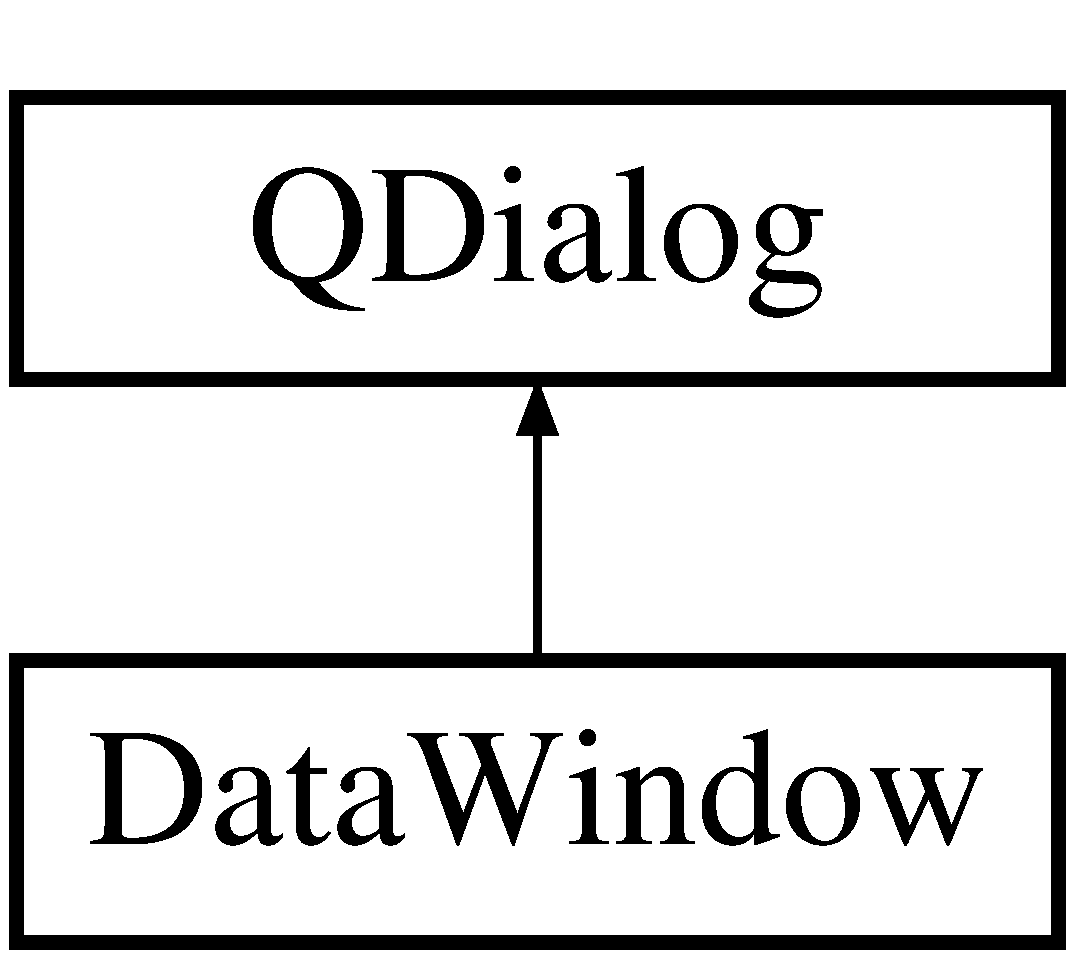
\includegraphics[height=2.000000cm]{class_data_window}
\end{center}
\end{figure}
\subsection*{Public Member Functions}
\begin{DoxyCompactItemize}
\item 
\hyperlink{class_data_window_aa4f27d2945b5cf6dd26e8b73bbc8aaa0}{Data\+Window} (Q\+Widget $\ast$parent=0)
\begin{DoxyCompactList}\small\item\em Constructs \& sets up the data window. \end{DoxyCompactList}\item 
\hyperlink{class_data_window_a6e72c3705abc085d3d84cb182493cd6a}{$\sim$\+Data\+Window} ()
\begin{DoxyCompactList}\small\item\em \hyperlink{class_data_window_a6e72c3705abc085d3d84cb182493cd6a}{Data\+Window\+::$\sim$\+Data\+Window}. \end{DoxyCompactList}\end{DoxyCompactItemize}
\subsection*{Private Slots}
\begin{DoxyCompactItemize}
\item 
void \hyperlink{class_data_window_a04f666600237b8807b990a274688fcca}{on\+\_\+button\+Box\+\_\+rejected} ()
\begin{DoxyCompactList}\small\item\em \hyperlink{class_data_window_a04f666600237b8807b990a274688fcca}{Data\+Window\+::on\+\_\+button\+Box\+\_\+rejected}. \end{DoxyCompactList}\item 
void \hyperlink{class_data_window_ad87fafdcacd55f6edf71b61bcafc2a2d}{on\+\_\+button\+Box\+\_\+accepted} ()
\begin{DoxyCompactList}\small\item\em \hyperlink{class_data_window_ad87fafdcacd55f6edf71b61bcafc2a2d}{Data\+Window\+::on\+\_\+button\+Box\+\_\+accepted}. \end{DoxyCompactList}\item 
void \hyperlink{class_data_window_a23c96a1aa6f3c58cc8cc1eb9fe0535a7}{on\+\_\+file\+List\+View\+\_\+double\+Clicked} (const Q\+Model\+Index \&index)
\begin{DoxyCompactList}\small\item\em \hyperlink{class_data_window_a23c96a1aa6f3c58cc8cc1eb9fe0535a7}{Data\+Window\+::on\+\_\+file\+List\+View\+\_\+double\+Clicked}. \end{DoxyCompactList}\item 
void \hyperlink{class_data_window_a5ea68a603e92668ccb96b4d2375ce482}{on\+\_\+make\+Active\+Button\+\_\+clicked} ()
\begin{DoxyCompactList}\small\item\em \hyperlink{class_data_window_a5ea68a603e92668ccb96b4d2375ce482}{Data\+Window\+::on\+\_\+make\+Active\+Button\+\_\+clicked}. \end{DoxyCompactList}\end{DoxyCompactItemize}
\subsection*{Private Member Functions}
\begin{DoxyCompactItemize}
\item 
void \hyperlink{class_data_window_a688deef3093506b8d7889c19c3b3c65a}{search\+Files} ()
\begin{DoxyCompactList}\small\item\em Searches for .esm and .esp files in the Data directory. \end{DoxyCompactList}\item 
void \hyperlink{class_data_window_ae3d109b65fb7dfe89f182f26a71bcc44}{format\+List\+View} (int quant, Q\+String\+List file\+List)
\begin{DoxyCompactList}\small\item\em Formats the table in the data window with .esp and .esm files. \end{DoxyCompactList}\item 
void \hyperlink{class_data_window_a05f37e2adbb1f1d530b636065fe84a30}{populate\+List\+View} (int quant, Q\+String\+List file\+List, Q\+Table\+View $\ast$\hyperlink{class_data_window_ade51aa7748850fd9cef283dbb771b083}{table})
\begin{DoxyCompactList}\small\item\em Populates a given table. \end{DoxyCompactList}\item 
void \hyperlink{class_data_window_a211e1d08ef7eed73e2c7d815e5506479}{show\+Failure} (Q\+String message)
\begin{DoxyCompactList}\small\item\em Shows a failure message to the user. \end{DoxyCompactList}\item 
void \hyperlink{class_data_window_ace296e3143e2ab4db036b53bf6b969db}{change\+Status\+Column} (Q\+Model\+Index\+List indexes)
\begin{DoxyCompactList}\small\item\em \hyperlink{class_data_window_ace296e3143e2ab4db036b53bf6b969db}{Data\+Window\+::change\+Status\+Column}. \end{DoxyCompactList}\item 
void \hyperlink{class_data_window_a19d79c091d0b19d22eba8b21a7360cf5}{update\+Check\+Boxes} (Q\+Model\+Index\+List indexes)
\begin{DoxyCompactList}\small\item\em \hyperlink{class_data_window_a19d79c091d0b19d22eba8b21a7360cf5}{Data\+Window\+::update\+Check\+Boxes}. \end{DoxyCompactList}\end{DoxyCompactItemize}
\subsection*{Private Attributes}
\begin{DoxyCompactItemize}
\item 
Ui\+::\+Data\+Window $\ast$ \hyperlink{class_data_window_a4d726a6dde12dc2af17bca22573bd69b}{ui}
\begin{DoxyCompactList}\small\item\em Pointer to the generated Qt ui. \end{DoxyCompactList}\item 
Q\+Table\+View $\ast$ \hyperlink{class_data_window_ade51aa7748850fd9cef283dbb771b083}{table}
\begin{DoxyCompactList}\small\item\em The table inside the data window. \end{DoxyCompactList}\item 
Q\+Standard\+Item\+Model $\ast$ \hyperlink{class_data_window_a29b749f31459b7bf9a8a16d69fafabf9}{model}
\begin{DoxyCompactList}\small\item\em The table view model. \end{DoxyCompactList}\item 
Q\+Dir \hyperlink{class_data_window_a9681d374d6efb060c5369da1a035ec74}{working\+Dir}
\begin{DoxyCompactList}\small\item\em The data directory. \end{DoxyCompactList}\end{DoxyCompactItemize}


\subsection{Detailed Description}
The data window class. 

The class for the data window opened from the main window. 

\subsection{Constructor \& Destructor Documentation}
\mbox{\Hypertarget{class_data_window_aa4f27d2945b5cf6dd26e8b73bbc8aaa0}\label{class_data_window_aa4f27d2945b5cf6dd26e8b73bbc8aaa0}} 
\index{Data\+Window@{Data\+Window}!Data\+Window@{Data\+Window}}
\index{Data\+Window@{Data\+Window}!Data\+Window@{Data\+Window}}
\subsubsection{\texorpdfstring{Data\+Window()}{DataWindow()}}
{\footnotesize\ttfamily Data\+Window\+::\+Data\+Window (\begin{DoxyParamCaption}\item[{Q\+Widget $\ast$}]{parent = {\ttfamily 0} }\end{DoxyParamCaption})\hspace{0.3cm}{\ttfamily [explicit]}}



Constructs \& sets up the data window. 

Constructs a data window with needed information and setup. 
\begin{DoxyParams}{Parameters}
{\em parent} & The parent object of the data window. \\
\hline
\end{DoxyParams}
\mbox{\Hypertarget{class_data_window_a6e72c3705abc085d3d84cb182493cd6a}\label{class_data_window_a6e72c3705abc085d3d84cb182493cd6a}} 
\index{Data\+Window@{Data\+Window}!````~Data\+Window@{$\sim$\+Data\+Window}}
\index{````~Data\+Window@{$\sim$\+Data\+Window}!Data\+Window@{Data\+Window}}
\subsubsection{\texorpdfstring{$\sim$\+Data\+Window()}{~DataWindow()}}
{\footnotesize\ttfamily Data\+Window\+::$\sim$\+Data\+Window (\begin{DoxyParamCaption}{ }\end{DoxyParamCaption})}



\hyperlink{class_data_window_a6e72c3705abc085d3d84cb182493cd6a}{Data\+Window\+::$\sim$\+Data\+Window}. 

Destructs the data window object by deleting the pointer to the UI file. 

\subsection{Member Function Documentation}
\mbox{\Hypertarget{class_data_window_ace296e3143e2ab4db036b53bf6b969db}\label{class_data_window_ace296e3143e2ab4db036b53bf6b969db}} 
\index{Data\+Window@{Data\+Window}!change\+Status\+Column@{change\+Status\+Column}}
\index{change\+Status\+Column@{change\+Status\+Column}!Data\+Window@{Data\+Window}}
\subsubsection{\texorpdfstring{change\+Status\+Column()}{changeStatusColumn()}}
{\footnotesize\ttfamily void Data\+Window\+::change\+Status\+Column (\begin{DoxyParamCaption}\item[{Q\+Model\+Index\+List}]{indexes }\end{DoxyParamCaption})\hspace{0.3cm}{\ttfamily [private]}}



\hyperlink{class_data_window_ace296e3143e2ab4db036b53bf6b969db}{Data\+Window\+::change\+Status\+Column}. 

Changes the status column of rows accordingly. 
\begin{DoxyParams}{Parameters}
{\em indexes} & Selected indexes. \\
\hline
\end{DoxyParams}
\mbox{\Hypertarget{class_data_window_ae3d109b65fb7dfe89f182f26a71bcc44}\label{class_data_window_ae3d109b65fb7dfe89f182f26a71bcc44}} 
\index{Data\+Window@{Data\+Window}!format\+List\+View@{format\+List\+View}}
\index{format\+List\+View@{format\+List\+View}!Data\+Window@{Data\+Window}}
\subsubsection{\texorpdfstring{format\+List\+View()}{formatListView()}}
{\footnotesize\ttfamily void Data\+Window\+::format\+List\+View (\begin{DoxyParamCaption}\item[{int}]{quant,  }\item[{Q\+String\+List}]{file\+List }\end{DoxyParamCaption})\hspace{0.3cm}{\ttfamily [private]}}



Formats the table in the data window with .esp and .esm files. 

Formats the table in the Data window with the .esp and .esm files found by \hyperlink{class_data_window_a688deef3093506b8d7889c19c3b3c65a}{search\+Files()} 
\begin{DoxyParams}{Parameters}
{\em quant} & The amount of items in the table. \\
\hline
{\em file\+List} & The list of files from which the .esp and .esm files are shown. \\
\hline
\end{DoxyParams}
\begin{DoxySeeAlso}{See also}
\hyperlink{class_data_window_a688deef3093506b8d7889c19c3b3c65a}{Data\+Window\+::search\+Files()} 
\end{DoxySeeAlso}
\mbox{\Hypertarget{class_data_window_ad87fafdcacd55f6edf71b61bcafc2a2d}\label{class_data_window_ad87fafdcacd55f6edf71b61bcafc2a2d}} 
\index{Data\+Window@{Data\+Window}!on\+\_\+button\+Box\+\_\+accepted@{on\+\_\+button\+Box\+\_\+accepted}}
\index{on\+\_\+button\+Box\+\_\+accepted@{on\+\_\+button\+Box\+\_\+accepted}!Data\+Window@{Data\+Window}}
\subsubsection{\texorpdfstring{on\+\_\+button\+Box\+\_\+accepted}{on\_buttonBox\_accepted}}
{\footnotesize\ttfamily void Data\+Window\+::on\+\_\+button\+Box\+\_\+accepted (\begin{DoxyParamCaption}{ }\end{DoxyParamCaption})\hspace{0.3cm}{\ttfamily [private]}, {\ttfamily [slot]}}



\hyperlink{class_data_window_ad87fafdcacd55f6edf71b61bcafc2a2d}{Data\+Window\+::on\+\_\+button\+Box\+\_\+accepted}. 

Method called from when \char`\"{}\+O\+K\char`\"{} is pressed on the Data window. Searches through indexes at column zero for checked boxes, and adds path to path\+List. \mbox{\Hypertarget{class_data_window_a04f666600237b8807b990a274688fcca}\label{class_data_window_a04f666600237b8807b990a274688fcca}} 
\index{Data\+Window@{Data\+Window}!on\+\_\+button\+Box\+\_\+rejected@{on\+\_\+button\+Box\+\_\+rejected}}
\index{on\+\_\+button\+Box\+\_\+rejected@{on\+\_\+button\+Box\+\_\+rejected}!Data\+Window@{Data\+Window}}
\subsubsection{\texorpdfstring{on\+\_\+button\+Box\+\_\+rejected}{on\_buttonBox\_rejected}}
{\footnotesize\ttfamily void Data\+Window\+::on\+\_\+button\+Box\+\_\+rejected (\begin{DoxyParamCaption}{ }\end{DoxyParamCaption})\hspace{0.3cm}{\ttfamily [private]}, {\ttfamily [slot]}}



\hyperlink{class_data_window_a04f666600237b8807b990a274688fcca}{Data\+Window\+::on\+\_\+button\+Box\+\_\+rejected}. 

Method called from when \char`\"{}\+Cancel\char`\"{} is pressed on the Data window. \mbox{\Hypertarget{class_data_window_a23c96a1aa6f3c58cc8cc1eb9fe0535a7}\label{class_data_window_a23c96a1aa6f3c58cc8cc1eb9fe0535a7}} 
\index{Data\+Window@{Data\+Window}!on\+\_\+file\+List\+View\+\_\+double\+Clicked@{on\+\_\+file\+List\+View\+\_\+double\+Clicked}}
\index{on\+\_\+file\+List\+View\+\_\+double\+Clicked@{on\+\_\+file\+List\+View\+\_\+double\+Clicked}!Data\+Window@{Data\+Window}}
\subsubsection{\texorpdfstring{on\+\_\+file\+List\+View\+\_\+double\+Clicked}{on\_fileListView\_doubleClicked}}
{\footnotesize\ttfamily void Data\+Window\+::on\+\_\+file\+List\+View\+\_\+double\+Clicked (\begin{DoxyParamCaption}\item[{const Q\+Model\+Index \&}]{index }\end{DoxyParamCaption})\hspace{0.3cm}{\ttfamily [private]}, {\ttfamily [slot]}}



\hyperlink{class_data_window_a23c96a1aa6f3c58cc8cc1eb9fe0535a7}{Data\+Window\+::on\+\_\+file\+List\+View\+\_\+double\+Clicked}. 

Method called when an index is double clicked. Check the box in the first column upon double clicking any index in a row. 
\begin{DoxyParams}{Parameters}
{\em index} & The index that has been double clicked. \\
\hline
\end{DoxyParams}
\mbox{\Hypertarget{class_data_window_a5ea68a603e92668ccb96b4d2375ce482}\label{class_data_window_a5ea68a603e92668ccb96b4d2375ce482}} 
\index{Data\+Window@{Data\+Window}!on\+\_\+make\+Active\+Button\+\_\+clicked@{on\+\_\+make\+Active\+Button\+\_\+clicked}}
\index{on\+\_\+make\+Active\+Button\+\_\+clicked@{on\+\_\+make\+Active\+Button\+\_\+clicked}!Data\+Window@{Data\+Window}}
\subsubsection{\texorpdfstring{on\+\_\+make\+Active\+Button\+\_\+clicked}{on\_makeActiveButton\_clicked}}
{\footnotesize\ttfamily void Data\+Window\+::on\+\_\+make\+Active\+Button\+\_\+clicked (\begin{DoxyParamCaption}{ }\end{DoxyParamCaption})\hspace{0.3cm}{\ttfamily [private]}, {\ttfamily [slot]}}



\hyperlink{class_data_window_a5ea68a603e92668ccb96b4d2375ce482}{Data\+Window\+::on\+\_\+make\+Active\+Button\+\_\+clicked}. 

Method called when \char`\"{}\+Set As Active File\char`\"{} clicked. Changes status column of rows to reflect changes, and updates checkboxes. \mbox{\Hypertarget{class_data_window_a05f37e2adbb1f1d530b636065fe84a30}\label{class_data_window_a05f37e2adbb1f1d530b636065fe84a30}} 
\index{Data\+Window@{Data\+Window}!populate\+List\+View@{populate\+List\+View}}
\index{populate\+List\+View@{populate\+List\+View}!Data\+Window@{Data\+Window}}
\subsubsection{\texorpdfstring{populate\+List\+View()}{populateListView()}}
{\footnotesize\ttfamily void Data\+Window\+::populate\+List\+View (\begin{DoxyParamCaption}\item[{int}]{quant,  }\item[{Q\+String\+List}]{file\+List,  }\item[{Q\+Table\+View $\ast$}]{table }\end{DoxyParamCaption})\hspace{0.3cm}{\ttfamily [private]}}



Populates a given table. 

Populates a given table with a list of elements. 
\begin{DoxyParams}{Parameters}
{\em quant} & The amount of items in the table. \\
\hline
{\em file\+List} & The list of items (in the case of \hyperlink{class_data_window}{Data\+Window}, filenames) from which the table is populated by. \\
\hline
{\em table} & The table to be populated. \\
\hline
\end{DoxyParams}
\begin{DoxySeeAlso}{See also}
Data\+Window\+::format\+Table(int,\+Q\+String\+List) 
\end{DoxySeeAlso}
\mbox{\Hypertarget{class_data_window_a688deef3093506b8d7889c19c3b3c65a}\label{class_data_window_a688deef3093506b8d7889c19c3b3c65a}} 
\index{Data\+Window@{Data\+Window}!search\+Files@{search\+Files}}
\index{search\+Files@{search\+Files}!Data\+Window@{Data\+Window}}
\subsubsection{\texorpdfstring{search\+Files()}{searchFiles()}}
{\footnotesize\ttfamily void Data\+Window\+::search\+Files (\begin{DoxyParamCaption}{ }\end{DoxyParamCaption})\hspace{0.3cm}{\ttfamily [private]}}



Searches for .esm and .esp files in the Data directory. 

Searches for any .esm or .esm files in the Data directory, then if found will put them in a table. \mbox{\Hypertarget{class_data_window_a211e1d08ef7eed73e2c7d815e5506479}\label{class_data_window_a211e1d08ef7eed73e2c7d815e5506479}} 
\index{Data\+Window@{Data\+Window}!show\+Failure@{show\+Failure}}
\index{show\+Failure@{show\+Failure}!Data\+Window@{Data\+Window}}
\subsubsection{\texorpdfstring{show\+Failure()}{showFailure()}}
{\footnotesize\ttfamily void Data\+Window\+::show\+Failure (\begin{DoxyParamCaption}\item[{Q\+String}]{message }\end{DoxyParamCaption})\hspace{0.3cm}{\ttfamily [private]}}



Shows a failure message to the user. 

Creates a message box notifying the user of an error. 
\begin{DoxyParams}{Parameters}
{\em message} & The message to be sent as an error. \\
\hline
\end{DoxyParams}
\mbox{\Hypertarget{class_data_window_a19d79c091d0b19d22eba8b21a7360cf5}\label{class_data_window_a19d79c091d0b19d22eba8b21a7360cf5}} 
\index{Data\+Window@{Data\+Window}!update\+Check\+Boxes@{update\+Check\+Boxes}}
\index{update\+Check\+Boxes@{update\+Check\+Boxes}!Data\+Window@{Data\+Window}}
\subsubsection{\texorpdfstring{update\+Check\+Boxes()}{updateCheckBoxes()}}
{\footnotesize\ttfamily void Data\+Window\+::update\+Check\+Boxes (\begin{DoxyParamCaption}\item[{Q\+Model\+Index\+List}]{indexes }\end{DoxyParamCaption})\hspace{0.3cm}{\ttfamily [private]}}



\hyperlink{class_data_window_a19d79c091d0b19d22eba8b21a7360cf5}{Data\+Window\+::update\+Check\+Boxes}. 

Updates the checkbox, if needed, of the active row. 
\begin{DoxyParams}{Parameters}
{\em indexes} & Selected Indexes. \\
\hline
\end{DoxyParams}


\subsection{Member Data Documentation}
\mbox{\Hypertarget{class_data_window_a29b749f31459b7bf9a8a16d69fafabf9}\label{class_data_window_a29b749f31459b7bf9a8a16d69fafabf9}} 
\index{Data\+Window@{Data\+Window}!model@{model}}
\index{model@{model}!Data\+Window@{Data\+Window}}
\subsubsection{\texorpdfstring{model}{model}}
{\footnotesize\ttfamily Q\+Standard\+Item\+Model$\ast$ Data\+Window\+::model\hspace{0.3cm}{\ttfamily [private]}}



The table view model. 

The table view model inside the data window. \mbox{\Hypertarget{class_data_window_ade51aa7748850fd9cef283dbb771b083}\label{class_data_window_ade51aa7748850fd9cef283dbb771b083}} 
\index{Data\+Window@{Data\+Window}!table@{table}}
\index{table@{table}!Data\+Window@{Data\+Window}}
\subsubsection{\texorpdfstring{table}{table}}
{\footnotesize\ttfamily Q\+Table\+View$\ast$ Data\+Window\+::table\hspace{0.3cm}{\ttfamily [private]}}



The table inside the data window. 

The table populated inside the data window of .esm and .esp files. \mbox{\Hypertarget{class_data_window_a4d726a6dde12dc2af17bca22573bd69b}\label{class_data_window_a4d726a6dde12dc2af17bca22573bd69b}} 
\index{Data\+Window@{Data\+Window}!ui@{ui}}
\index{ui@{ui}!Data\+Window@{Data\+Window}}
\subsubsection{\texorpdfstring{ui}{ui}}
{\footnotesize\ttfamily Ui\+::\+Data\+Window$\ast$ Data\+Window\+::ui\hspace{0.3cm}{\ttfamily [private]}}



Pointer to the generated Qt ui. 

Pointer to the generated Qt Data window from the UI Designer. \mbox{\Hypertarget{class_data_window_a9681d374d6efb060c5369da1a035ec74}\label{class_data_window_a9681d374d6efb060c5369da1a035ec74}} 
\index{Data\+Window@{Data\+Window}!working\+Dir@{working\+Dir}}
\index{working\+Dir@{working\+Dir}!Data\+Window@{Data\+Window}}
\subsubsection{\texorpdfstring{working\+Dir}{workingDir}}
{\footnotesize\ttfamily Q\+Dir Data\+Window\+::working\+Dir\hspace{0.3cm}{\ttfamily [private]}}



The data directory. 

The working directory of .esm and .esp files. 

The documentation for this class was generated from the following files\+:\begin{DoxyCompactItemize}
\item 
C\+:/\+Users/alexa/\+Documents/\+Coding/\+Qt/why/openck/\+Open\+C\+K/include/ui/datawindow.\+h\item 
C\+:/\+Users/alexa/\+Documents/\+Coding/\+Qt/why/openck/\+Open\+C\+K/src/ui/datawindow.\+cpp\end{DoxyCompactItemize}

\hypertarget{class_form}{}\section{Form Class Reference}
\label{class_form}\index{Form@{Form}}


The base class for forms in .esp and .esm files.  




{\ttfamily \#include $<$form.\+h$>$}

Inheritance diagram for Form\+:\begin{figure}[H]
\begin{center}
\leavevmode
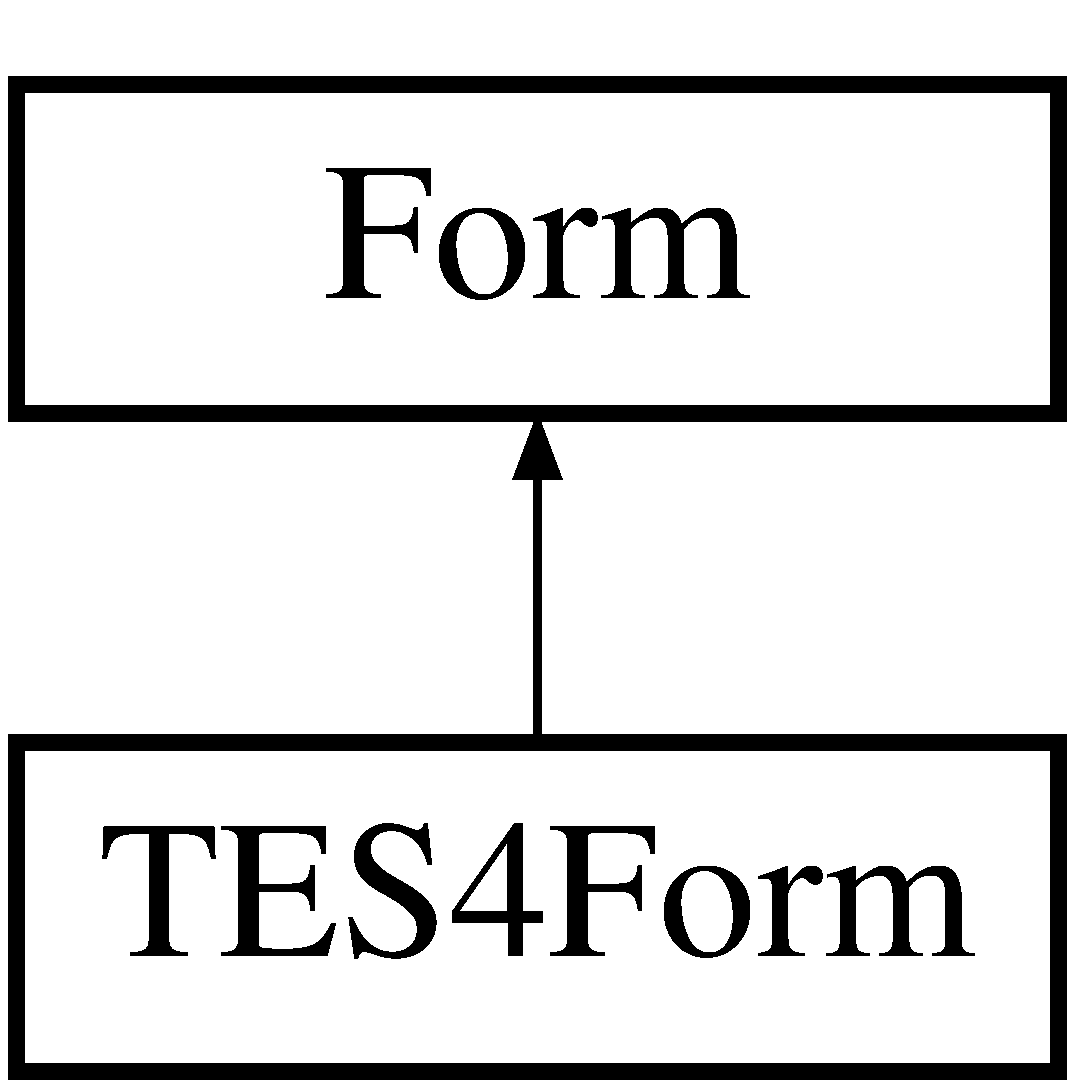
\includegraphics[height=2.000000cm]{class_form}
\end{center}
\end{figure}
\subsection*{Public Member Functions}
\begin{DoxyCompactItemize}
\item 
\hyperlink{class_form_a74d41f789dbfcfd081b241e2c44e576a}{Form} ()
\begin{DoxyCompactList}\small\item\em Constructs the \hyperlink{class_form}{Form} with default values of 0. \end{DoxyCompactList}\item 
\mbox{\Hypertarget{class_form_a4c68e6dfae9d8674fc9a55bfa9be34e3}\label{class_form_a4c68e6dfae9d8674fc9a55bfa9be34e3}} 
virtual void {\bfseries load} (Q\+Data\+Stream $\ast$in)=0
\end{DoxyCompactItemize}
\subsection*{Protected Attributes}
\begin{DoxyCompactItemize}
\item 
Form\+Name \hyperlink{class_form_a3a19912be281bc3e9c99911bb70e0f4b}{name}
\begin{DoxyCompactList}\small\item\em Name of the form. \end{DoxyCompactList}\item 
\hyperlink{struct_form_header}{Form\+Header} \hyperlink{class_form_a6aec4c07386c72bb12947f7766562856}{header}
\begin{DoxyCompactList}\small\item\em The form\textquotesingle{}s header. \end{DoxyCompactList}\end{DoxyCompactItemize}


\subsection{Detailed Description}
The base class for forms in .esp and .esm files. 

The abstract class that is the base for all parsed forms in .esp and .esm files. 

\subsection{Constructor \& Destructor Documentation}
\mbox{\Hypertarget{class_form_a74d41f789dbfcfd081b241e2c44e576a}\label{class_form_a74d41f789dbfcfd081b241e2c44e576a}} 
\index{Form@{Form}!Form@{Form}}
\index{Form@{Form}!Form@{Form}}
\subsubsection{\texorpdfstring{Form()}{Form()}}
{\footnotesize\ttfamily Form\+::\+Form (\begin{DoxyParamCaption}{ }\end{DoxyParamCaption})}



Constructs the \hyperlink{class_form}{Form} with default values of 0. 

Constructs the \hyperlink{class_form}{Form} object with the default values of 0. 

\subsection{Member Data Documentation}
\mbox{\Hypertarget{class_form_a6aec4c07386c72bb12947f7766562856}\label{class_form_a6aec4c07386c72bb12947f7766562856}} 
\index{Form@{Form}!header@{header}}
\index{header@{header}!Form@{Form}}
\subsubsection{\texorpdfstring{header}{header}}
{\footnotesize\ttfamily \hyperlink{struct_form_header}{Form\+Header} Form\+::header\hspace{0.3cm}{\ttfamily [protected]}}



The form\textquotesingle{}s header. 

The header of the form, with needed data for the parser. \mbox{\Hypertarget{class_form_a3a19912be281bc3e9c99911bb70e0f4b}\label{class_form_a3a19912be281bc3e9c99911bb70e0f4b}} 
\index{Form@{Form}!name@{name}}
\index{name@{name}!Form@{Form}}
\subsubsection{\texorpdfstring{name}{name}}
{\footnotesize\ttfamily Form\+Name Form\+::name\hspace{0.3cm}{\ttfamily [protected]}}



Name of the form. 

The name of the form. 

The documentation for this class was generated from the following files\+:\begin{DoxyCompactItemize}
\item 
C\+:/\+Users/alexa/\+Documents/\+Coding/\+Qt/why/openck/\+Open\+C\+K/include/define/form.\+h\item 
C\+:/\+Users/alexa/\+Documents/\+Coding/\+Qt/why/openck/\+Open\+C\+K/src/define/form.\+cpp\end{DoxyCompactItemize}

\hypertarget{struct_form_header}{}\section{Form\+Header Struct Reference}
\label{struct_form_header}\index{Form\+Header@{Form\+Header}}


The header of the nonparsed form.  




{\ttfamily \#include $<$form.\+h$>$}

\subsection*{Public Attributes}
\begin{DoxyCompactItemize}
\item 
uint32\+\_\+t \hyperlink{struct_form_header_a7c328abb1290000cef194ba4b71289db}{type}
\begin{DoxyCompactList}\small\item\em The type of the form in binary. \end{DoxyCompactList}\item 
uint32\+\_\+t \hyperlink{struct_form_header_a39628718fdb8e8825236f8d435bb723a}{data\+Size}
\begin{DoxyCompactList}\small\item\em The size of the data in the form. \end{DoxyCompactList}\item 
uint32\+\_\+t \hyperlink{struct_form_header_afdbca03050703e03f70e073ad1fda83f}{flags}
\begin{DoxyCompactList}\small\item\em The flags of the form. \end{DoxyCompactList}\item 
uint32\+\_\+t \hyperlink{struct_form_header_a848f4bb1320b2c08b8d865151ccd8ee3}{id}
\begin{DoxyCompactList}\small\item\em The form identifier. \end{DoxyCompactList}\item 
uint32\+\_\+t \hyperlink{struct_form_header_a32a8415135b878ae97078d696cf54e1e}{revision}
\begin{DoxyCompactList}\small\item\em The revision control id. \end{DoxyCompactList}\item 
uint32\+\_\+t \hyperlink{struct_form_header_a44d62c93920ca145bdfa363ee71b18aa}{version}
\begin{DoxyCompactList}\small\item\em The version of an unknown entity. \end{DoxyCompactList}\item 
uint16\+\_\+t \hyperlink{struct_form_header_aec53fee93e6738cbb7d95e74043337ac}{unknown}
\begin{DoxyCompactList}\small\item\em Unknown. \end{DoxyCompactList}\end{DoxyCompactItemize}


\subsection{Detailed Description}
The header of the nonparsed form. 

The header of the form which contains nonparsed needed information. 

\subsection{Member Data Documentation}
\mbox{\Hypertarget{struct_form_header_a39628718fdb8e8825236f8d435bb723a}\label{struct_form_header_a39628718fdb8e8825236f8d435bb723a}} 
\index{Form\+Header@{Form\+Header}!data\+Size@{data\+Size}}
\index{data\+Size@{data\+Size}!Form\+Header@{Form\+Header}}
\subsubsection{\texorpdfstring{data\+Size}{dataSize}}
{\footnotesize\ttfamily uint32\+\_\+t Form\+Header\+::data\+Size}



The size of the data in the form. 

The size of the data in the form, in bytes. \mbox{\Hypertarget{struct_form_header_afdbca03050703e03f70e073ad1fda83f}\label{struct_form_header_afdbca03050703e03f70e073ad1fda83f}} 
\index{Form\+Header@{Form\+Header}!flags@{flags}}
\index{flags@{flags}!Form\+Header@{Form\+Header}}
\subsubsection{\texorpdfstring{flags}{flags}}
{\footnotesize\ttfamily uint32\+\_\+t Form\+Header\+::flags}



The flags of the form. 

The flags (if any) of the form. \mbox{\Hypertarget{struct_form_header_a848f4bb1320b2c08b8d865151ccd8ee3}\label{struct_form_header_a848f4bb1320b2c08b8d865151ccd8ee3}} 
\index{Form\+Header@{Form\+Header}!id@{id}}
\index{id@{id}!Form\+Header@{Form\+Header}}
\subsubsection{\texorpdfstring{id}{id}}
{\footnotesize\ttfamily uint32\+\_\+t Form\+Header\+::id}



The form identifier. 

The form identifier. \mbox{\Hypertarget{struct_form_header_a32a8415135b878ae97078d696cf54e1e}\label{struct_form_header_a32a8415135b878ae97078d696cf54e1e}} 
\index{Form\+Header@{Form\+Header}!revision@{revision}}
\index{revision@{revision}!Form\+Header@{Form\+Header}}
\subsubsection{\texorpdfstring{revision}{revision}}
{\footnotesize\ttfamily uint32\+\_\+t Form\+Header\+::revision}



The revision control id. 

The id used for revision control. \mbox{\Hypertarget{struct_form_header_a7c328abb1290000cef194ba4b71289db}\label{struct_form_header_a7c328abb1290000cef194ba4b71289db}} 
\index{Form\+Header@{Form\+Header}!type@{type}}
\index{type@{type}!Form\+Header@{Form\+Header}}
\subsubsection{\texorpdfstring{type}{type}}
{\footnotesize\ttfamily uint32\+\_\+t Form\+Header\+::type}



The type of the form in binary. 

The type of the form. This will parse into a char\mbox{[}4\mbox{]} with each character being a Win1252 encoded byte. \mbox{\Hypertarget{struct_form_header_aec53fee93e6738cbb7d95e74043337ac}\label{struct_form_header_aec53fee93e6738cbb7d95e74043337ac}} 
\index{Form\+Header@{Form\+Header}!unknown@{unknown}}
\index{unknown@{unknown}!Form\+Header@{Form\+Header}}
\subsubsection{\texorpdfstring{unknown}{unknown}}
{\footnotesize\ttfamily uint16\+\_\+t Form\+Header\+::unknown}



Unknown. 

An unknown value, but it exists in the form header nonetheless. \mbox{\Hypertarget{struct_form_header_a44d62c93920ca145bdfa363ee71b18aa}\label{struct_form_header_a44d62c93920ca145bdfa363ee71b18aa}} 
\index{Form\+Header@{Form\+Header}!version@{version}}
\index{version@{version}!Form\+Header@{Form\+Header}}
\subsubsection{\texorpdfstring{version}{version}}
{\footnotesize\ttfamily uint32\+\_\+t Form\+Header\+::version}



The version of an unknown entity. 

The version of an unknown entity, but it exists in the form header nonetheless. 

The documentation for this struct was generated from the following file\+:\begin{DoxyCompactItemize}
\item 
C\+:/\+Users/alexa/\+Documents/\+Coding/\+Qt/why/openck/\+Open\+C\+K/include/define/form.\+h\end{DoxyCompactItemize}

\hypertarget{class_main_window}{}\section{Main\+Window Class Reference}
\label{class_main_window}\index{Main\+Window@{Main\+Window}}


The \hyperlink{class_main_window}{Main\+Window} class in the UI.  




{\ttfamily \#include $<$mainwindow.\+h$>$}

Inheritance diagram for Main\+Window\+:\begin{figure}[H]
\begin{center}
\leavevmode
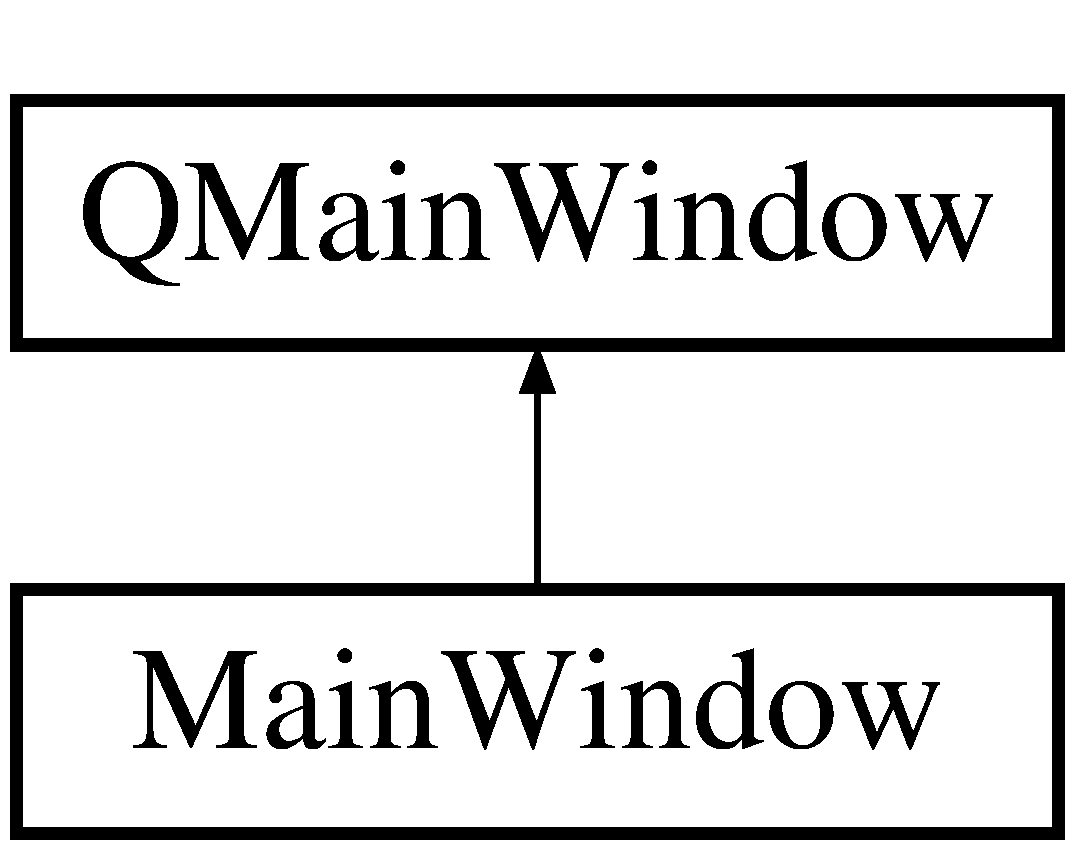
\includegraphics[height=2.000000cm]{class_main_window}
\end{center}
\end{figure}
\subsection*{Public Member Functions}
\begin{DoxyCompactItemize}
\item 
\hyperlink{class_main_window_a8b244be8b7b7db1b08de2a2acb9409db}{Main\+Window} (Q\+Widget $\ast$parent=0)
\begin{DoxyCompactList}\small\item\em Creates and sets up the Main Window. \end{DoxyCompactList}\item 
\hyperlink{class_main_window_ae98d00a93bc118200eeef9f9bba1dba7}{$\sim$\+Main\+Window} ()
\begin{DoxyCompactList}\small\item\em Destructs the main Window. \end{DoxyCompactList}\end{DoxyCompactItemize}
\subsection*{Private Slots}
\begin{DoxyCompactItemize}
\item 
void \hyperlink{class_main_window_a3ca9d4a4b5afe31afaff0d89a84c68fb}{on\+\_\+action\+Data\+\_\+triggered} ()
\begin{DoxyCompactList}\small\item\em Creates the data window. \end{DoxyCompactList}\item 
void \hyperlink{class_main_window_ad550c61cfa05c7e528dedc6cf636ed10}{on\+\_\+action\+Save\+\_\+triggered} ()
\begin{DoxyCompactList}\small\item\em \hyperlink{class_main_window_ad550c61cfa05c7e528dedc6cf636ed10}{Main\+Window\+::on\+\_\+action\+Save\+\_\+triggered()} \end{DoxyCompactList}\item 
void \hyperlink{class_main_window_a7df050ed9d3ca5f73a3ed852b35fc736}{on\+\_\+action\+Export\+\_\+triggered} ()
\begin{DoxyCompactList}\small\item\em \hyperlink{class_main_window_a7df050ed9d3ca5f73a3ed852b35fc736}{Main\+Window\+::on\+\_\+action\+Export\+\_\+triggered()} \end{DoxyCompactList}\item 
void \hyperlink{class_main_window_a2e63d199e37300ac181f39c3a7a7d78b}{on\+\_\+action\+Preferences\+\_\+triggered} ()
\begin{DoxyCompactList}\small\item\em \hyperlink{class_main_window_a2e63d199e37300ac181f39c3a7a7d78b}{Main\+Window\+::on\+\_\+action\+Preferences\+\_\+triggered()} \end{DoxyCompactList}\item 
void \hyperlink{class_main_window_ab1627fe6865e74d1e6364a0183abdf5c}{on\+\_\+action\+Validate\+\_\+\+Loaded\+\_\+\+Data\+\_\+triggered} ()
\begin{DoxyCompactList}\small\item\em \hyperlink{class_main_window_ab1627fe6865e74d1e6364a0183abdf5c}{Main\+Window\+::on\+\_\+action\+Validate\+\_\+\+Loaded\+\_\+\+Data\+\_\+triggered()} \end{DoxyCompactList}\item 
void \hyperlink{class_main_window_a6ac0bcf0b051abe049c84075e0a5d13a}{on\+\_\+action\+Create\+\_\+\+Archive\+\_\+triggered} ()
\begin{DoxyCompactList}\small\item\em \hyperlink{class_main_window_a6ac0bcf0b051abe049c84075e0a5d13a}{Main\+Window\+::on\+\_\+action\+Create\+\_\+\+Archive\+\_\+triggered()} \end{DoxyCompactList}\item 
void \hyperlink{class_main_window_a3e35b065b22cbe720c98787325b348c9}{on\+\_\+action\+Upload\+\_\+\+Active\+\_\+\+Plugin\+\_\+to\+\_\+\+Steam\+\_\+triggered} ()
\begin{DoxyCompactList}\small\item\em \hyperlink{class_main_window_a3e35b065b22cbe720c98787325b348c9}{Main\+Window\+::on\+\_\+action\+Upload\+\_\+\+Active\+\_\+\+Plugin\+\_\+to\+\_\+\+Steam\+\_\+triggered()} \end{DoxyCompactList}\item 
void \hyperlink{class_main_window_ab4487c4b02224acd4a0193d38b704ddb}{on\+\_\+action\+Exit\+\_\+triggered} ()
\begin{DoxyCompactList}\small\item\em Exits the application. \end{DoxyCompactList}\item 
void \hyperlink{class_main_window_abbab7cd8683132f28cf976d069c7c448}{on\+\_\+action\+Undo\+\_\+triggered} ()
\begin{DoxyCompactList}\small\item\em \hyperlink{class_main_window_abbab7cd8683132f28cf976d069c7c448}{Main\+Window\+::on\+\_\+action\+Undo\+\_\+triggered()} \end{DoxyCompactList}\item 
void \hyperlink{class_main_window_a386390413f5b36190ba30ab8d4c653d0}{on\+\_\+action\+Redo\+\_\+triggered} ()
\begin{DoxyCompactList}\small\item\em \hyperlink{class_main_window_a386390413f5b36190ba30ab8d4c653d0}{Main\+Window\+::on\+\_\+action\+Redo\+\_\+triggered()} \end{DoxyCompactList}\item 
void \hyperlink{class_main_window_aab15905e4c662653ff9e22457ab18964}{on\+\_\+action\+Cut\+\_\+\+Render\+\_\+triggered} ()
\begin{DoxyCompactList}\small\item\em \hyperlink{class_main_window_aab15905e4c662653ff9e22457ab18964}{Main\+Window\+::on\+\_\+action\+Cut\+\_\+\+Render\+\_\+triggered()} \end{DoxyCompactList}\item 
void \hyperlink{class_main_window_a5e9b919e05294457c7ea69f11afa0af8}{on\+\_\+action\+Copy\+\_\+\+Render\+\_\+triggered} ()
\begin{DoxyCompactList}\small\item\em \hyperlink{class_main_window_a5e9b919e05294457c7ea69f11afa0af8}{Main\+Window\+::on\+\_\+action\+Copy\+\_\+\+Render\+\_\+triggered()} \end{DoxyCompactList}\item 
void \hyperlink{class_main_window_a8587cd1f94682b6ac53b321b632e1220}{on\+\_\+action\+Paste\+\_\+\+Render\+\_\+triggered} ()
\begin{DoxyCompactList}\small\item\em \hyperlink{class_main_window_a8587cd1f94682b6ac53b321b632e1220}{Main\+Window\+::on\+\_\+action\+Paste\+\_\+\+Render\+\_\+triggered()} \end{DoxyCompactList}\item 
void \hyperlink{class_main_window_a675facd954ba9ceb4af6b3496a7db66e}{on\+\_\+action\+Paste\+\_\+in\+\_\+\+Place\+\_\+triggered} ()
\begin{DoxyCompactList}\small\item\em \hyperlink{class_main_window_a675facd954ba9ceb4af6b3496a7db66e}{Main\+Window\+::on\+\_\+action\+Paste\+\_\+in\+\_\+\+Place\+\_\+triggered()} \end{DoxyCompactList}\item 
void \hyperlink{class_main_window_af5060bd55fe1e9a7196be8a2dab1622e}{on\+\_\+action\+Duplicate\+\_\+triggered} ()
\begin{DoxyCompactList}\small\item\em \hyperlink{class_main_window_af5060bd55fe1e9a7196be8a2dab1622e}{Main\+Window\+::on\+\_\+action\+Duplicate\+\_\+triggered()} \end{DoxyCompactList}\item 
void \hyperlink{class_main_window_a8447eeb10a01419b396f470c0745ec01}{on\+\_\+action\+Search\+\_\+and\+\_\+\+Replace\+\_\+triggered} ()
\begin{DoxyCompactList}\small\item\em \hyperlink{class_main_window_a8447eeb10a01419b396f470c0745ec01}{Main\+Window\+::on\+\_\+action\+Search\+\_\+and\+\_\+\+Replace\+\_\+triggered()} \end{DoxyCompactList}\item 
void \hyperlink{class_main_window_a83f715fceb4ae6b29bc3dbf86260b580}{on\+\_\+action\+Find\+\_\+\+Text\+\_\+triggered} ()
\begin{DoxyCompactList}\small\item\em \hyperlink{class_main_window_a83f715fceb4ae6b29bc3dbf86260b580}{Main\+Window\+::on\+\_\+action\+Find\+\_\+\+Text\+\_\+triggered()} \end{DoxyCompactList}\item 
void \hyperlink{class_main_window_a06cab8e06cb83d2e79c4bdd0e0cd5a88}{on\+\_\+action\+Render\+\_\+\+Window\+\_\+\+Hotkeys\+\_\+triggered} ()
\begin{DoxyCompactList}\small\item\em \hyperlink{class_main_window_a06cab8e06cb83d2e79c4bdd0e0cd5a88}{Main\+Window\+::on\+\_\+action\+Render\+\_\+\+Window\+\_\+\+Hotkeys\+\_\+triggered()} \end{DoxyCompactList}\item 
void \hyperlink{class_main_window_a0361ab994394a05a31374b9e5b873d3b}{on\+\_\+action\+Render\+\_\+\+Window\+\_\+\+Preferences\+\_\+triggered} ()
\begin{DoxyCompactList}\small\item\em \hyperlink{class_main_window_a0361ab994394a05a31374b9e5b873d3b}{Main\+Window\+::on\+\_\+action\+Render\+\_\+\+Window\+\_\+\+Preferences\+\_\+triggered()} \end{DoxyCompactList}\item 
void \hyperlink{class_main_window_a0f037e29b645ecfd6a256136bfc1ee38}{on\+\_\+action\+Toolbar\+\_\+triggered} ()
\begin{DoxyCompactList}\small\item\em \hyperlink{class_main_window_a0f037e29b645ecfd6a256136bfc1ee38}{Main\+Window\+::on\+\_\+action\+Toolbar\+\_\+triggered()} \end{DoxyCompactList}\item 
void \hyperlink{class_main_window_a37848047e4bc8594a3e83e75bd6383cf}{on\+\_\+action\+Statusbar\+\_\+triggered} ()
\begin{DoxyCompactList}\small\item\em \hyperlink{class_main_window_a37848047e4bc8594a3e83e75bd6383cf}{Main\+Window\+::on\+\_\+action\+Statusbar\+\_\+triggered()} \end{DoxyCompactList}\item 
void \hyperlink{class_main_window_a60eede6fe328bc95cccfe0c6d4a7696e}{on\+\_\+action\+Open\+\_\+\+Windows\+\_\+triggered} ()
\begin{DoxyCompactList}\small\item\em \hyperlink{class_main_window_a60eede6fe328bc95cccfe0c6d4a7696e}{Main\+Window\+::on\+\_\+action\+Open\+\_\+\+Windows\+\_\+triggered()} \end{DoxyCompactList}\item 
void \hyperlink{class_main_window_a584ef402e75f991b95af6dadbaac6354}{on\+\_\+action\+Object\+\_\+\+Window\+\_\+triggered} ()
\begin{DoxyCompactList}\small\item\em \hyperlink{class_main_window_a584ef402e75f991b95af6dadbaac6354}{Main\+Window\+::on\+\_\+action\+Object\+\_\+\+Window\+\_\+triggered()} \end{DoxyCompactList}\item 
void \hyperlink{class_main_window_acca897b6aa864947f35e22163eb6a0a7}{on\+\_\+action\+Cell\+\_\+\+View\+\_\+\+Window\+\_\+triggered} ()
\begin{DoxyCompactList}\small\item\em \hyperlink{class_main_window_acca897b6aa864947f35e22163eb6a0a7}{Main\+Window\+::on\+\_\+action\+Cell\+\_\+\+View\+\_\+\+Window\+\_\+triggered()} \end{DoxyCompactList}\item 
void \hyperlink{class_main_window_a5e8eef1130ab17d4f10ae161eb372bc8}{on\+\_\+action\+Scene\+\_\+\+Info\+\_\+\+Window\+\_\+triggered} ()
\begin{DoxyCompactList}\small\item\em \hyperlink{class_main_window_a5e8eef1130ab17d4f10ae161eb372bc8}{Main\+Window\+::on\+\_\+action\+Scene\+\_\+\+Info\+\_\+\+Window\+\_\+triggered()} \end{DoxyCompactList}\item 
void \hyperlink{class_main_window_ad39efdb57cad0ee03b2491037fa6b5c0}{on\+\_\+action\+Preview\+\_\+\+Window\+\_\+triggered} ()
\begin{DoxyCompactList}\small\item\em \hyperlink{class_main_window_ad39efdb57cad0ee03b2491037fa6b5c0}{Main\+Window\+::on\+\_\+action\+Preview\+\_\+\+Window\+\_\+triggered()} \end{DoxyCompactList}\item 
void \hyperlink{class_main_window_a3de1a7a9eb5798b608bdb9fad1a442b5}{on\+\_\+action\+Show\+\_\+\+Hide\+\_\+\+Window\+\_\+triggered} ()
\begin{DoxyCompactList}\small\item\em \hyperlink{class_main_window_a3de1a7a9eb5798b608bdb9fad1a442b5}{Main\+Window\+::on\+\_\+action\+Show\+\_\+\+Hide\+\_\+\+Window\+\_\+triggered()} \end{DoxyCompactList}\item 
void \hyperlink{class_main_window_a162cfcb7e13f7d350c9246e2a084eb6b}{on\+\_\+action\+Reference\+\_\+\+Batch\+\_\+\+Action\+\_\+\+Window\+\_\+triggered} ()
\begin{DoxyCompactList}\small\item\em \hyperlink{class_main_window_a162cfcb7e13f7d350c9246e2a084eb6b}{Main\+Window\+::on\+\_\+action\+Reference\+\_\+\+Batch\+\_\+\+Action\+\_\+\+Window\+\_\+triggered()} \end{DoxyCompactList}\item 
void \hyperlink{class_main_window_a58acaabf35d71b094d373c5a8f4f333a}{on\+\_\+action\+Current\+\_\+\+Cell\+\_\+\+Only\+\_\+triggered} ()
\begin{DoxyCompactList}\small\item\em \hyperlink{class_main_window_a58acaabf35d71b094d373c5a8f4f333a}{Main\+Window\+::on\+\_\+action\+Current\+\_\+\+Cell\+\_\+\+Only\+\_\+triggered()} \end{DoxyCompactList}\item 
void \hyperlink{class_main_window_addae5ed0b02101880ff1907c4b2c5864}{on\+\_\+action\+Markers\+\_\+triggered} ()
\begin{DoxyCompactList}\small\item\em \hyperlink{class_main_window_addae5ed0b02101880ff1907c4b2c5864}{Main\+Window\+::on\+\_\+action\+Markers\+\_\+triggered()} \end{DoxyCompactList}\item 
void \hyperlink{class_main_window_a761bc0d259399f5ddb9df53b0435e1d9}{on\+\_\+action\+Light\+\_\+\+Markers\+\_\+triggered} ()
\begin{DoxyCompactList}\small\item\em \hyperlink{class_main_window_a761bc0d259399f5ddb9df53b0435e1d9}{Main\+Window\+::on\+\_\+action\+Light\+\_\+\+Markers\+\_\+triggered()} \end{DoxyCompactList}\item 
void \hyperlink{class_main_window_a4b49e5d0db6f503d31748bf48c3179e7}{on\+\_\+action\+Sound\+\_\+\+Markers\+\_\+triggered} ()
\begin{DoxyCompactList}\small\item\em \hyperlink{class_main_window_a4b49e5d0db6f503d31748bf48c3179e7}{Main\+Window\+::on\+\_\+action\+Sound\+\_\+\+Markers\+\_\+triggered()} \end{DoxyCompactList}\item 
void \hyperlink{class_main_window_a05175ca29c0d327277b1642d1e974e66}{on\+\_\+action\+Light\+\_\+\+Radius\+\_\+triggered} ()
\begin{DoxyCompactList}\small\item\em \hyperlink{class_main_window_a05175ca29c0d327277b1642d1e974e66}{Main\+Window\+::on\+\_\+action\+Light\+\_\+\+Radius\+\_\+triggered()} \end{DoxyCompactList}\item 
void \hyperlink{class_main_window_a96b669e857f9f600d938cc735632da04}{on\+\_\+action\+Wireframe\+\_\+triggered} ()
\begin{DoxyCompactList}\small\item\em \hyperlink{class_main_window_a96b669e857f9f600d938cc735632da04}{Main\+Window\+::on\+\_\+action\+Wireframe\+\_\+triggered()} \end{DoxyCompactList}\item 
void \hyperlink{class_main_window_aa4301fd4cad1597fad079ee7eebbd14a}{on\+\_\+action\+Sky\+\_\+triggered} ()
\begin{DoxyCompactList}\small\item\em \hyperlink{class_main_window_aa4301fd4cad1597fad079ee7eebbd14a}{Main\+Window\+::on\+\_\+action\+Sky\+\_\+triggered()} \end{DoxyCompactList}\item 
void \hyperlink{class_main_window_ac2ff07ecfb39bbcd9f863693bd3bb146}{on\+\_\+action\+Grass\+\_\+triggered} ()
\begin{DoxyCompactList}\small\item\em \hyperlink{class_main_window_ac2ff07ecfb39bbcd9f863693bd3bb146}{Main\+Window\+::on\+\_\+action\+Grass\+\_\+triggered()} \end{DoxyCompactList}\item 
void \hyperlink{class_main_window_af815e187182d6f7ccfb7264814a128f9}{on\+\_\+action\+Fog\+\_\+triggered} ()
\begin{DoxyCompactList}\small\item\em \hyperlink{class_main_window_af815e187182d6f7ccfb7264814a128f9}{Main\+Window\+::on\+\_\+action\+Fog\+\_\+triggered()} \end{DoxyCompactList}\item 
void \hyperlink{class_main_window_a6ef9945ba6ef944e564436d94b643c1c}{on\+\_\+action\+Leaves\+\_\+triggered} ()
\begin{DoxyCompactList}\small\item\em \hyperlink{class_main_window_a6ef9945ba6ef944e564436d94b643c1c}{Main\+Window\+::on\+\_\+action\+Leaves\+\_\+triggered()} \end{DoxyCompactList}\item 
void \hyperlink{class_main_window_ab29f6867e27f4f7bbb30eb31d7a152d2}{on\+\_\+action\+Trees\+\_\+triggered} ()
\begin{DoxyCompactList}\small\item\em \hyperlink{class_main_window_ab29f6867e27f4f7bbb30eb31d7a152d2}{Main\+Window\+::on\+\_\+action\+Trees\+\_\+triggered()} \end{DoxyCompactList}\item 
void \hyperlink{class_main_window_a26f1dd43b9b49ddc65d8e6a0ab7f2b6b}{on\+\_\+action\+Collision\+\_\+\+Geometry\+\_\+triggered} ()
\begin{DoxyCompactList}\small\item\em \hyperlink{class_main_window_a26f1dd43b9b49ddc65d8e6a0ab7f2b6b}{Main\+Window\+::on\+\_\+action\+Collision\+\_\+\+Geometry\+\_\+triggered()} \end{DoxyCompactList}\item 
void \hyperlink{class_main_window_a5276a8a1574c6344dbf4e2151caf0a08}{on\+\_\+action\+Occlusion\+\_\+\+Planes\+\_\+triggered} ()
\begin{DoxyCompactList}\small\item\em \hyperlink{class_main_window_a5276a8a1574c6344dbf4e2151caf0a08}{Main\+Window\+::on\+\_\+action\+Occlusion\+\_\+\+Planes\+\_\+triggered()} \end{DoxyCompactList}\item 
void \hyperlink{class_main_window_a9a1c4d7a462288215d815f7b6c87f7c1}{on\+\_\+action\+Isometric\+\_\+triggered} ()
\begin{DoxyCompactList}\small\item\em \hyperlink{class_main_window_a9a1c4d7a462288215d815f7b6c87f7c1}{Main\+Window\+::on\+\_\+action\+Isometric\+\_\+triggered()} \end{DoxyCompactList}\item 
void \hyperlink{class_main_window_a12c196357f488415909efd293a2bf6d0}{on\+\_\+action\+Top\+\_\+triggered} ()
\begin{DoxyCompactList}\small\item\em \hyperlink{class_main_window_a12c196357f488415909efd293a2bf6d0}{Main\+Window\+::on\+\_\+action\+Top\+\_\+triggered()} \end{DoxyCompactList}\item 
void \hyperlink{class_main_window_a85f9b158b4cf913593135ac5b3321b81}{on\+\_\+action\+Depth\+\_\+\+Biasing\+\_\+triggered} ()
\begin{DoxyCompactList}\small\item\em \hyperlink{class_main_window_a85f9b158b4cf913593135ac5b3321b81}{Main\+Window\+::on\+\_\+action\+Depth\+\_\+\+Biasing\+\_\+triggered()} \end{DoxyCompactList}\item 
void \hyperlink{class_main_window_a52c7776d665150af7b2393ab3e72b8d6}{on\+\_\+action\+Refresh\+\_\+\+Render\+\_\+\+Window\+\_\+triggered} ()
\begin{DoxyCompactList}\small\item\em \hyperlink{class_main_window_a52c7776d665150af7b2393ab3e72b8d6}{Main\+Window\+::on\+\_\+action\+Refresh\+\_\+\+Render\+\_\+\+Window\+\_\+triggered()} \end{DoxyCompactList}\item 
void \hyperlink{class_main_window_a018b6c693a863ad693ae5c5711e7e9a0}{on\+\_\+action\+Warnings\+\_\+triggered} ()
\begin{DoxyCompactList}\small\item\em \hyperlink{class_main_window_a018b6c693a863ad693ae5c5711e7e9a0}{Main\+Window\+::on\+\_\+action\+Warnings\+\_\+triggered()} \end{DoxyCompactList}\item 
void \hyperlink{class_main_window_a8e0b3c4ebbe0e6a744500f32e7b343f9}{on\+\_\+action\+World\+\_\+\+Spaces\+\_\+triggered} ()
\begin{DoxyCompactList}\small\item\em \hyperlink{class_main_window_a8e0b3c4ebbe0e6a744500f32e7b343f9}{Main\+Window\+::on\+\_\+action\+World\+\_\+\+Spaces\+\_\+triggered()} \end{DoxyCompactList}\item 
void \hyperlink{class_main_window_a4eae54da532473a41d4047cddca1adba}{on\+\_\+action\+Regions\+\_\+triggered} ()
\begin{DoxyCompactList}\small\item\em \hyperlink{class_main_window_a4eae54da532473a41d4047cddca1adba}{Main\+Window\+::on\+\_\+action\+Regions\+\_\+triggered()} \end{DoxyCompactList}\item 
void \hyperlink{class_main_window_abe162b3673599552213251a049a93eac}{on\+\_\+action\+Cells\+\_\+triggered} ()
\begin{DoxyCompactList}\small\item\em \hyperlink{class_main_window_abe162b3673599552213251a049a93eac}{Main\+Window\+::on\+\_\+action\+Cells\+\_\+triggered()} \end{DoxyCompactList}\item 
void \hyperlink{class_main_window_ac8f6bda78b3a005a294a7a1304acd1ec}{on\+\_\+action\+World\+\_\+\+L\+O\+D\+\_\+triggered} ()
\begin{DoxyCompactList}\small\item\em \hyperlink{class_main_window_ac8f6bda78b3a005a294a7a1304acd1ec}{Main\+Window\+::on\+\_\+action\+World\+\_\+\+L\+O\+D\+\_\+triggered()} \end{DoxyCompactList}\item 
void \hyperlink{class_main_window_ad66df2de0ccf574f449f5e7258bcdfba}{on\+\_\+action\+T\+O\+D\+O\+\_\+triggered} ()
\begin{DoxyCompactList}\small\item\em \hyperlink{class_main_window_ad66df2de0ccf574f449f5e7258bcdfba}{Main\+Window\+::on\+\_\+action\+T\+O\+D\+O\+\_\+triggered()} \end{DoxyCompactList}\item 
void \hyperlink{class_main_window_a772b1c26a74f70f9ecbe3348926cdd2c}{on\+\_\+action\+Test\+\_\+\+Icons\+\_\+\+Textures\+\_\+triggered} ()
\begin{DoxyCompactList}\small\item\em \hyperlink{class_main_window_a772b1c26a74f70f9ecbe3348926cdd2c}{Main\+Window\+::on\+\_\+action\+Test\+\_\+\+Icons\+\_\+\+Textures\+\_\+triggered()} \end{DoxyCompactList}\item 
void \hyperlink{class_main_window_a7ba69db7e0da3b95a98c3207deaabacb}{on\+\_\+action\+Test\+\_\+\+All\+\_\+\+Cells\+\_\+triggered} ()
\begin{DoxyCompactList}\small\item\em \hyperlink{class_main_window_a7ba69db7e0da3b95a98c3207deaabacb}{Main\+Window\+::on\+\_\+action\+Test\+\_\+\+All\+\_\+\+Cells\+\_\+triggered()} \end{DoxyCompactList}\item 
void \hyperlink{class_main_window_af1dd399ccee2cf368432256a4c8cfc36}{on\+\_\+action\+Test\+\_\+\+Interior\+\_\+\+Cells\+\_\+triggered} ()
\begin{DoxyCompactList}\small\item\em \hyperlink{class_main_window_af1dd399ccee2cf368432256a4c8cfc36}{Main\+Window\+::on\+\_\+action\+Test\+\_\+\+Interior\+\_\+\+Cells\+\_\+triggered()} \end{DoxyCompactList}\item 
void \hyperlink{class_main_window_a9f15c0cb032a4c6914806b0feac5ff9d}{on\+\_\+action\+Output\+\_\+\+Model\+\_\+\+Size\+\_\+\+List\+\_\+triggered} ()
\begin{DoxyCompactList}\small\item\em \hyperlink{class_main_window_a9f15c0cb032a4c6914806b0feac5ff9d}{Main\+Window\+::on\+\_\+action\+Output\+\_\+\+Model\+\_\+\+Size\+\_\+\+List\+\_\+triggered()} \end{DoxyCompactList}\item 
void \hyperlink{class_main_window_a0ffc9518de23f6fcc4b60286e5d70260}{on\+\_\+action\+View\+\_\+\+Render\+\_\+\+Test\+\_\+\+Failures\+\_\+triggered} ()
\begin{DoxyCompactList}\small\item\em \hyperlink{class_main_window_a0ffc9518de23f6fcc4b60286e5d70260}{Main\+Window\+::on\+\_\+action\+View\+\_\+\+Render\+\_\+\+Test\+\_\+\+Failures\+\_\+triggered()} \end{DoxyCompactList}\item 
void \hyperlink{class_main_window_a18145ab0d7747c6315778992ea38615a}{on\+\_\+action\+View\+\_\+\+Beta\+Comment\+\_\+\+Data\+\_\+triggered} ()
\begin{DoxyCompactList}\small\item\em \hyperlink{class_main_window_a18145ab0d7747c6315778992ea38615a}{Main\+Window\+::on\+\_\+action\+View\+\_\+\+Beta\+Comment\+\_\+\+Data\+\_\+triggered()} \end{DoxyCompactList}\item 
void \hyperlink{class_main_window_ac9c08be5071382e5c549eaa3d5d9ccaf}{on\+\_\+action\+Run\+\_\+\+Havok\+\_\+\+Sim\+\_\+triggered} ()
\begin{DoxyCompactList}\small\item\em \hyperlink{class_main_window_ac9c08be5071382e5c549eaa3d5d9ccaf}{Main\+Window\+::on\+\_\+action\+Run\+\_\+\+Havok\+\_\+\+Sim\+\_\+triggered()} \end{DoxyCompactList}\item 
void \hyperlink{class_main_window_a8d9c1bfde135eb7efac2eeeefa0178c0}{on\+\_\+action\+Update\+\_\+\+Lighting\+\_\+and\+\_\+\+Effects\+\_\+triggered} ()
\begin{DoxyCompactList}\small\item\em \hyperlink{class_main_window_a8d9c1bfde135eb7efac2eeeefa0178c0}{Main\+Window\+::on\+\_\+action\+Update\+\_\+\+Lighting\+\_\+and\+\_\+\+Effects\+\_\+triggered()} \end{DoxyCompactList}\item 
void \hyperlink{class_main_window_a80757bcc5466819ce28ceb0e7840a2eb}{on\+\_\+action\+Landscape\+\_\+\+Editing\+\_\+triggered} ()
\begin{DoxyCompactList}\small\item\em \hyperlink{class_main_window_a80757bcc5466819ce28ceb0e7840a2eb}{Main\+Window\+::on\+\_\+action\+Landscape\+\_\+\+Editing\+\_\+triggered()} \end{DoxyCompactList}\item 
void \hyperlink{class_main_window_a730870f9625a5a193dcb54d0e757301a}{on\+\_\+action\+Object\+\_\+\+Palette\+\_\+\+Editing\+\_\+triggered} ()
\begin{DoxyCompactList}\small\item\em \hyperlink{class_main_window_a730870f9625a5a193dcb54d0e757301a}{Main\+Window\+::on\+\_\+action\+Object\+\_\+\+Palette\+\_\+\+Editing\+\_\+triggered()} \end{DoxyCompactList}\item 
void \hyperlink{class_main_window_a5a0e9a546c0ccf99df38eabe7a51bcf9}{on\+\_\+action\+Heightmap\+\_\+\+Editing\+\_\+triggered} ()
\begin{DoxyCompactList}\small\item\em \hyperlink{class_main_window_a5a0e9a546c0ccf99df38eabe7a51bcf9}{Main\+Window\+::on\+\_\+action\+Heightmap\+\_\+\+Editing\+\_\+triggered()} \end{DoxyCompactList}\item 
void \hyperlink{class_main_window_a8ef4f1be069a5526d6d5f1aced12b5c3}{on\+\_\+action\+Create\+\_\+\+Local\+\_\+\+Maps\+\_\+triggered} ()
\begin{DoxyCompactList}\small\item\em \hyperlink{class_main_window_a8ef4f1be069a5526d6d5f1aced12b5c3}{Main\+Window\+::on\+\_\+action\+Create\+\_\+\+Local\+\_\+\+Maps\+\_\+triggered()} \end{DoxyCompactList}\item 
void \hyperlink{class_main_window_a8d9f011472c3ef05a97ee728f1ed8134}{on\+\_\+action\+Validate\+\_\+\+Room\+\_\+\+Portal\+\_\+\+Alignment\+\_\+triggered} ()
\begin{DoxyCompactList}\small\item\em \hyperlink{class_main_window_a8d9f011472c3ef05a97ee728f1ed8134}{Main\+Window\+::on\+\_\+action\+Validate\+\_\+\+Room\+\_\+\+Portal\+\_\+\+Alignment\+\_\+triggered()} \end{DoxyCompactList}\item 
void \hyperlink{class_main_window_a86bd042548f5e84c516b90d6d8b497ef}{on\+\_\+action\+Align\+\_\+\+Tangent\+\_\+\+Space\+\_\+at\+\_\+\+N\+I\+F\+\_\+\+Intersection\+\_\+triggered} ()
\begin{DoxyCompactList}\small\item\em \hyperlink{class_main_window_a86bd042548f5e84c516b90d6d8b497ef}{Main\+Window\+::on\+\_\+action\+Align\+\_\+\+Tangent\+\_\+\+Space\+\_\+at\+\_\+\+N\+I\+F\+\_\+\+Intersection\+\_\+triggered()} \end{DoxyCompactList}\item 
void \hyperlink{class_main_window_a3710309f29e6b68d71991f67bb29b069}{on\+\_\+action\+Generate\+\_\+\+L\+O\+S\+\_\+triggered} ()
\begin{DoxyCompactList}\small\item\em \hyperlink{class_main_window_a3710309f29e6b68d71991f67bb29b069}{Main\+Window\+::on\+\_\+action\+Generate\+\_\+\+L\+O\+S\+\_\+triggered()} \end{DoxyCompactList}\item 
void \hyperlink{class_main_window_abdad9bfc636dbe25f777c4c822ef9c37}{on\+\_\+action\+Generate\+\_\+\+Max\+\_\+\+Height\+\_\+\+Data\+\_\+\+For\+\_\+\+Current\+\_\+\+Cell\+\_\+triggered} ()
\begin{DoxyCompactList}\small\item\em \hyperlink{class_main_window_abdad9bfc636dbe25f777c4c822ef9c37}{Main\+Window\+::on\+\_\+action\+Generate\+\_\+\+Max\+\_\+\+Height\+\_\+\+Data\+\_\+\+For\+\_\+\+Current\+\_\+\+Cell\+\_\+triggered()} \end{DoxyCompactList}\item 
void \hyperlink{class_main_window_af239e60413e6c76eb2dcf61cb088e30a}{on\+\_\+action\+Generate\+\_\+\+Max\+\_\+\+Height\+\_\+\+Data\+\_\+\+For\+\_\+\+World\+\_\+triggered} ()
\begin{DoxyCompactList}\small\item\em \hyperlink{class_main_window_af239e60413e6c76eb2dcf61cb088e30a}{Main\+Window\+::on\+\_\+action\+Generate\+\_\+\+Max\+\_\+\+Height\+\_\+\+Data\+\_\+\+For\+\_\+\+World\+\_\+triggered()} \end{DoxyCompactList}\item 
void \hyperlink{class_main_window_a9075d8b9ba0b1304260baf359961fd15}{on\+\_\+action\+Generate\+\_\+\+Max\+\_\+\+Height\+\_\+\+Data\+\_\+\+For\+\_\+\+A\+L\+L\+\_\+\+Worlds\+\_\+triggered} ()
\begin{DoxyCompactList}\small\item\em \hyperlink{class_main_window_a9075d8b9ba0b1304260baf359961fd15}{Main\+Window\+::on\+\_\+action\+Generate\+\_\+\+Max\+\_\+\+Height\+\_\+\+Data\+\_\+\+For\+\_\+\+A\+L\+L\+\_\+\+Worlds\+\_\+triggered()} \end{DoxyCompactList}\item 
void \hyperlink{class_main_window_a8a36e600870d52f9610f71b81f0cda1c}{on\+\_\+action\+Object\+\_\+\+Based\+\_\+\+Generation\+\_\+triggered} ()
\begin{DoxyCompactList}\small\item\em \hyperlink{class_main_window_a8a36e600870d52f9610f71b81f0cda1c}{Main\+Window\+::on\+\_\+action\+Object\+\_\+\+Based\+\_\+\+Generation\+\_\+triggered()} \end{DoxyCompactList}\item 
void \hyperlink{class_main_window_acce573c1ebbc822a6008c05377a4f431}{on\+\_\+action\+Havok\+\_\+\+Based\+\_\+\+Generation\+\_\+triggered} ()
\begin{DoxyCompactList}\small\item\em \hyperlink{class_main_window_acce573c1ebbc822a6008c05377a4f431}{Main\+Window\+::on\+\_\+action\+Havok\+\_\+\+Based\+\_\+\+Generation\+\_\+triggered()} \end{DoxyCompactList}\item 
void \hyperlink{class_main_window_ab934ee7c4d674c16347171a4651765f9}{on\+\_\+action\+Recast\+\_\+\+Based\+\_\+\+Generation\+\_\+triggered} ()
\begin{DoxyCompactList}\small\item\em \hyperlink{class_main_window_ab934ee7c4d674c16347171a4651765f9}{Main\+Window\+::on\+\_\+action\+Recast\+\_\+\+Based\+\_\+\+Generation\+\_\+triggered()} \end{DoxyCompactList}\item 
void \hyperlink{class_main_window_a5aa2fcd339d653b805dd629bc5ada6ea}{on\+\_\+action\+Advanced\+\_\+triggered} ()
\begin{DoxyCompactList}\small\item\em \hyperlink{class_main_window_a5aa2fcd339d653b805dd629bc5ada6ea}{Main\+Window\+::on\+\_\+action\+Advanced\+\_\+triggered()} \end{DoxyCompactList}\item 
void \hyperlink{class_main_window_a967d58b1c44e2c438b3d1387852856f1}{on\+\_\+action\+Auto\+\_\+\+Generate\+\_\+\+World\+Space\+\_\+triggered} ()
\begin{DoxyCompactList}\small\item\em \hyperlink{class_main_window_a967d58b1c44e2c438b3d1387852856f1}{Main\+Window\+::on\+\_\+action\+Auto\+\_\+\+Generate\+\_\+\+World\+Space\+\_\+triggered()} \end{DoxyCompactList}\item 
void \hyperlink{class_main_window_a7b839044120c99de319e916b3804423d}{on\+\_\+action\+Check\+\_\+\+Nav\+Meshes\+\_\+triggered} ()
\begin{DoxyCompactList}\small\item\em \hyperlink{class_main_window_a7b839044120c99de319e916b3804423d}{Main\+Window\+::on\+\_\+action\+Check\+\_\+\+Nav\+Meshes\+\_\+triggered()} \end{DoxyCompactList}\item 
void \hyperlink{class_main_window_ac6952d7d9fe31aa25e570b898eb5257d}{on\+\_\+action\+Finalize\+\_\+\+Cell\+\_\+\+Nav\+Meshes\+\_\+triggered} ()
\begin{DoxyCompactList}\small\item\em \hyperlink{class_main_window_ac6952d7d9fe31aa25e570b898eb5257d}{Main\+Window\+::on\+\_\+action\+Finalize\+\_\+\+Cell\+\_\+\+Nav\+Meshes\+\_\+triggered()} \end{DoxyCompactList}\item 
void \hyperlink{class_main_window_a23fdbcb0c33b6f6327cffa6d2debf1ed}{on\+\_\+action\+Find\+\_\+\+Cover\+\_\+\+Edges\+\_\+triggered} ()
\begin{DoxyCompactList}\small\item\em \hyperlink{class_main_window_a23fdbcb0c33b6f6327cffa6d2debf1ed}{Main\+Window\+::on\+\_\+action\+Find\+\_\+\+Cover\+\_\+\+Edges\+\_\+triggered()} \end{DoxyCompactList}\item 
void \hyperlink{class_main_window_a22f2240480e250819d2fbbaf2a6cf13b}{on\+\_\+action\+Move\+\_\+\+Selection\+\_\+to\+\_\+\+Separate\+\_\+\+Nav\+Mesh\+\_\+triggered} ()
\begin{DoxyCompactList}\small\item\em \hyperlink{class_main_window_a22f2240480e250819d2fbbaf2a6cf13b}{Main\+Window\+::on\+\_\+action\+Move\+\_\+\+Selection\+\_\+to\+\_\+\+Separate\+\_\+\+Nav\+Mesh\+\_\+triggered()} \end{DoxyCompactList}\item 
void \hyperlink{class_main_window_ae9c6d0a50e7481bb627e9602b306a265}{on\+\_\+action\+Nav\+Mesh\+\_\+\+Draw\+\_\+\+Mode\+\_\+triggered} ()
\begin{DoxyCompactList}\small\item\em \hyperlink{class_main_window_ae9c6d0a50e7481bb627e9602b306a265}{Main\+Window\+::on\+\_\+action\+Nav\+Mesh\+\_\+\+Draw\+\_\+\+Mode\+\_\+triggered()} \end{DoxyCompactList}\item 
void \hyperlink{class_main_window_a95505aa506e45dc84d8890778ad64212}{on\+\_\+action\+Draw\+\_\+\+Cover\+\_\+triggered} ()
\begin{DoxyCompactList}\small\item\em \hyperlink{class_main_window_a95505aa506e45dc84d8890778ad64212}{Main\+Window\+::on\+\_\+action\+Draw\+\_\+\+Cover\+\_\+triggered()} \end{DoxyCompactList}\item 
void \hyperlink{class_main_window_a1c13e2deb928b26279035e49ffb5a381}{on\+\_\+action\+Clear\+\_\+\+Generated\+\_\+\+Cover\+\_\+triggered} ()
\begin{DoxyCompactList}\small\item\em \hyperlink{class_main_window_a1c13e2deb928b26279035e49ffb5a381}{Main\+Window\+::on\+\_\+action\+Clear\+\_\+\+Generated\+\_\+\+Cover\+\_\+triggered()} \end{DoxyCompactList}\item 
void \hyperlink{class_main_window_aa76285613d70d8f605af173f444232aa}{on\+\_\+action\+Clear\+\_\+\+Cover\+\_\+triggered} ()
\begin{DoxyCompactList}\small\item\em \hyperlink{class_main_window_aa76285613d70d8f605af173f444232aa}{Main\+Window\+::on\+\_\+action\+Clear\+\_\+\+Cover\+\_\+triggered()} \end{DoxyCompactList}\item 
void \hyperlink{class_main_window_a263f139f0eb0fe0f0986c71509a371f6}{on\+\_\+action\+Remove\+\_\+\+Cell\+\_\+\+Nav\+Meshes\+\_\+triggered} ()
\begin{DoxyCompactList}\small\item\em \hyperlink{class_main_window_a263f139f0eb0fe0f0986c71509a371f6}{Main\+Window\+::on\+\_\+action\+Remove\+\_\+\+Cell\+\_\+\+Nav\+Meshes\+\_\+triggered()} \end{DoxyCompactList}\item 
void \hyperlink{class_main_window_aa95e768258ffcd2b4d8f2460e620f9db}{on\+\_\+action\+Check\+\_\+\+World\+Space\+\_\+\+Cells\+\_\+for\+\_\+\+Finalize\+\_\+triggered} ()
\begin{DoxyCompactList}\small\item\em \hyperlink{class_main_window_aa95e768258ffcd2b4d8f2460e620f9db}{Main\+Window\+::on\+\_\+action\+Check\+\_\+\+World\+Space\+\_\+\+Cells\+\_\+for\+\_\+\+Finalize\+\_\+triggered()} \end{DoxyCompactList}\item 
void \hyperlink{class_main_window_a583a8bf84d1bde5fcf6af19accaa625c}{on\+\_\+action\+Finalize\+\_\+\+World\+Space\+\_\+triggered} ()
\begin{DoxyCompactList}\small\item\em \hyperlink{class_main_window_a583a8bf84d1bde5fcf6af19accaa625c}{Main\+Window\+::on\+\_\+action\+Finalize\+\_\+\+World\+Space\+\_\+triggered()} \end{DoxyCompactList}\item 
void \hyperlink{class_main_window_a39ce027d7a98f94efdb5dce1204c6b76}{on\+\_\+action\+Force\+\_\+\+Finalize\+\_\+\+Full\+\_\+\+World\+Space\+\_\+triggered} ()
\begin{DoxyCompactList}\small\item\em \hyperlink{class_main_window_a39ce027d7a98f94efdb5dce1204c6b76}{Main\+Window\+::on\+\_\+action\+Force\+\_\+\+Finalize\+\_\+\+Full\+\_\+\+World\+Space\+\_\+triggered()} \end{DoxyCompactList}\item 
void \hyperlink{class_main_window_a0976f59dc5b7864ab50343653dfc48ac}{on\+\_\+action\+Finalize\+\_\+\+All\+\_\+\+Interiors\+\_\+triggered} ()
\begin{DoxyCompactList}\small\item\em \hyperlink{class_main_window_a0976f59dc5b7864ab50343653dfc48ac}{Main\+Window\+::on\+\_\+action\+Finalize\+\_\+\+All\+\_\+\+Interiors\+\_\+triggered()} \end{DoxyCompactList}\item 
void \hyperlink{class_main_window_a2ac15d9b187bae1395956be2636bf84b}{on\+\_\+action\+Force\+\_\+\+Finalize\+\_\+\+All\+\_\+\+Spaces\+\_\+triggered} ()
\begin{DoxyCompactList}\small\item\em \hyperlink{class_main_window_a2ac15d9b187bae1395956be2636bf84b}{Main\+Window\+::on\+\_\+action\+Force\+\_\+\+Finalize\+\_\+\+All\+\_\+\+Spaces\+\_\+triggered()} \end{DoxyCompactList}\item 
void \hyperlink{class_main_window_a184ce07aa200770c9862a049694e0ef0}{on\+\_\+action\+Remove\+\_\+\+All\+\_\+\+Auto\+Gen\+\_\+\+Islands\+\_\+triggered} ()
\begin{DoxyCompactList}\small\item\em \hyperlink{class_main_window_a184ce07aa200770c9862a049694e0ef0}{Main\+Window\+::on\+\_\+action\+Remove\+\_\+\+All\+\_\+\+Auto\+Gen\+\_\+\+Islands\+\_\+triggered()} \end{DoxyCompactList}\item 
void \hyperlink{class_main_window_ae5dd5f28e8bbe2be6d69d8b4d05b0310}{on\+\_\+action\+Set\+\_\+\+Cell\+\_\+\+Auto\+\_\+\+Generated\+\_\+triggered} ()
\begin{DoxyCompactList}\small\item\em \hyperlink{class_main_window_ae5dd5f28e8bbe2be6d69d8b4d05b0310}{Main\+Window\+::on\+\_\+action\+Set\+\_\+\+Cell\+\_\+\+Auto\+\_\+\+Generated\+\_\+triggered()} \end{DoxyCompactList}\item 
void \hyperlink{class_main_window_a563c87486ad750b682d6e1f200484d68}{on\+\_\+action\+Clear\+\_\+\+Cell\+\_\+\+Auto\+\_\+\+Generated\+\_\+triggered} ()
\begin{DoxyCompactList}\small\item\em \hyperlink{class_main_window_a563c87486ad750b682d6e1f200484d68}{Main\+Window\+::on\+\_\+action\+Clear\+\_\+\+Cell\+\_\+\+Auto\+\_\+\+Generated\+\_\+triggered()} \end{DoxyCompactList}\item 
void \hyperlink{class_main_window_a6baa49b83387847510b49f0e93e0a508}{on\+\_\+action\+Audit\+\_\+\+Nav\+Mesh\+\_\+\+Report\+\_\+triggered} ()
\begin{DoxyCompactList}\small\item\em \hyperlink{class_main_window_a6baa49b83387847510b49f0e93e0a508}{Main\+Window\+::on\+\_\+action\+Audit\+\_\+\+Nav\+Mesh\+\_\+\+Report\+\_\+triggered()} \end{DoxyCompactList}\item 
void \hyperlink{class_main_window_ac03caa5d16c087e2d4fab3cc09c44363}{on\+\_\+action\+Normal\+\_\+\+Pathing\+\_\+\+Test\+\_\+triggered} ()
\begin{DoxyCompactList}\small\item\em \hyperlink{class_main_window_ac03caa5d16c087e2d4fab3cc09c44363}{Main\+Window\+::on\+\_\+action\+Normal\+\_\+\+Pathing\+\_\+\+Test\+\_\+triggered()} \end{DoxyCompactList}\item 
void \hyperlink{class_main_window_a490e7af6d6dfb464cefc5e6ae65c6ab3}{on\+\_\+action\+Cover\+\_\+\+Test\+\_\+triggered} ()
\begin{DoxyCompactList}\small\item\em \hyperlink{class_main_window_a490e7af6d6dfb464cefc5e6ae65c6ab3}{Main\+Window\+::on\+\_\+action\+Cover\+\_\+\+Test\+\_\+triggered()} \end{DoxyCompactList}\item 
void \hyperlink{class_main_window_a7f4c3556edcac3d936562bf4d56f25ba}{on\+\_\+action\+Dodge\+\_\+\+Test\+\_\+triggered} ()
\begin{DoxyCompactList}\small\item\em \hyperlink{class_main_window_a7f4c3556edcac3d936562bf4d56f25ba}{Main\+Window\+::on\+\_\+action\+Dodge\+\_\+\+Test\+\_\+triggered()} \end{DoxyCompactList}\item 
void \hyperlink{class_main_window_aa7c4d3fb11b9a0b3e4913e83c2a141c4}{on\+\_\+action\+Flee\+\_\+\+Test\+\_\+triggered} ()
\begin{DoxyCompactList}\small\item\em \hyperlink{class_main_window_aa7c4d3fb11b9a0b3e4913e83c2a141c4}{Main\+Window\+::on\+\_\+action\+Flee\+\_\+\+Test\+\_\+triggered()} \end{DoxyCompactList}\item 
void \hyperlink{class_main_window_ac7fa56ba40ceb9eabb87920a65ff78d8}{on\+\_\+action\+Hide\+\_\+\+Test\+\_\+triggered} ()
\begin{DoxyCompactList}\small\item\em \hyperlink{class_main_window_ac7fa56ba40ceb9eabb87920a65ff78d8}{Main\+Window\+::on\+\_\+action\+Hide\+\_\+\+Test\+\_\+triggered()} \end{DoxyCompactList}\item 
void \hyperlink{class_main_window_a5d11efcec7d4b4bcca2b9de7df348a1d}{on\+\_\+action\+L\+O\+S\+\_\+\+Test\+\_\+triggered} ()
\begin{DoxyCompactList}\small\item\em \hyperlink{class_main_window_a5d11efcec7d4b4bcca2b9de7df348a1d}{Main\+Window\+::on\+\_\+action\+L\+O\+S\+\_\+\+Test\+\_\+triggered()} \end{DoxyCompactList}\item 
void \hyperlink{class_main_window_a5f7a6767c44f88599408d3494ff7239d}{on\+\_\+action\+Close\+Point\+\_\+\+Test\+\_\+triggered} ()
\begin{DoxyCompactList}\small\item\em \hyperlink{class_main_window_a5f7a6767c44f88599408d3494ff7239d}{Main\+Window\+::on\+\_\+action\+Close\+Point\+\_\+\+Test\+\_\+triggered()} \end{DoxyCompactList}\item 
void \hyperlink{class_main_window_aa5b57537f8b86d9eeebcde5271b706dd}{on\+\_\+action\+Safe\+\_\+\+Straight\+Line\+\_\+\+Test\+\_\+triggered} ()
\begin{DoxyCompactList}\small\item\em \hyperlink{class_main_window_aa5b57537f8b86d9eeebcde5271b706dd}{Main\+Window\+::on\+\_\+action\+Safe\+\_\+\+Straight\+Line\+\_\+\+Test\+\_\+triggered()} \end{DoxyCompactList}\item 
void \hyperlink{class_main_window_aa53ce2c98696444f4508a566b42e1c93}{on\+\_\+action\+Draw\+\_\+\+Path\+\_\+\+Only\+\_\+triggered} ()
\begin{DoxyCompactList}\small\item\em \hyperlink{class_main_window_aa53ce2c98696444f4508a566b42e1c93}{Main\+Window\+::on\+\_\+action\+Draw\+\_\+\+Path\+\_\+\+Only\+\_\+triggered()} \end{DoxyCompactList}\item 
void \hyperlink{class_main_window_a01e3738d5bea469303149a2764d3acc6}{on\+\_\+action\+Draw\+\_\+\+Cost\+\_\+triggered} ()
\begin{DoxyCompactList}\small\item\em \hyperlink{class_main_window_a01e3738d5bea469303149a2764d3acc6}{Main\+Window\+::on\+\_\+action\+Draw\+\_\+\+Cost\+\_\+triggered()} \end{DoxyCompactList}\item 
void \hyperlink{class_main_window_a0b1b90a4abe0e73730a9c7fa58163c9d}{on\+\_\+action\+Draw\+\_\+\+Heuristic\+\_\+triggered} ()
\begin{DoxyCompactList}\small\item\em \hyperlink{class_main_window_a0b1b90a4abe0e73730a9c7fa58163c9d}{Main\+Window\+::on\+\_\+action\+Draw\+\_\+\+Heuristic\+\_\+triggered()} \end{DoxyCompactList}\item 
void \hyperlink{class_main_window_a52e0431a7a166f48f8297a05eb42865d}{on\+\_\+action\+Draw\+\_\+\+Fitness\+\_\+triggered} ()
\begin{DoxyCompactList}\small\item\em \hyperlink{class_main_window_a52e0431a7a166f48f8297a05eb42865d}{Main\+Window\+::on\+\_\+action\+Draw\+\_\+\+Fitness\+\_\+triggered()} \end{DoxyCompactList}\item 
void \hyperlink{class_main_window_a7330dbe2178ee265a4b88c11d7c6f566}{on\+\_\+action\+Draw\+\_\+\+Path\+Smoother\+\_\+\+Bounds\+\_\+triggered} ()
\begin{DoxyCompactList}\small\item\em \hyperlink{class_main_window_a7330dbe2178ee265a4b88c11d7c6f566}{Main\+Window\+::on\+\_\+action\+Draw\+\_\+\+Path\+Smoother\+\_\+\+Bounds\+\_\+triggered()} \end{DoxyCompactList}\item 
void \hyperlink{class_main_window_aa55570f1424f04c029ac0ccdb5c49674}{on\+\_\+action\+Update\+\_\+\+Obstacle\+\_\+\+Manager\+\_\+triggered} ()
\begin{DoxyCompactList}\small\item\em \hyperlink{class_main_window_aa55570f1424f04c029ac0ccdb5c49674}{Main\+Window\+::on\+\_\+action\+Update\+\_\+\+Obstacle\+\_\+\+Manager\+\_\+triggered()} \end{DoxyCompactList}\item 
void \hyperlink{class_main_window_ad60b7b6646fc2e3859d0d96337f4fe53}{on\+\_\+action\+Select\+\_\+\+Triangle\+\_\+\+By\+\_\+\+Index\+\_\+triggered} ()
\begin{DoxyCompactList}\small\item\em \hyperlink{class_main_window_ad60b7b6646fc2e3859d0d96337f4fe53}{Main\+Window\+::on\+\_\+action\+Select\+\_\+\+Triangle\+\_\+\+By\+\_\+\+Index\+\_\+triggered()} \end{DoxyCompactList}\item 
void \hyperlink{class_main_window_a5aa38fdd3e3ea03f2fc2858d9110f2c6}{on\+\_\+action\+Actor\+\_\+\+Values\+\_\+triggered} ()
\begin{DoxyCompactList}\small\item\em \hyperlink{class_main_window_a5aa38fdd3e3ea03f2fc2858d9110f2c6}{Main\+Window\+::on\+\_\+action\+Actor\+\_\+\+Values\+\_\+triggered()} \end{DoxyCompactList}\item 
void \hyperlink{class_main_window_a854ffd157a8571cc473a10628cf1967a}{on\+\_\+action\+Filtered\+\_\+\+Dialogue\+\_\+triggered} ()
\begin{DoxyCompactList}\small\item\em \hyperlink{class_main_window_a854ffd157a8571cc473a10628cf1967a}{Main\+Window\+::on\+\_\+action\+Filtered\+\_\+\+Dialogue\+\_\+triggered()} \end{DoxyCompactList}\item 
void \hyperlink{class_main_window_a3f75e84ed258d8b94b97c8043070f901}{on\+\_\+action\+Export\+\_\+\+Relationship\+\_\+\+Data\+\_\+triggered} ()
\begin{DoxyCompactList}\small\item\em \hyperlink{class_main_window_a3f75e84ed258d8b94b97c8043070f901}{Main\+Window\+::on\+\_\+action\+Export\+\_\+\+Relationship\+\_\+\+Data\+\_\+triggered()} \end{DoxyCompactList}\item 
void \hyperlink{class_main_window_a60afb0fb3babf373c67896540945f466}{on\+\_\+action\+Export\+\_\+\+Dialogue\+\_\+triggered} ()
\begin{DoxyCompactList}\small\item\em \hyperlink{class_main_window_a60afb0fb3babf373c67896540945f466}{Main\+Window\+::on\+\_\+action\+Export\+\_\+\+Dialogue\+\_\+triggered()} \end{DoxyCompactList}\item 
void \hyperlink{class_main_window_ad0ea1db59606c556eff984ea8aaad198}{on\+\_\+action\+Export\+\_\+\+Scene\+\_\+\+Scripts\+\_\+triggered} ()
\begin{DoxyCompactList}\small\item\em \hyperlink{class_main_window_ad0ea1db59606c556eff984ea8aaad198}{Main\+Window\+::on\+\_\+action\+Export\+\_\+\+Scene\+\_\+\+Scripts\+\_\+triggered()} \end{DoxyCompactList}\item 
void \hyperlink{class_main_window_accb4e259115557925cc14c1ca6908812}{on\+\_\+action\+List\+\_\+\+Neutral\+\_\+\+Emotion\+\_\+\+Dialogue\+\_\+triggered} ()
\begin{DoxyCompactList}\small\item\em \hyperlink{class_main_window_accb4e259115557925cc14c1ca6908812}{Main\+Window\+::on\+\_\+action\+List\+\_\+\+Neutral\+\_\+\+Emotion\+\_\+\+Dialogue\+\_\+triggered()} \end{DoxyCompactList}\item 
void \hyperlink{class_main_window_a008331d7419ef18e54e25172b94e05c0}{on\+\_\+action\+Quest\+\_\+\+Voice\+\_\+\+Asset\+\_\+\+Totals\+\_\+triggered} ()
\begin{DoxyCompactList}\small\item\em \hyperlink{class_main_window_a008331d7419ef18e54e25172b94e05c0}{Main\+Window\+::on\+\_\+action\+Quest\+\_\+\+Voice\+\_\+\+Asset\+\_\+\+Totals\+\_\+triggered()} \end{DoxyCompactList}\item 
void \hyperlink{class_main_window_a9519746e9ca51688b9e8ba99e418739e}{on\+\_\+action\+Update\+\_\+\+N\+P\+C\+\_\+\+Body\+\_\+\+Type\+\_\+\+Colors\+\_\+triggered} ()
\begin{DoxyCompactList}\small\item\em \hyperlink{class_main_window_a9519746e9ca51688b9e8ba99e418739e}{Main\+Window\+::on\+\_\+action\+Update\+\_\+\+N\+P\+C\+\_\+\+Body\+\_\+\+Type\+\_\+\+Colors\+\_\+triggered()} \end{DoxyCompactList}\item 
void \hyperlink{class_main_window_a09845ae686236e352e5933f1f701cbf0}{on\+\_\+action\+Edit\+\_\+\+Player\+\_\+\+Dialogue\+\_\+triggered} ()
\begin{DoxyCompactList}\small\item\em \hyperlink{class_main_window_a09845ae686236e352e5933f1f701cbf0}{Main\+Window\+::on\+\_\+action\+Edit\+\_\+\+Player\+\_\+\+Dialogue\+\_\+triggered()} \end{DoxyCompactList}\item 
void \hyperlink{class_main_window_a4f3cdc71383485c5d1f2b5db0f0e6bc2}{on\+\_\+action\+Quest\+\_\+\+Aliases\+\_\+triggered} ()
\begin{DoxyCompactList}\small\item\em \hyperlink{class_main_window_a4f3cdc71383485c5d1f2b5db0f0e6bc2}{Main\+Window\+::on\+\_\+action\+Quest\+\_\+\+Aliases\+\_\+triggered()} \end{DoxyCompactList}\item 
void \hyperlink{class_main_window_aa85aa1670a3d30f7987e4750aebe8a88}{on\+\_\+action\+Settings\+\_\+triggered} ()
\begin{DoxyCompactList}\small\item\em \hyperlink{class_main_window_aa85aa1670a3d30f7987e4750aebe8a88}{Main\+Window\+::on\+\_\+action\+Settings\+\_\+triggered()} \end{DoxyCompactList}\item 
void \hyperlink{class_main_window_aff1e2e1ceb8705f368c624cec0407c12}{on\+\_\+action\+Papyrus\+\_\+\+Script\+\_\+\+Manager\+\_\+triggered} ()
\begin{DoxyCompactList}\small\item\em \hyperlink{class_main_window_aff1e2e1ceb8705f368c624cec0407c12}{Main\+Window\+::on\+\_\+action\+Papyrus\+\_\+\+Script\+\_\+\+Manager\+\_\+triggered()} \end{DoxyCompactList}\item 
void \hyperlink{class_main_window_aa087e7b86de7eb48d08a7bd160fd70be}{on\+\_\+action\+Compile\+\_\+\+Papyrus\+\_\+\+Scripts\+\_\+triggered} ()
\begin{DoxyCompactList}\small\item\em \hyperlink{class_main_window_aa087e7b86de7eb48d08a7bd160fd70be}{Main\+Window\+::on\+\_\+action\+Compile\+\_\+\+Papyrus\+\_\+\+Scripts\+\_\+triggered()} \end{DoxyCompactList}\item 
void \hyperlink{class_main_window_aab19d695ce2f45f385dae020164106de}{on\+\_\+action\+Animations\+\_\+triggered} ()
\begin{DoxyCompactList}\small\item\em \hyperlink{class_main_window_aab19d695ce2f45f385dae020164106de}{Main\+Window\+::on\+\_\+action\+Animations\+\_\+triggered()} \end{DoxyCompactList}\item 
void \hyperlink{class_main_window_a3680a8291f643a15e4373b92556c031f}{on\+\_\+action\+Facial\+\_\+\+Animation\+\_\+triggered} ()
\begin{DoxyCompactList}\small\item\em \hyperlink{class_main_window_a3680a8291f643a15e4373b92556c031f}{Main\+Window\+::on\+\_\+action\+Facial\+\_\+\+Animation\+\_\+triggered()} \end{DoxyCompactList}\item 
void \hyperlink{class_main_window_a11bc264b622ed0f4e4edc3ec2924b799}{on\+\_\+action\+Camera\+\_\+\+Paths\+\_\+triggered} ()
\begin{DoxyCompactList}\small\item\em \hyperlink{class_main_window_a11bc264b622ed0f4e4edc3ec2924b799}{Main\+Window\+::on\+\_\+action\+Camera\+\_\+\+Paths\+\_\+triggered()} \end{DoxyCompactList}\item 
void \hyperlink{class_main_window_a702f0e3265e104d9a37c6bd5e0df29fb}{on\+\_\+action\+Default\+\_\+\+Objects\+\_\+triggered} ()
\begin{DoxyCompactList}\small\item\em \hyperlink{class_main_window_a702f0e3265e104d9a37c6bd5e0df29fb}{Main\+Window\+::on\+\_\+action\+Default\+\_\+\+Objects\+\_\+triggered()} \end{DoxyCompactList}\item 
void \hyperlink{class_main_window_a02d0301ee80141c512d471c3af894f0d}{on\+\_\+action\+Validate\+\_\+\+Forms\+\_\+triggered} ()
\begin{DoxyCompactList}\small\item\em \hyperlink{class_main_window_a02d0301ee80141c512d471c3af894f0d}{Main\+Window\+::on\+\_\+action\+Validate\+\_\+\+Forms\+\_\+triggered()} \end{DoxyCompactList}\item 
void \hyperlink{class_main_window_a81fc0d75b7181abbd814b907fa3ba7a4}{on\+\_\+action\+Contents\+\_\+triggered} ()
\begin{DoxyCompactList}\small\item\em \hyperlink{class_main_window_a81fc0d75b7181abbd814b907fa3ba7a4}{Main\+Window\+::on\+\_\+action\+Contents\+\_\+triggered}. \end{DoxyCompactList}\item 
void \hyperlink{class_main_window_a4f3ebda1ba39e0ef4d678b44893c9c7f}{on\+\_\+action\+About\+\_\+triggered} ()
\begin{DoxyCompactList}\small\item\em \hyperlink{class_main_window_a4f3ebda1ba39e0ef4d678b44893c9c7f}{Main\+Window\+::on\+\_\+action\+About\+\_\+triggered}. \end{DoxyCompactList}\end{DoxyCompactItemize}
\subsection*{Private Attributes}
\begin{DoxyCompactItemize}
\item 
Ui\+::\+Main\+Window $\ast$ \hyperlink{class_main_window_a35466a70ed47252a0191168126a352a5}{ui}
\begin{DoxyCompactList}\small\item\em Pointer to the Qt generated UI file. \end{DoxyCompactList}\end{DoxyCompactItemize}


\subsection{Detailed Description}
The \hyperlink{class_main_window}{Main\+Window} class in the UI. 

The \hyperlink{class_main_window}{Main\+Window} class in the UI. 

\subsection{Constructor \& Destructor Documentation}
\mbox{\Hypertarget{class_main_window_a8b244be8b7b7db1b08de2a2acb9409db}\label{class_main_window_a8b244be8b7b7db1b08de2a2acb9409db}} 
\index{Main\+Window@{Main\+Window}!Main\+Window@{Main\+Window}}
\index{Main\+Window@{Main\+Window}!Main\+Window@{Main\+Window}}
\subsubsection{\texorpdfstring{Main\+Window()}{MainWindow()}}
{\footnotesize\ttfamily Main\+Window\+::\+Main\+Window (\begin{DoxyParamCaption}\item[{Q\+Widget $\ast$}]{parent = {\ttfamily 0} }\end{DoxyParamCaption})\hspace{0.3cm}{\ttfamily [explicit]}}



Creates and sets up the Main Window. 

Creates a \hyperlink{class_main_window}{Main\+Window} object with appropriate information. 
\begin{DoxyParams}{Parameters}
{\em parent} & The parent widget of the main window. \\
\hline
\end{DoxyParams}
\mbox{\Hypertarget{class_main_window_ae98d00a93bc118200eeef9f9bba1dba7}\label{class_main_window_ae98d00a93bc118200eeef9f9bba1dba7}} 
\index{Main\+Window@{Main\+Window}!````~Main\+Window@{$\sim$\+Main\+Window}}
\index{````~Main\+Window@{$\sim$\+Main\+Window}!Main\+Window@{Main\+Window}}
\subsubsection{\texorpdfstring{$\sim$\+Main\+Window()}{~MainWindow()}}
{\footnotesize\ttfamily Main\+Window\+::$\sim$\+Main\+Window (\begin{DoxyParamCaption}{ }\end{DoxyParamCaption})}



Destructs the main Window. 

Destructs the Main Window by deleting the pointer to the UI in memory. 

\subsection{Member Function Documentation}
\mbox{\Hypertarget{class_main_window_a4f3ebda1ba39e0ef4d678b44893c9c7f}\label{class_main_window_a4f3ebda1ba39e0ef4d678b44893c9c7f}} 
\index{Main\+Window@{Main\+Window}!on\+\_\+action\+About\+\_\+triggered@{on\+\_\+action\+About\+\_\+triggered}}
\index{on\+\_\+action\+About\+\_\+triggered@{on\+\_\+action\+About\+\_\+triggered}!Main\+Window@{Main\+Window}}
\subsubsection{\texorpdfstring{on\+\_\+action\+About\+\_\+triggered}{on\_actionAbout\_triggered}}
{\footnotesize\ttfamily void Main\+Window\+::on\+\_\+action\+About\+\_\+triggered (\begin{DoxyParamCaption}{ }\end{DoxyParamCaption})\hspace{0.3cm}{\ttfamily [private]}, {\ttfamily [slot]}}



\hyperlink{class_main_window_a4f3ebda1ba39e0ef4d678b44893c9c7f}{Main\+Window\+::on\+\_\+action\+About\+\_\+triggered}. 

Method called when Help-\/$>$About is pressed, creating a message box with needed info. \mbox{\Hypertarget{class_main_window_a5aa38fdd3e3ea03f2fc2858d9110f2c6}\label{class_main_window_a5aa38fdd3e3ea03f2fc2858d9110f2c6}} 
\index{Main\+Window@{Main\+Window}!on\+\_\+action\+Actor\+\_\+\+Values\+\_\+triggered@{on\+\_\+action\+Actor\+\_\+\+Values\+\_\+triggered}}
\index{on\+\_\+action\+Actor\+\_\+\+Values\+\_\+triggered@{on\+\_\+action\+Actor\+\_\+\+Values\+\_\+triggered}!Main\+Window@{Main\+Window}}
\subsubsection{\texorpdfstring{on\+\_\+action\+Actor\+\_\+\+Values\+\_\+triggered}{on\_actionActor\_Values\_triggered}}
{\footnotesize\ttfamily void Main\+Window\+::on\+\_\+action\+Actor\+\_\+\+Values\+\_\+triggered (\begin{DoxyParamCaption}{ }\end{DoxyParamCaption})\hspace{0.3cm}{\ttfamily [private]}, {\ttfamily [slot]}}



\hyperlink{class_main_window_a5aa38fdd3e3ea03f2fc2858d9110f2c6}{Main\+Window\+::on\+\_\+action\+Actor\+\_\+\+Values\+\_\+triggered()} 

Method called when Character-\/$>$Actor Values is pressed, \mbox{[}explanation\mbox{]} \mbox{\Hypertarget{class_main_window_a5aa2fcd339d653b805dd629bc5ada6ea}\label{class_main_window_a5aa2fcd339d653b805dd629bc5ada6ea}} 
\index{Main\+Window@{Main\+Window}!on\+\_\+action\+Advanced\+\_\+triggered@{on\+\_\+action\+Advanced\+\_\+triggered}}
\index{on\+\_\+action\+Advanced\+\_\+triggered@{on\+\_\+action\+Advanced\+\_\+triggered}!Main\+Window@{Main\+Window}}
\subsubsection{\texorpdfstring{on\+\_\+action\+Advanced\+\_\+triggered}{on\_actionAdvanced\_triggered}}
{\footnotesize\ttfamily void Main\+Window\+::on\+\_\+action\+Advanced\+\_\+triggered (\begin{DoxyParamCaption}{ }\end{DoxyParamCaption})\hspace{0.3cm}{\ttfamily [private]}, {\ttfamily [slot]}}



\hyperlink{class_main_window_a5aa2fcd339d653b805dd629bc5ada6ea}{Main\+Window\+::on\+\_\+action\+Advanced\+\_\+triggered()} 

Method called when Nav\+Mesh-\/$>$Advanced is pressed, \mbox{[}explanation\mbox{]} \mbox{\Hypertarget{class_main_window_a86bd042548f5e84c516b90d6d8b497ef}\label{class_main_window_a86bd042548f5e84c516b90d6d8b497ef}} 
\index{Main\+Window@{Main\+Window}!on\+\_\+action\+Align\+\_\+\+Tangent\+\_\+\+Space\+\_\+at\+\_\+\+N\+I\+F\+\_\+\+Intersection\+\_\+triggered@{on\+\_\+action\+Align\+\_\+\+Tangent\+\_\+\+Space\+\_\+at\+\_\+\+N\+I\+F\+\_\+\+Intersection\+\_\+triggered}}
\index{on\+\_\+action\+Align\+\_\+\+Tangent\+\_\+\+Space\+\_\+at\+\_\+\+N\+I\+F\+\_\+\+Intersection\+\_\+triggered@{on\+\_\+action\+Align\+\_\+\+Tangent\+\_\+\+Space\+\_\+at\+\_\+\+N\+I\+F\+\_\+\+Intersection\+\_\+triggered}!Main\+Window@{Main\+Window}}
\subsubsection{\texorpdfstring{on\+\_\+action\+Align\+\_\+\+Tangent\+\_\+\+Space\+\_\+at\+\_\+\+N\+I\+F\+\_\+\+Intersection\+\_\+triggered}{on\_actionAlign\_Tangent\_Space\_at\_NIF\_Intersection\_triggered}}
{\footnotesize\ttfamily void Main\+Window\+::on\+\_\+action\+Align\+\_\+\+Tangent\+\_\+\+Space\+\_\+at\+\_\+\+N\+I\+F\+\_\+\+Intersection\+\_\+triggered (\begin{DoxyParamCaption}{ }\end{DoxyParamCaption})\hspace{0.3cm}{\ttfamily [private]}, {\ttfamily [slot]}}



\hyperlink{class_main_window_a86bd042548f5e84c516b90d6d8b497ef}{Main\+Window\+::on\+\_\+action\+Align\+\_\+\+Tangent\+\_\+\+Space\+\_\+at\+\_\+\+N\+I\+F\+\_\+\+Intersection\+\_\+triggered()} 

Method called when World-\/$>$Align Tangent Space at N\+IF Intersection is pressed, \mbox{[}explanation\mbox{]} \mbox{\Hypertarget{class_main_window_aab19d695ce2f45f385dae020164106de}\label{class_main_window_aab19d695ce2f45f385dae020164106de}} 
\index{Main\+Window@{Main\+Window}!on\+\_\+action\+Animations\+\_\+triggered@{on\+\_\+action\+Animations\+\_\+triggered}}
\index{on\+\_\+action\+Animations\+\_\+triggered@{on\+\_\+action\+Animations\+\_\+triggered}!Main\+Window@{Main\+Window}}
\subsubsection{\texorpdfstring{on\+\_\+action\+Animations\+\_\+triggered}{on\_actionAnimations\_triggered}}
{\footnotesize\ttfamily void Main\+Window\+::on\+\_\+action\+Animations\+\_\+triggered (\begin{DoxyParamCaption}{ }\end{DoxyParamCaption})\hspace{0.3cm}{\ttfamily [private]}, {\ttfamily [slot]}}



\hyperlink{class_main_window_aab19d695ce2f45f385dae020164106de}{Main\+Window\+::on\+\_\+action\+Animations\+\_\+triggered()} 

Method called when Gameplay-\/$>$Animations is pressed, \mbox{[}explanation\mbox{]} \mbox{\Hypertarget{class_main_window_a6baa49b83387847510b49f0e93e0a508}\label{class_main_window_a6baa49b83387847510b49f0e93e0a508}} 
\index{Main\+Window@{Main\+Window}!on\+\_\+action\+Audit\+\_\+\+Nav\+Mesh\+\_\+\+Report\+\_\+triggered@{on\+\_\+action\+Audit\+\_\+\+Nav\+Mesh\+\_\+\+Report\+\_\+triggered}}
\index{on\+\_\+action\+Audit\+\_\+\+Nav\+Mesh\+\_\+\+Report\+\_\+triggered@{on\+\_\+action\+Audit\+\_\+\+Nav\+Mesh\+\_\+\+Report\+\_\+triggered}!Main\+Window@{Main\+Window}}
\subsubsection{\texorpdfstring{on\+\_\+action\+Audit\+\_\+\+Nav\+Mesh\+\_\+\+Report\+\_\+triggered}{on\_actionAudit\_NavMesh\_Report\_triggered}}
{\footnotesize\ttfamily void Main\+Window\+::on\+\_\+action\+Audit\+\_\+\+Nav\+Mesh\+\_\+\+Report\+\_\+triggered (\begin{DoxyParamCaption}{ }\end{DoxyParamCaption})\hspace{0.3cm}{\ttfamily [private]}, {\ttfamily [slot]}}



\hyperlink{class_main_window_a6baa49b83387847510b49f0e93e0a508}{Main\+Window\+::on\+\_\+action\+Audit\+\_\+\+Nav\+Mesh\+\_\+\+Report\+\_\+triggered()} 

Method called when Nav\+Mesh-\/$>$Audit Nav\+Mesh Report is pressed, \mbox{[}explanation\mbox{]} \mbox{\Hypertarget{class_main_window_a967d58b1c44e2c438b3d1387852856f1}\label{class_main_window_a967d58b1c44e2c438b3d1387852856f1}} 
\index{Main\+Window@{Main\+Window}!on\+\_\+action\+Auto\+\_\+\+Generate\+\_\+\+World\+Space\+\_\+triggered@{on\+\_\+action\+Auto\+\_\+\+Generate\+\_\+\+World\+Space\+\_\+triggered}}
\index{on\+\_\+action\+Auto\+\_\+\+Generate\+\_\+\+World\+Space\+\_\+triggered@{on\+\_\+action\+Auto\+\_\+\+Generate\+\_\+\+World\+Space\+\_\+triggered}!Main\+Window@{Main\+Window}}
\subsubsection{\texorpdfstring{on\+\_\+action\+Auto\+\_\+\+Generate\+\_\+\+World\+Space\+\_\+triggered}{on\_actionAuto\_Generate\_WorldSpace\_triggered}}
{\footnotesize\ttfamily void Main\+Window\+::on\+\_\+action\+Auto\+\_\+\+Generate\+\_\+\+World\+Space\+\_\+triggered (\begin{DoxyParamCaption}{ }\end{DoxyParamCaption})\hspace{0.3cm}{\ttfamily [private]}, {\ttfamily [slot]}}



\hyperlink{class_main_window_a967d58b1c44e2c438b3d1387852856f1}{Main\+Window\+::on\+\_\+action\+Auto\+\_\+\+Generate\+\_\+\+World\+Space\+\_\+triggered()} 

Method called when Nav\+Mesh-\/$>$Auto Generate World\+Space is pressed, \mbox{[}explanation\mbox{]} \mbox{\Hypertarget{class_main_window_a11bc264b622ed0f4e4edc3ec2924b799}\label{class_main_window_a11bc264b622ed0f4e4edc3ec2924b799}} 
\index{Main\+Window@{Main\+Window}!on\+\_\+action\+Camera\+\_\+\+Paths\+\_\+triggered@{on\+\_\+action\+Camera\+\_\+\+Paths\+\_\+triggered}}
\index{on\+\_\+action\+Camera\+\_\+\+Paths\+\_\+triggered@{on\+\_\+action\+Camera\+\_\+\+Paths\+\_\+triggered}!Main\+Window@{Main\+Window}}
\subsubsection{\texorpdfstring{on\+\_\+action\+Camera\+\_\+\+Paths\+\_\+triggered}{on\_actionCamera\_Paths\_triggered}}
{\footnotesize\ttfamily void Main\+Window\+::on\+\_\+action\+Camera\+\_\+\+Paths\+\_\+triggered (\begin{DoxyParamCaption}{ }\end{DoxyParamCaption})\hspace{0.3cm}{\ttfamily [private]}, {\ttfamily [slot]}}



\hyperlink{class_main_window_a11bc264b622ed0f4e4edc3ec2924b799}{Main\+Window\+::on\+\_\+action\+Camera\+\_\+\+Paths\+\_\+triggered()} 

Method called when Gameplay-\/$>$Camera Paths is pressed, \mbox{[}explanation\mbox{]} \mbox{\Hypertarget{class_main_window_acca897b6aa864947f35e22163eb6a0a7}\label{class_main_window_acca897b6aa864947f35e22163eb6a0a7}} 
\index{Main\+Window@{Main\+Window}!on\+\_\+action\+Cell\+\_\+\+View\+\_\+\+Window\+\_\+triggered@{on\+\_\+action\+Cell\+\_\+\+View\+\_\+\+Window\+\_\+triggered}}
\index{on\+\_\+action\+Cell\+\_\+\+View\+\_\+\+Window\+\_\+triggered@{on\+\_\+action\+Cell\+\_\+\+View\+\_\+\+Window\+\_\+triggered}!Main\+Window@{Main\+Window}}
\subsubsection{\texorpdfstring{on\+\_\+action\+Cell\+\_\+\+View\+\_\+\+Window\+\_\+triggered}{on\_actionCell\_View\_Window\_triggered}}
{\footnotesize\ttfamily void Main\+Window\+::on\+\_\+action\+Cell\+\_\+\+View\+\_\+\+Window\+\_\+triggered (\begin{DoxyParamCaption}{ }\end{DoxyParamCaption})\hspace{0.3cm}{\ttfamily [private]}, {\ttfamily [slot]}}



\hyperlink{class_main_window_acca897b6aa864947f35e22163eb6a0a7}{Main\+Window\+::on\+\_\+action\+Cell\+\_\+\+View\+\_\+\+Window\+\_\+triggered()} 

Method called when View-\/$>$Cell View Window is pressed, \mbox{[}explanation\mbox{]} \mbox{\Hypertarget{class_main_window_abe162b3673599552213251a049a93eac}\label{class_main_window_abe162b3673599552213251a049a93eac}} 
\index{Main\+Window@{Main\+Window}!on\+\_\+action\+Cells\+\_\+triggered@{on\+\_\+action\+Cells\+\_\+triggered}}
\index{on\+\_\+action\+Cells\+\_\+triggered@{on\+\_\+action\+Cells\+\_\+triggered}!Main\+Window@{Main\+Window}}
\subsubsection{\texorpdfstring{on\+\_\+action\+Cells\+\_\+triggered}{on\_actionCells\_triggered}}
{\footnotesize\ttfamily void Main\+Window\+::on\+\_\+action\+Cells\+\_\+triggered (\begin{DoxyParamCaption}{ }\end{DoxyParamCaption})\hspace{0.3cm}{\ttfamily [private]}, {\ttfamily [slot]}}



\hyperlink{class_main_window_abe162b3673599552213251a049a93eac}{Main\+Window\+::on\+\_\+action\+Cells\+\_\+triggered()} 

Method called when World-\/$>$Cells is pressed, \mbox{[}explanation\mbox{]} \mbox{\Hypertarget{class_main_window_a7b839044120c99de319e916b3804423d}\label{class_main_window_a7b839044120c99de319e916b3804423d}} 
\index{Main\+Window@{Main\+Window}!on\+\_\+action\+Check\+\_\+\+Nav\+Meshes\+\_\+triggered@{on\+\_\+action\+Check\+\_\+\+Nav\+Meshes\+\_\+triggered}}
\index{on\+\_\+action\+Check\+\_\+\+Nav\+Meshes\+\_\+triggered@{on\+\_\+action\+Check\+\_\+\+Nav\+Meshes\+\_\+triggered}!Main\+Window@{Main\+Window}}
\subsubsection{\texorpdfstring{on\+\_\+action\+Check\+\_\+\+Nav\+Meshes\+\_\+triggered}{on\_actionCheck\_NavMeshes\_triggered}}
{\footnotesize\ttfamily void Main\+Window\+::on\+\_\+action\+Check\+\_\+\+Nav\+Meshes\+\_\+triggered (\begin{DoxyParamCaption}{ }\end{DoxyParamCaption})\hspace{0.3cm}{\ttfamily [private]}, {\ttfamily [slot]}}



\hyperlink{class_main_window_a7b839044120c99de319e916b3804423d}{Main\+Window\+::on\+\_\+action\+Check\+\_\+\+Nav\+Meshes\+\_\+triggered()} 

Method called when Nav\+Mesh-\/$>$Check Nav\+Meshes is pressed, \mbox{[}explanation\mbox{]} \mbox{\Hypertarget{class_main_window_aa95e768258ffcd2b4d8f2460e620f9db}\label{class_main_window_aa95e768258ffcd2b4d8f2460e620f9db}} 
\index{Main\+Window@{Main\+Window}!on\+\_\+action\+Check\+\_\+\+World\+Space\+\_\+\+Cells\+\_\+for\+\_\+\+Finalize\+\_\+triggered@{on\+\_\+action\+Check\+\_\+\+World\+Space\+\_\+\+Cells\+\_\+for\+\_\+\+Finalize\+\_\+triggered}}
\index{on\+\_\+action\+Check\+\_\+\+World\+Space\+\_\+\+Cells\+\_\+for\+\_\+\+Finalize\+\_\+triggered@{on\+\_\+action\+Check\+\_\+\+World\+Space\+\_\+\+Cells\+\_\+for\+\_\+\+Finalize\+\_\+triggered}!Main\+Window@{Main\+Window}}
\subsubsection{\texorpdfstring{on\+\_\+action\+Check\+\_\+\+World\+Space\+\_\+\+Cells\+\_\+for\+\_\+\+Finalize\+\_\+triggered}{on\_actionCheck\_WorldSpace\_Cells\_for\_Finalize\_triggered}}
{\footnotesize\ttfamily void Main\+Window\+::on\+\_\+action\+Check\+\_\+\+World\+Space\+\_\+\+Cells\+\_\+for\+\_\+\+Finalize\+\_\+triggered (\begin{DoxyParamCaption}{ }\end{DoxyParamCaption})\hspace{0.3cm}{\ttfamily [private]}, {\ttfamily [slot]}}



\hyperlink{class_main_window_aa95e768258ffcd2b4d8f2460e620f9db}{Main\+Window\+::on\+\_\+action\+Check\+\_\+\+World\+Space\+\_\+\+Cells\+\_\+for\+\_\+\+Finalize\+\_\+triggered()} 

Method called when Nav\+Mesh-\/$>$Check World\+Space Cells for Finalize is pressed, \mbox{[}explanation\mbox{]} \mbox{\Hypertarget{class_main_window_a563c87486ad750b682d6e1f200484d68}\label{class_main_window_a563c87486ad750b682d6e1f200484d68}} 
\index{Main\+Window@{Main\+Window}!on\+\_\+action\+Clear\+\_\+\+Cell\+\_\+\+Auto\+\_\+\+Generated\+\_\+triggered@{on\+\_\+action\+Clear\+\_\+\+Cell\+\_\+\+Auto\+\_\+\+Generated\+\_\+triggered}}
\index{on\+\_\+action\+Clear\+\_\+\+Cell\+\_\+\+Auto\+\_\+\+Generated\+\_\+triggered@{on\+\_\+action\+Clear\+\_\+\+Cell\+\_\+\+Auto\+\_\+\+Generated\+\_\+triggered}!Main\+Window@{Main\+Window}}
\subsubsection{\texorpdfstring{on\+\_\+action\+Clear\+\_\+\+Cell\+\_\+\+Auto\+\_\+\+Generated\+\_\+triggered}{on\_actionClear\_Cell\_Auto\_Generated\_triggered}}
{\footnotesize\ttfamily void Main\+Window\+::on\+\_\+action\+Clear\+\_\+\+Cell\+\_\+\+Auto\+\_\+\+Generated\+\_\+triggered (\begin{DoxyParamCaption}{ }\end{DoxyParamCaption})\hspace{0.3cm}{\ttfamily [private]}, {\ttfamily [slot]}}



\hyperlink{class_main_window_a563c87486ad750b682d6e1f200484d68}{Main\+Window\+::on\+\_\+action\+Clear\+\_\+\+Cell\+\_\+\+Auto\+\_\+\+Generated\+\_\+triggered()} 

Method called when Nav\+Mesh-\/$>$Clear Cell Auto Generated is pressed, \mbox{[}explanation\mbox{]} \mbox{\Hypertarget{class_main_window_aa76285613d70d8f605af173f444232aa}\label{class_main_window_aa76285613d70d8f605af173f444232aa}} 
\index{Main\+Window@{Main\+Window}!on\+\_\+action\+Clear\+\_\+\+Cover\+\_\+triggered@{on\+\_\+action\+Clear\+\_\+\+Cover\+\_\+triggered}}
\index{on\+\_\+action\+Clear\+\_\+\+Cover\+\_\+triggered@{on\+\_\+action\+Clear\+\_\+\+Cover\+\_\+triggered}!Main\+Window@{Main\+Window}}
\subsubsection{\texorpdfstring{on\+\_\+action\+Clear\+\_\+\+Cover\+\_\+triggered}{on\_actionClear\_Cover\_triggered}}
{\footnotesize\ttfamily void Main\+Window\+::on\+\_\+action\+Clear\+\_\+\+Cover\+\_\+triggered (\begin{DoxyParamCaption}{ }\end{DoxyParamCaption})\hspace{0.3cm}{\ttfamily [private]}, {\ttfamily [slot]}}



\hyperlink{class_main_window_aa76285613d70d8f605af173f444232aa}{Main\+Window\+::on\+\_\+action\+Clear\+\_\+\+Cover\+\_\+triggered()} 

Method called when Nav\+Mesh-\/$>$Clear Cover is pressed, \mbox{[}explanation\mbox{]} \mbox{\Hypertarget{class_main_window_a1c13e2deb928b26279035e49ffb5a381}\label{class_main_window_a1c13e2deb928b26279035e49ffb5a381}} 
\index{Main\+Window@{Main\+Window}!on\+\_\+action\+Clear\+\_\+\+Generated\+\_\+\+Cover\+\_\+triggered@{on\+\_\+action\+Clear\+\_\+\+Generated\+\_\+\+Cover\+\_\+triggered}}
\index{on\+\_\+action\+Clear\+\_\+\+Generated\+\_\+\+Cover\+\_\+triggered@{on\+\_\+action\+Clear\+\_\+\+Generated\+\_\+\+Cover\+\_\+triggered}!Main\+Window@{Main\+Window}}
\subsubsection{\texorpdfstring{on\+\_\+action\+Clear\+\_\+\+Generated\+\_\+\+Cover\+\_\+triggered}{on\_actionClear\_Generated\_Cover\_triggered}}
{\footnotesize\ttfamily void Main\+Window\+::on\+\_\+action\+Clear\+\_\+\+Generated\+\_\+\+Cover\+\_\+triggered (\begin{DoxyParamCaption}{ }\end{DoxyParamCaption})\hspace{0.3cm}{\ttfamily [private]}, {\ttfamily [slot]}}



\hyperlink{class_main_window_a1c13e2deb928b26279035e49ffb5a381}{Main\+Window\+::on\+\_\+action\+Clear\+\_\+\+Generated\+\_\+\+Cover\+\_\+triggered()} 

Method called when Nav\+Mesh-\/$>$Clear Generated Cover is pressed, \mbox{[}explanation\mbox{]} \mbox{\Hypertarget{class_main_window_a5f7a6767c44f88599408d3494ff7239d}\label{class_main_window_a5f7a6767c44f88599408d3494ff7239d}} 
\index{Main\+Window@{Main\+Window}!on\+\_\+action\+Close\+Point\+\_\+\+Test\+\_\+triggered@{on\+\_\+action\+Close\+Point\+\_\+\+Test\+\_\+triggered}}
\index{on\+\_\+action\+Close\+Point\+\_\+\+Test\+\_\+triggered@{on\+\_\+action\+Close\+Point\+\_\+\+Test\+\_\+triggered}!Main\+Window@{Main\+Window}}
\subsubsection{\texorpdfstring{on\+\_\+action\+Close\+Point\+\_\+\+Test\+\_\+triggered}{on\_actionClosePoint\_Test\_triggered}}
{\footnotesize\ttfamily void Main\+Window\+::on\+\_\+action\+Close\+Point\+\_\+\+Test\+\_\+triggered (\begin{DoxyParamCaption}{ }\end{DoxyParamCaption})\hspace{0.3cm}{\ttfamily [private]}, {\ttfamily [slot]}}



\hyperlink{class_main_window_a5f7a6767c44f88599408d3494ff7239d}{Main\+Window\+::on\+\_\+action\+Close\+Point\+\_\+\+Test\+\_\+triggered()} 

Method called when Nav\+Mesh-\/$>$Close\+Point Test is pressed, \mbox{[}explanation\mbox{]} \mbox{\Hypertarget{class_main_window_a26f1dd43b9b49ddc65d8e6a0ab7f2b6b}\label{class_main_window_a26f1dd43b9b49ddc65d8e6a0ab7f2b6b}} 
\index{Main\+Window@{Main\+Window}!on\+\_\+action\+Collision\+\_\+\+Geometry\+\_\+triggered@{on\+\_\+action\+Collision\+\_\+\+Geometry\+\_\+triggered}}
\index{on\+\_\+action\+Collision\+\_\+\+Geometry\+\_\+triggered@{on\+\_\+action\+Collision\+\_\+\+Geometry\+\_\+triggered}!Main\+Window@{Main\+Window}}
\subsubsection{\texorpdfstring{on\+\_\+action\+Collision\+\_\+\+Geometry\+\_\+triggered}{on\_actionCollision\_Geometry\_triggered}}
{\footnotesize\ttfamily void Main\+Window\+::on\+\_\+action\+Collision\+\_\+\+Geometry\+\_\+triggered (\begin{DoxyParamCaption}{ }\end{DoxyParamCaption})\hspace{0.3cm}{\ttfamily [private]}, {\ttfamily [slot]}}



\hyperlink{class_main_window_a26f1dd43b9b49ddc65d8e6a0ab7f2b6b}{Main\+Window\+::on\+\_\+action\+Collision\+\_\+\+Geometry\+\_\+triggered()} 

Method called when View-\/$>$Collision Geometry is pressed, \mbox{[}explanation\mbox{]} \mbox{\Hypertarget{class_main_window_aa087e7b86de7eb48d08a7bd160fd70be}\label{class_main_window_aa087e7b86de7eb48d08a7bd160fd70be}} 
\index{Main\+Window@{Main\+Window}!on\+\_\+action\+Compile\+\_\+\+Papyrus\+\_\+\+Scripts\+\_\+triggered@{on\+\_\+action\+Compile\+\_\+\+Papyrus\+\_\+\+Scripts\+\_\+triggered}}
\index{on\+\_\+action\+Compile\+\_\+\+Papyrus\+\_\+\+Scripts\+\_\+triggered@{on\+\_\+action\+Compile\+\_\+\+Papyrus\+\_\+\+Scripts\+\_\+triggered}!Main\+Window@{Main\+Window}}
\subsubsection{\texorpdfstring{on\+\_\+action\+Compile\+\_\+\+Papyrus\+\_\+\+Scripts\+\_\+triggered}{on\_actionCompile\_Papyrus\_Scripts\_triggered}}
{\footnotesize\ttfamily void Main\+Window\+::on\+\_\+action\+Compile\+\_\+\+Papyrus\+\_\+\+Scripts\+\_\+triggered (\begin{DoxyParamCaption}{ }\end{DoxyParamCaption})\hspace{0.3cm}{\ttfamily [private]}, {\ttfamily [slot]}}



\hyperlink{class_main_window_aa087e7b86de7eb48d08a7bd160fd70be}{Main\+Window\+::on\+\_\+action\+Compile\+\_\+\+Papyrus\+\_\+\+Scripts\+\_\+triggered()} 

Method called when Gameplay-\/$>$Compile Papyrus Scripts is pressed, \mbox{[}explanation\mbox{]} \mbox{\Hypertarget{class_main_window_a81fc0d75b7181abbd814b907fa3ba7a4}\label{class_main_window_a81fc0d75b7181abbd814b907fa3ba7a4}} 
\index{Main\+Window@{Main\+Window}!on\+\_\+action\+Contents\+\_\+triggered@{on\+\_\+action\+Contents\+\_\+triggered}}
\index{on\+\_\+action\+Contents\+\_\+triggered@{on\+\_\+action\+Contents\+\_\+triggered}!Main\+Window@{Main\+Window}}
\subsubsection{\texorpdfstring{on\+\_\+action\+Contents\+\_\+triggered}{on\_actionContents\_triggered}}
{\footnotesize\ttfamily void Main\+Window\+::on\+\_\+action\+Contents\+\_\+triggered (\begin{DoxyParamCaption}{ }\end{DoxyParamCaption})\hspace{0.3cm}{\ttfamily [private]}, {\ttfamily [slot]}}



\hyperlink{class_main_window_a81fc0d75b7181abbd814b907fa3ba7a4}{Main\+Window\+::on\+\_\+action\+Contents\+\_\+triggered}. 

Method called when Help-\/$>$Contents is pressed, opening the site of the Creation Kit. \mbox{\Hypertarget{class_main_window_a5e9b919e05294457c7ea69f11afa0af8}\label{class_main_window_a5e9b919e05294457c7ea69f11afa0af8}} 
\index{Main\+Window@{Main\+Window}!on\+\_\+action\+Copy\+\_\+\+Render\+\_\+triggered@{on\+\_\+action\+Copy\+\_\+\+Render\+\_\+triggered}}
\index{on\+\_\+action\+Copy\+\_\+\+Render\+\_\+triggered@{on\+\_\+action\+Copy\+\_\+\+Render\+\_\+triggered}!Main\+Window@{Main\+Window}}
\subsubsection{\texorpdfstring{on\+\_\+action\+Copy\+\_\+\+Render\+\_\+triggered}{on\_actionCopy\_Render\_triggered}}
{\footnotesize\ttfamily void Main\+Window\+::on\+\_\+action\+Copy\+\_\+\+Render\+\_\+triggered (\begin{DoxyParamCaption}{ }\end{DoxyParamCaption})\hspace{0.3cm}{\ttfamily [private]}, {\ttfamily [slot]}}



\hyperlink{class_main_window_a5e9b919e05294457c7ea69f11afa0af8}{Main\+Window\+::on\+\_\+action\+Copy\+\_\+\+Render\+\_\+triggered()} 

Method called when Edit-\/$>$Copy Render is pressed, \mbox{[}explanation\mbox{]} \mbox{\Hypertarget{class_main_window_a490e7af6d6dfb464cefc5e6ae65c6ab3}\label{class_main_window_a490e7af6d6dfb464cefc5e6ae65c6ab3}} 
\index{Main\+Window@{Main\+Window}!on\+\_\+action\+Cover\+\_\+\+Test\+\_\+triggered@{on\+\_\+action\+Cover\+\_\+\+Test\+\_\+triggered}}
\index{on\+\_\+action\+Cover\+\_\+\+Test\+\_\+triggered@{on\+\_\+action\+Cover\+\_\+\+Test\+\_\+triggered}!Main\+Window@{Main\+Window}}
\subsubsection{\texorpdfstring{on\+\_\+action\+Cover\+\_\+\+Test\+\_\+triggered}{on\_actionCover\_Test\_triggered}}
{\footnotesize\ttfamily void Main\+Window\+::on\+\_\+action\+Cover\+\_\+\+Test\+\_\+triggered (\begin{DoxyParamCaption}{ }\end{DoxyParamCaption})\hspace{0.3cm}{\ttfamily [private]}, {\ttfamily [slot]}}



\hyperlink{class_main_window_a490e7af6d6dfb464cefc5e6ae65c6ab3}{Main\+Window\+::on\+\_\+action\+Cover\+\_\+\+Test\+\_\+triggered()} 

Method called when Nav\+Mesh-\/$>$Cover Test is pressed, \mbox{[}explanation\mbox{]} \mbox{\Hypertarget{class_main_window_a6ac0bcf0b051abe049c84075e0a5d13a}\label{class_main_window_a6ac0bcf0b051abe049c84075e0a5d13a}} 
\index{Main\+Window@{Main\+Window}!on\+\_\+action\+Create\+\_\+\+Archive\+\_\+triggered@{on\+\_\+action\+Create\+\_\+\+Archive\+\_\+triggered}}
\index{on\+\_\+action\+Create\+\_\+\+Archive\+\_\+triggered@{on\+\_\+action\+Create\+\_\+\+Archive\+\_\+triggered}!Main\+Window@{Main\+Window}}
\subsubsection{\texorpdfstring{on\+\_\+action\+Create\+\_\+\+Archive\+\_\+triggered}{on\_actionCreate\_Archive\_triggered}}
{\footnotesize\ttfamily void Main\+Window\+::on\+\_\+action\+Create\+\_\+\+Archive\+\_\+triggered (\begin{DoxyParamCaption}{ }\end{DoxyParamCaption})\hspace{0.3cm}{\ttfamily [private]}, {\ttfamily [slot]}}



\hyperlink{class_main_window_a6ac0bcf0b051abe049c84075e0a5d13a}{Main\+Window\+::on\+\_\+action\+Create\+\_\+\+Archive\+\_\+triggered()} 

Method called when File-\/$>$Create Archive is pressed, \mbox{[}explanation\mbox{]} \mbox{\Hypertarget{class_main_window_a8ef4f1be069a5526d6d5f1aced12b5c3}\label{class_main_window_a8ef4f1be069a5526d6d5f1aced12b5c3}} 
\index{Main\+Window@{Main\+Window}!on\+\_\+action\+Create\+\_\+\+Local\+\_\+\+Maps\+\_\+triggered@{on\+\_\+action\+Create\+\_\+\+Local\+\_\+\+Maps\+\_\+triggered}}
\index{on\+\_\+action\+Create\+\_\+\+Local\+\_\+\+Maps\+\_\+triggered@{on\+\_\+action\+Create\+\_\+\+Local\+\_\+\+Maps\+\_\+triggered}!Main\+Window@{Main\+Window}}
\subsubsection{\texorpdfstring{on\+\_\+action\+Create\+\_\+\+Local\+\_\+\+Maps\+\_\+triggered}{on\_actionCreate\_Local\_Maps\_triggered}}
{\footnotesize\ttfamily void Main\+Window\+::on\+\_\+action\+Create\+\_\+\+Local\+\_\+\+Maps\+\_\+triggered (\begin{DoxyParamCaption}{ }\end{DoxyParamCaption})\hspace{0.3cm}{\ttfamily [private]}, {\ttfamily [slot]}}



\hyperlink{class_main_window_a8ef4f1be069a5526d6d5f1aced12b5c3}{Main\+Window\+::on\+\_\+action\+Create\+\_\+\+Local\+\_\+\+Maps\+\_\+triggered()} 

Method called when World-\/$>$Create Local Maps is pressed, \mbox{[}explanation\mbox{]} \mbox{\Hypertarget{class_main_window_a58acaabf35d71b094d373c5a8f4f333a}\label{class_main_window_a58acaabf35d71b094d373c5a8f4f333a}} 
\index{Main\+Window@{Main\+Window}!on\+\_\+action\+Current\+\_\+\+Cell\+\_\+\+Only\+\_\+triggered@{on\+\_\+action\+Current\+\_\+\+Cell\+\_\+\+Only\+\_\+triggered}}
\index{on\+\_\+action\+Current\+\_\+\+Cell\+\_\+\+Only\+\_\+triggered@{on\+\_\+action\+Current\+\_\+\+Cell\+\_\+\+Only\+\_\+triggered}!Main\+Window@{Main\+Window}}
\subsubsection{\texorpdfstring{on\+\_\+action\+Current\+\_\+\+Cell\+\_\+\+Only\+\_\+triggered}{on\_actionCurrent\_Cell\_Only\_triggered}}
{\footnotesize\ttfamily void Main\+Window\+::on\+\_\+action\+Current\+\_\+\+Cell\+\_\+\+Only\+\_\+triggered (\begin{DoxyParamCaption}{ }\end{DoxyParamCaption})\hspace{0.3cm}{\ttfamily [private]}, {\ttfamily [slot]}}



\hyperlink{class_main_window_a58acaabf35d71b094d373c5a8f4f333a}{Main\+Window\+::on\+\_\+action\+Current\+\_\+\+Cell\+\_\+\+Only\+\_\+triggered()} 

Method called when View-\/$>$Current Cell Only is pressed, \mbox{[}explanation\mbox{]} \mbox{\Hypertarget{class_main_window_aab15905e4c662653ff9e22457ab18964}\label{class_main_window_aab15905e4c662653ff9e22457ab18964}} 
\index{Main\+Window@{Main\+Window}!on\+\_\+action\+Cut\+\_\+\+Render\+\_\+triggered@{on\+\_\+action\+Cut\+\_\+\+Render\+\_\+triggered}}
\index{on\+\_\+action\+Cut\+\_\+\+Render\+\_\+triggered@{on\+\_\+action\+Cut\+\_\+\+Render\+\_\+triggered}!Main\+Window@{Main\+Window}}
\subsubsection{\texorpdfstring{on\+\_\+action\+Cut\+\_\+\+Render\+\_\+triggered}{on\_actionCut\_Render\_triggered}}
{\footnotesize\ttfamily void Main\+Window\+::on\+\_\+action\+Cut\+\_\+\+Render\+\_\+triggered (\begin{DoxyParamCaption}{ }\end{DoxyParamCaption})\hspace{0.3cm}{\ttfamily [private]}, {\ttfamily [slot]}}



\hyperlink{class_main_window_aab15905e4c662653ff9e22457ab18964}{Main\+Window\+::on\+\_\+action\+Cut\+\_\+\+Render\+\_\+triggered()} 

Method called when Edit-\/$>$Cut Render is pressed, \mbox{[}explanation\mbox{]} \mbox{\Hypertarget{class_main_window_a3ca9d4a4b5afe31afaff0d89a84c68fb}\label{class_main_window_a3ca9d4a4b5afe31afaff0d89a84c68fb}} 
\index{Main\+Window@{Main\+Window}!on\+\_\+action\+Data\+\_\+triggered@{on\+\_\+action\+Data\+\_\+triggered}}
\index{on\+\_\+action\+Data\+\_\+triggered@{on\+\_\+action\+Data\+\_\+triggered}!Main\+Window@{Main\+Window}}
\subsubsection{\texorpdfstring{on\+\_\+action\+Data\+\_\+triggered}{on\_actionData\_triggered}}
{\footnotesize\ttfamily void Main\+Window\+::on\+\_\+action\+Data\+\_\+triggered (\begin{DoxyParamCaption}{ }\end{DoxyParamCaption})\hspace{0.3cm}{\ttfamily [private]}, {\ttfamily [slot]}}



Creates the data window. 

Method called when File-\/$>$Data is pressed, creating the data window. \begin{DoxySeeAlso}{See also}
datawindow.\+cpp 
\end{DoxySeeAlso}
\mbox{\Hypertarget{class_main_window_a702f0e3265e104d9a37c6bd5e0df29fb}\label{class_main_window_a702f0e3265e104d9a37c6bd5e0df29fb}} 
\index{Main\+Window@{Main\+Window}!on\+\_\+action\+Default\+\_\+\+Objects\+\_\+triggered@{on\+\_\+action\+Default\+\_\+\+Objects\+\_\+triggered}}
\index{on\+\_\+action\+Default\+\_\+\+Objects\+\_\+triggered@{on\+\_\+action\+Default\+\_\+\+Objects\+\_\+triggered}!Main\+Window@{Main\+Window}}
\subsubsection{\texorpdfstring{on\+\_\+action\+Default\+\_\+\+Objects\+\_\+triggered}{on\_actionDefault\_Objects\_triggered}}
{\footnotesize\ttfamily void Main\+Window\+::on\+\_\+action\+Default\+\_\+\+Objects\+\_\+triggered (\begin{DoxyParamCaption}{ }\end{DoxyParamCaption})\hspace{0.3cm}{\ttfamily [private]}, {\ttfamily [slot]}}



\hyperlink{class_main_window_a702f0e3265e104d9a37c6bd5e0df29fb}{Main\+Window\+::on\+\_\+action\+Default\+\_\+\+Objects\+\_\+triggered()} 

Method called when Gameplay-\/$>$Default Objects is pressed, \mbox{[}explanation\mbox{]} \mbox{\Hypertarget{class_main_window_a85f9b158b4cf913593135ac5b3321b81}\label{class_main_window_a85f9b158b4cf913593135ac5b3321b81}} 
\index{Main\+Window@{Main\+Window}!on\+\_\+action\+Depth\+\_\+\+Biasing\+\_\+triggered@{on\+\_\+action\+Depth\+\_\+\+Biasing\+\_\+triggered}}
\index{on\+\_\+action\+Depth\+\_\+\+Biasing\+\_\+triggered@{on\+\_\+action\+Depth\+\_\+\+Biasing\+\_\+triggered}!Main\+Window@{Main\+Window}}
\subsubsection{\texorpdfstring{on\+\_\+action\+Depth\+\_\+\+Biasing\+\_\+triggered}{on\_actionDepth\_Biasing\_triggered}}
{\footnotesize\ttfamily void Main\+Window\+::on\+\_\+action\+Depth\+\_\+\+Biasing\+\_\+triggered (\begin{DoxyParamCaption}{ }\end{DoxyParamCaption})\hspace{0.3cm}{\ttfamily [private]}, {\ttfamily [slot]}}



\hyperlink{class_main_window_a85f9b158b4cf913593135ac5b3321b81}{Main\+Window\+::on\+\_\+action\+Depth\+\_\+\+Biasing\+\_\+triggered()} 

Method called when View-\/$>$Depth Biasing is pressed, \mbox{[}explanation\mbox{]} \mbox{\Hypertarget{class_main_window_a7f4c3556edcac3d936562bf4d56f25ba}\label{class_main_window_a7f4c3556edcac3d936562bf4d56f25ba}} 
\index{Main\+Window@{Main\+Window}!on\+\_\+action\+Dodge\+\_\+\+Test\+\_\+triggered@{on\+\_\+action\+Dodge\+\_\+\+Test\+\_\+triggered}}
\index{on\+\_\+action\+Dodge\+\_\+\+Test\+\_\+triggered@{on\+\_\+action\+Dodge\+\_\+\+Test\+\_\+triggered}!Main\+Window@{Main\+Window}}
\subsubsection{\texorpdfstring{on\+\_\+action\+Dodge\+\_\+\+Test\+\_\+triggered}{on\_actionDodge\_Test\_triggered}}
{\footnotesize\ttfamily void Main\+Window\+::on\+\_\+action\+Dodge\+\_\+\+Test\+\_\+triggered (\begin{DoxyParamCaption}{ }\end{DoxyParamCaption})\hspace{0.3cm}{\ttfamily [private]}, {\ttfamily [slot]}}



\hyperlink{class_main_window_a7f4c3556edcac3d936562bf4d56f25ba}{Main\+Window\+::on\+\_\+action\+Dodge\+\_\+\+Test\+\_\+triggered()} 

Method called when Nav\+Mesh-\/$>$Dodge Test is pressed, \mbox{[}explanation\mbox{]} \mbox{\Hypertarget{class_main_window_a01e3738d5bea469303149a2764d3acc6}\label{class_main_window_a01e3738d5bea469303149a2764d3acc6}} 
\index{Main\+Window@{Main\+Window}!on\+\_\+action\+Draw\+\_\+\+Cost\+\_\+triggered@{on\+\_\+action\+Draw\+\_\+\+Cost\+\_\+triggered}}
\index{on\+\_\+action\+Draw\+\_\+\+Cost\+\_\+triggered@{on\+\_\+action\+Draw\+\_\+\+Cost\+\_\+triggered}!Main\+Window@{Main\+Window}}
\subsubsection{\texorpdfstring{on\+\_\+action\+Draw\+\_\+\+Cost\+\_\+triggered}{on\_actionDraw\_Cost\_triggered}}
{\footnotesize\ttfamily void Main\+Window\+::on\+\_\+action\+Draw\+\_\+\+Cost\+\_\+triggered (\begin{DoxyParamCaption}{ }\end{DoxyParamCaption})\hspace{0.3cm}{\ttfamily [private]}, {\ttfamily [slot]}}



\hyperlink{class_main_window_a01e3738d5bea469303149a2764d3acc6}{Main\+Window\+::on\+\_\+action\+Draw\+\_\+\+Cost\+\_\+triggered()} 

Method called when Nav\+Mesh-\/$>$Draw Cost is pressed, \mbox{[}explanation\mbox{]} \mbox{\Hypertarget{class_main_window_a95505aa506e45dc84d8890778ad64212}\label{class_main_window_a95505aa506e45dc84d8890778ad64212}} 
\index{Main\+Window@{Main\+Window}!on\+\_\+action\+Draw\+\_\+\+Cover\+\_\+triggered@{on\+\_\+action\+Draw\+\_\+\+Cover\+\_\+triggered}}
\index{on\+\_\+action\+Draw\+\_\+\+Cover\+\_\+triggered@{on\+\_\+action\+Draw\+\_\+\+Cover\+\_\+triggered}!Main\+Window@{Main\+Window}}
\subsubsection{\texorpdfstring{on\+\_\+action\+Draw\+\_\+\+Cover\+\_\+triggered}{on\_actionDraw\_Cover\_triggered}}
{\footnotesize\ttfamily void Main\+Window\+::on\+\_\+action\+Draw\+\_\+\+Cover\+\_\+triggered (\begin{DoxyParamCaption}{ }\end{DoxyParamCaption})\hspace{0.3cm}{\ttfamily [private]}, {\ttfamily [slot]}}



\hyperlink{class_main_window_a95505aa506e45dc84d8890778ad64212}{Main\+Window\+::on\+\_\+action\+Draw\+\_\+\+Cover\+\_\+triggered()} 

Method called when Nav\+Mesh-\/$>$Draw Cover is pressed, \mbox{[}explanation\mbox{]} \mbox{\Hypertarget{class_main_window_a52e0431a7a166f48f8297a05eb42865d}\label{class_main_window_a52e0431a7a166f48f8297a05eb42865d}} 
\index{Main\+Window@{Main\+Window}!on\+\_\+action\+Draw\+\_\+\+Fitness\+\_\+triggered@{on\+\_\+action\+Draw\+\_\+\+Fitness\+\_\+triggered}}
\index{on\+\_\+action\+Draw\+\_\+\+Fitness\+\_\+triggered@{on\+\_\+action\+Draw\+\_\+\+Fitness\+\_\+triggered}!Main\+Window@{Main\+Window}}
\subsubsection{\texorpdfstring{on\+\_\+action\+Draw\+\_\+\+Fitness\+\_\+triggered}{on\_actionDraw\_Fitness\_triggered}}
{\footnotesize\ttfamily void Main\+Window\+::on\+\_\+action\+Draw\+\_\+\+Fitness\+\_\+triggered (\begin{DoxyParamCaption}{ }\end{DoxyParamCaption})\hspace{0.3cm}{\ttfamily [private]}, {\ttfamily [slot]}}



\hyperlink{class_main_window_a52e0431a7a166f48f8297a05eb42865d}{Main\+Window\+::on\+\_\+action\+Draw\+\_\+\+Fitness\+\_\+triggered()} 

Method called when Nav\+Mesh-\/$>$Draw Fitness is pressed, \mbox{[}explanation\mbox{]} \mbox{\Hypertarget{class_main_window_a0b1b90a4abe0e73730a9c7fa58163c9d}\label{class_main_window_a0b1b90a4abe0e73730a9c7fa58163c9d}} 
\index{Main\+Window@{Main\+Window}!on\+\_\+action\+Draw\+\_\+\+Heuristic\+\_\+triggered@{on\+\_\+action\+Draw\+\_\+\+Heuristic\+\_\+triggered}}
\index{on\+\_\+action\+Draw\+\_\+\+Heuristic\+\_\+triggered@{on\+\_\+action\+Draw\+\_\+\+Heuristic\+\_\+triggered}!Main\+Window@{Main\+Window}}
\subsubsection{\texorpdfstring{on\+\_\+action\+Draw\+\_\+\+Heuristic\+\_\+triggered}{on\_actionDraw\_Heuristic\_triggered}}
{\footnotesize\ttfamily void Main\+Window\+::on\+\_\+action\+Draw\+\_\+\+Heuristic\+\_\+triggered (\begin{DoxyParamCaption}{ }\end{DoxyParamCaption})\hspace{0.3cm}{\ttfamily [private]}, {\ttfamily [slot]}}



\hyperlink{class_main_window_a0b1b90a4abe0e73730a9c7fa58163c9d}{Main\+Window\+::on\+\_\+action\+Draw\+\_\+\+Heuristic\+\_\+triggered()} 

Method called when Nav\+Mesh-\/$>$Draw Heuristic is pressed, \mbox{[}explanation\mbox{]} \mbox{\Hypertarget{class_main_window_aa53ce2c98696444f4508a566b42e1c93}\label{class_main_window_aa53ce2c98696444f4508a566b42e1c93}} 
\index{Main\+Window@{Main\+Window}!on\+\_\+action\+Draw\+\_\+\+Path\+\_\+\+Only\+\_\+triggered@{on\+\_\+action\+Draw\+\_\+\+Path\+\_\+\+Only\+\_\+triggered}}
\index{on\+\_\+action\+Draw\+\_\+\+Path\+\_\+\+Only\+\_\+triggered@{on\+\_\+action\+Draw\+\_\+\+Path\+\_\+\+Only\+\_\+triggered}!Main\+Window@{Main\+Window}}
\subsubsection{\texorpdfstring{on\+\_\+action\+Draw\+\_\+\+Path\+\_\+\+Only\+\_\+triggered}{on\_actionDraw\_Path\_Only\_triggered}}
{\footnotesize\ttfamily void Main\+Window\+::on\+\_\+action\+Draw\+\_\+\+Path\+\_\+\+Only\+\_\+triggered (\begin{DoxyParamCaption}{ }\end{DoxyParamCaption})\hspace{0.3cm}{\ttfamily [private]}, {\ttfamily [slot]}}



\hyperlink{class_main_window_aa53ce2c98696444f4508a566b42e1c93}{Main\+Window\+::on\+\_\+action\+Draw\+\_\+\+Path\+\_\+\+Only\+\_\+triggered()} 

Method called when Nav\+Mesh-\/$>$Draw Path Only is pressed, \mbox{[}explanation\mbox{]} \mbox{\Hypertarget{class_main_window_a7330dbe2178ee265a4b88c11d7c6f566}\label{class_main_window_a7330dbe2178ee265a4b88c11d7c6f566}} 
\index{Main\+Window@{Main\+Window}!on\+\_\+action\+Draw\+\_\+\+Path\+Smoother\+\_\+\+Bounds\+\_\+triggered@{on\+\_\+action\+Draw\+\_\+\+Path\+Smoother\+\_\+\+Bounds\+\_\+triggered}}
\index{on\+\_\+action\+Draw\+\_\+\+Path\+Smoother\+\_\+\+Bounds\+\_\+triggered@{on\+\_\+action\+Draw\+\_\+\+Path\+Smoother\+\_\+\+Bounds\+\_\+triggered}!Main\+Window@{Main\+Window}}
\subsubsection{\texorpdfstring{on\+\_\+action\+Draw\+\_\+\+Path\+Smoother\+\_\+\+Bounds\+\_\+triggered}{on\_actionDraw\_PathSmoother\_Bounds\_triggered}}
{\footnotesize\ttfamily void Main\+Window\+::on\+\_\+action\+Draw\+\_\+\+Path\+Smoother\+\_\+\+Bounds\+\_\+triggered (\begin{DoxyParamCaption}{ }\end{DoxyParamCaption})\hspace{0.3cm}{\ttfamily [private]}, {\ttfamily [slot]}}



\hyperlink{class_main_window_a7330dbe2178ee265a4b88c11d7c6f566}{Main\+Window\+::on\+\_\+action\+Draw\+\_\+\+Path\+Smoother\+\_\+\+Bounds\+\_\+triggered()} 

Method called when Nav\+Mesh-\/$>$Draw Path\+Smoother Bounds is pressed, \mbox{[}explanation\mbox{]} \mbox{\Hypertarget{class_main_window_af5060bd55fe1e9a7196be8a2dab1622e}\label{class_main_window_af5060bd55fe1e9a7196be8a2dab1622e}} 
\index{Main\+Window@{Main\+Window}!on\+\_\+action\+Duplicate\+\_\+triggered@{on\+\_\+action\+Duplicate\+\_\+triggered}}
\index{on\+\_\+action\+Duplicate\+\_\+triggered@{on\+\_\+action\+Duplicate\+\_\+triggered}!Main\+Window@{Main\+Window}}
\subsubsection{\texorpdfstring{on\+\_\+action\+Duplicate\+\_\+triggered}{on\_actionDuplicate\_triggered}}
{\footnotesize\ttfamily void Main\+Window\+::on\+\_\+action\+Duplicate\+\_\+triggered (\begin{DoxyParamCaption}{ }\end{DoxyParamCaption})\hspace{0.3cm}{\ttfamily [private]}, {\ttfamily [slot]}}



\hyperlink{class_main_window_af5060bd55fe1e9a7196be8a2dab1622e}{Main\+Window\+::on\+\_\+action\+Duplicate\+\_\+triggered()} 

Method called when Edit-\/$>$Duplicate is pressed, \mbox{[}explanation\mbox{]} \mbox{\Hypertarget{class_main_window_a09845ae686236e352e5933f1f701cbf0}\label{class_main_window_a09845ae686236e352e5933f1f701cbf0}} 
\index{Main\+Window@{Main\+Window}!on\+\_\+action\+Edit\+\_\+\+Player\+\_\+\+Dialogue\+\_\+triggered@{on\+\_\+action\+Edit\+\_\+\+Player\+\_\+\+Dialogue\+\_\+triggered}}
\index{on\+\_\+action\+Edit\+\_\+\+Player\+\_\+\+Dialogue\+\_\+triggered@{on\+\_\+action\+Edit\+\_\+\+Player\+\_\+\+Dialogue\+\_\+triggered}!Main\+Window@{Main\+Window}}
\subsubsection{\texorpdfstring{on\+\_\+action\+Edit\+\_\+\+Player\+\_\+\+Dialogue\+\_\+triggered}{on\_actionEdit\_Player\_Dialogue\_triggered}}
{\footnotesize\ttfamily void Main\+Window\+::on\+\_\+action\+Edit\+\_\+\+Player\+\_\+\+Dialogue\+\_\+triggered (\begin{DoxyParamCaption}{ }\end{DoxyParamCaption})\hspace{0.3cm}{\ttfamily [private]}, {\ttfamily [slot]}}



\hyperlink{class_main_window_a09845ae686236e352e5933f1f701cbf0}{Main\+Window\+::on\+\_\+action\+Edit\+\_\+\+Player\+\_\+\+Dialogue\+\_\+triggered()} 

Method called when Character-\/$>$Edit Player Dialogue is pressed, \mbox{[}explanation\mbox{]} \mbox{\Hypertarget{class_main_window_ab4487c4b02224acd4a0193d38b704ddb}\label{class_main_window_ab4487c4b02224acd4a0193d38b704ddb}} 
\index{Main\+Window@{Main\+Window}!on\+\_\+action\+Exit\+\_\+triggered@{on\+\_\+action\+Exit\+\_\+triggered}}
\index{on\+\_\+action\+Exit\+\_\+triggered@{on\+\_\+action\+Exit\+\_\+triggered}!Main\+Window@{Main\+Window}}
\subsubsection{\texorpdfstring{on\+\_\+action\+Exit\+\_\+triggered}{on\_actionExit\_triggered}}
{\footnotesize\ttfamily void Main\+Window\+::on\+\_\+action\+Exit\+\_\+triggered (\begin{DoxyParamCaption}{ }\end{DoxyParamCaption})\hspace{0.3cm}{\ttfamily [private]}, {\ttfamily [slot]}}



Exits the application. 

Method called when the File-\/$>$Exit button is pressed which exits the app. \mbox{\Hypertarget{class_main_window_a60afb0fb3babf373c67896540945f466}\label{class_main_window_a60afb0fb3babf373c67896540945f466}} 
\index{Main\+Window@{Main\+Window}!on\+\_\+action\+Export\+\_\+\+Dialogue\+\_\+triggered@{on\+\_\+action\+Export\+\_\+\+Dialogue\+\_\+triggered}}
\index{on\+\_\+action\+Export\+\_\+\+Dialogue\+\_\+triggered@{on\+\_\+action\+Export\+\_\+\+Dialogue\+\_\+triggered}!Main\+Window@{Main\+Window}}
\subsubsection{\texorpdfstring{on\+\_\+action\+Export\+\_\+\+Dialogue\+\_\+triggered}{on\_actionExport\_Dialogue\_triggered}}
{\footnotesize\ttfamily void Main\+Window\+::on\+\_\+action\+Export\+\_\+\+Dialogue\+\_\+triggered (\begin{DoxyParamCaption}{ }\end{DoxyParamCaption})\hspace{0.3cm}{\ttfamily [private]}, {\ttfamily [slot]}}



\hyperlink{class_main_window_a60afb0fb3babf373c67896540945f466}{Main\+Window\+::on\+\_\+action\+Export\+\_\+\+Dialogue\+\_\+triggered()} 

Method called when Character-\/$>$Export Dialogue is pressed, \mbox{[}explanation\mbox{]} \mbox{\Hypertarget{class_main_window_a3f75e84ed258d8b94b97c8043070f901}\label{class_main_window_a3f75e84ed258d8b94b97c8043070f901}} 
\index{Main\+Window@{Main\+Window}!on\+\_\+action\+Export\+\_\+\+Relationship\+\_\+\+Data\+\_\+triggered@{on\+\_\+action\+Export\+\_\+\+Relationship\+\_\+\+Data\+\_\+triggered}}
\index{on\+\_\+action\+Export\+\_\+\+Relationship\+\_\+\+Data\+\_\+triggered@{on\+\_\+action\+Export\+\_\+\+Relationship\+\_\+\+Data\+\_\+triggered}!Main\+Window@{Main\+Window}}
\subsubsection{\texorpdfstring{on\+\_\+action\+Export\+\_\+\+Relationship\+\_\+\+Data\+\_\+triggered}{on\_actionExport\_Relationship\_Data\_triggered}}
{\footnotesize\ttfamily void Main\+Window\+::on\+\_\+action\+Export\+\_\+\+Relationship\+\_\+\+Data\+\_\+triggered (\begin{DoxyParamCaption}{ }\end{DoxyParamCaption})\hspace{0.3cm}{\ttfamily [private]}, {\ttfamily [slot]}}



\hyperlink{class_main_window_a3f75e84ed258d8b94b97c8043070f901}{Main\+Window\+::on\+\_\+action\+Export\+\_\+\+Relationship\+\_\+\+Data\+\_\+triggered()} 

Method called when Character-\/$>$Export Relationship Data is pressed, \mbox{[}explanation\mbox{]} \mbox{\Hypertarget{class_main_window_ad0ea1db59606c556eff984ea8aaad198}\label{class_main_window_ad0ea1db59606c556eff984ea8aaad198}} 
\index{Main\+Window@{Main\+Window}!on\+\_\+action\+Export\+\_\+\+Scene\+\_\+\+Scripts\+\_\+triggered@{on\+\_\+action\+Export\+\_\+\+Scene\+\_\+\+Scripts\+\_\+triggered}}
\index{on\+\_\+action\+Export\+\_\+\+Scene\+\_\+\+Scripts\+\_\+triggered@{on\+\_\+action\+Export\+\_\+\+Scene\+\_\+\+Scripts\+\_\+triggered}!Main\+Window@{Main\+Window}}
\subsubsection{\texorpdfstring{on\+\_\+action\+Export\+\_\+\+Scene\+\_\+\+Scripts\+\_\+triggered}{on\_actionExport\_Scene\_Scripts\_triggered}}
{\footnotesize\ttfamily void Main\+Window\+::on\+\_\+action\+Export\+\_\+\+Scene\+\_\+\+Scripts\+\_\+triggered (\begin{DoxyParamCaption}{ }\end{DoxyParamCaption})\hspace{0.3cm}{\ttfamily [private]}, {\ttfamily [slot]}}



\hyperlink{class_main_window_ad0ea1db59606c556eff984ea8aaad198}{Main\+Window\+::on\+\_\+action\+Export\+\_\+\+Scene\+\_\+\+Scripts\+\_\+triggered()} 

Method called when Character-\/$>$Export Scene Scripts is pressed, \mbox{[}explanation\mbox{]} \mbox{\Hypertarget{class_main_window_a7df050ed9d3ca5f73a3ed852b35fc736}\label{class_main_window_a7df050ed9d3ca5f73a3ed852b35fc736}} 
\index{Main\+Window@{Main\+Window}!on\+\_\+action\+Export\+\_\+triggered@{on\+\_\+action\+Export\+\_\+triggered}}
\index{on\+\_\+action\+Export\+\_\+triggered@{on\+\_\+action\+Export\+\_\+triggered}!Main\+Window@{Main\+Window}}
\subsubsection{\texorpdfstring{on\+\_\+action\+Export\+\_\+triggered}{on\_actionExport\_triggered}}
{\footnotesize\ttfamily void Main\+Window\+::on\+\_\+action\+Export\+\_\+triggered (\begin{DoxyParamCaption}{ }\end{DoxyParamCaption})\hspace{0.3cm}{\ttfamily [private]}, {\ttfamily [slot]}}



\hyperlink{class_main_window_a7df050ed9d3ca5f73a3ed852b35fc736}{Main\+Window\+::on\+\_\+action\+Export\+\_\+triggered()} 

Method called when File-\/$>$Export is pressed, \mbox{[}explanation\mbox{]} \mbox{\Hypertarget{class_main_window_a3680a8291f643a15e4373b92556c031f}\label{class_main_window_a3680a8291f643a15e4373b92556c031f}} 
\index{Main\+Window@{Main\+Window}!on\+\_\+action\+Facial\+\_\+\+Animation\+\_\+triggered@{on\+\_\+action\+Facial\+\_\+\+Animation\+\_\+triggered}}
\index{on\+\_\+action\+Facial\+\_\+\+Animation\+\_\+triggered@{on\+\_\+action\+Facial\+\_\+\+Animation\+\_\+triggered}!Main\+Window@{Main\+Window}}
\subsubsection{\texorpdfstring{on\+\_\+action\+Facial\+\_\+\+Animation\+\_\+triggered}{on\_actionFacial\_Animation\_triggered}}
{\footnotesize\ttfamily void Main\+Window\+::on\+\_\+action\+Facial\+\_\+\+Animation\+\_\+triggered (\begin{DoxyParamCaption}{ }\end{DoxyParamCaption})\hspace{0.3cm}{\ttfamily [private]}, {\ttfamily [slot]}}



\hyperlink{class_main_window_a3680a8291f643a15e4373b92556c031f}{Main\+Window\+::on\+\_\+action\+Facial\+\_\+\+Animation\+\_\+triggered()} 

Method called when Gameplay-\/$>$Facial Animation is pressed, \mbox{[}explanation\mbox{]} \mbox{\Hypertarget{class_main_window_a854ffd157a8571cc473a10628cf1967a}\label{class_main_window_a854ffd157a8571cc473a10628cf1967a}} 
\index{Main\+Window@{Main\+Window}!on\+\_\+action\+Filtered\+\_\+\+Dialogue\+\_\+triggered@{on\+\_\+action\+Filtered\+\_\+\+Dialogue\+\_\+triggered}}
\index{on\+\_\+action\+Filtered\+\_\+\+Dialogue\+\_\+triggered@{on\+\_\+action\+Filtered\+\_\+\+Dialogue\+\_\+triggered}!Main\+Window@{Main\+Window}}
\subsubsection{\texorpdfstring{on\+\_\+action\+Filtered\+\_\+\+Dialogue\+\_\+triggered}{on\_actionFiltered\_Dialogue\_triggered}}
{\footnotesize\ttfamily void Main\+Window\+::on\+\_\+action\+Filtered\+\_\+\+Dialogue\+\_\+triggered (\begin{DoxyParamCaption}{ }\end{DoxyParamCaption})\hspace{0.3cm}{\ttfamily [private]}, {\ttfamily [slot]}}



\hyperlink{class_main_window_a854ffd157a8571cc473a10628cf1967a}{Main\+Window\+::on\+\_\+action\+Filtered\+\_\+\+Dialogue\+\_\+triggered()} 

Method called when Character-\/$>$Filtered Dialogue is pressed, \mbox{[}explanation\mbox{]} \mbox{\Hypertarget{class_main_window_a0976f59dc5b7864ab50343653dfc48ac}\label{class_main_window_a0976f59dc5b7864ab50343653dfc48ac}} 
\index{Main\+Window@{Main\+Window}!on\+\_\+action\+Finalize\+\_\+\+All\+\_\+\+Interiors\+\_\+triggered@{on\+\_\+action\+Finalize\+\_\+\+All\+\_\+\+Interiors\+\_\+triggered}}
\index{on\+\_\+action\+Finalize\+\_\+\+All\+\_\+\+Interiors\+\_\+triggered@{on\+\_\+action\+Finalize\+\_\+\+All\+\_\+\+Interiors\+\_\+triggered}!Main\+Window@{Main\+Window}}
\subsubsection{\texorpdfstring{on\+\_\+action\+Finalize\+\_\+\+All\+\_\+\+Interiors\+\_\+triggered}{on\_actionFinalize\_All\_Interiors\_triggered}}
{\footnotesize\ttfamily void Main\+Window\+::on\+\_\+action\+Finalize\+\_\+\+All\+\_\+\+Interiors\+\_\+triggered (\begin{DoxyParamCaption}{ }\end{DoxyParamCaption})\hspace{0.3cm}{\ttfamily [private]}, {\ttfamily [slot]}}



\hyperlink{class_main_window_a0976f59dc5b7864ab50343653dfc48ac}{Main\+Window\+::on\+\_\+action\+Finalize\+\_\+\+All\+\_\+\+Interiors\+\_\+triggered()} 

Method called when Nav\+Mesh-\/$>$Finalize All Interiors is pressed, \mbox{[}explanation\mbox{]} \mbox{\Hypertarget{class_main_window_ac6952d7d9fe31aa25e570b898eb5257d}\label{class_main_window_ac6952d7d9fe31aa25e570b898eb5257d}} 
\index{Main\+Window@{Main\+Window}!on\+\_\+action\+Finalize\+\_\+\+Cell\+\_\+\+Nav\+Meshes\+\_\+triggered@{on\+\_\+action\+Finalize\+\_\+\+Cell\+\_\+\+Nav\+Meshes\+\_\+triggered}}
\index{on\+\_\+action\+Finalize\+\_\+\+Cell\+\_\+\+Nav\+Meshes\+\_\+triggered@{on\+\_\+action\+Finalize\+\_\+\+Cell\+\_\+\+Nav\+Meshes\+\_\+triggered}!Main\+Window@{Main\+Window}}
\subsubsection{\texorpdfstring{on\+\_\+action\+Finalize\+\_\+\+Cell\+\_\+\+Nav\+Meshes\+\_\+triggered}{on\_actionFinalize\_Cell\_NavMeshes\_triggered}}
{\footnotesize\ttfamily void Main\+Window\+::on\+\_\+action\+Finalize\+\_\+\+Cell\+\_\+\+Nav\+Meshes\+\_\+triggered (\begin{DoxyParamCaption}{ }\end{DoxyParamCaption})\hspace{0.3cm}{\ttfamily [private]}, {\ttfamily [slot]}}



\hyperlink{class_main_window_ac6952d7d9fe31aa25e570b898eb5257d}{Main\+Window\+::on\+\_\+action\+Finalize\+\_\+\+Cell\+\_\+\+Nav\+Meshes\+\_\+triggered()} 

Method called when Nav\+Mesh-\/$>$Finalize Cell Nav\+Meshes is pressed, \mbox{[}explanation\mbox{]} \mbox{\Hypertarget{class_main_window_a583a8bf84d1bde5fcf6af19accaa625c}\label{class_main_window_a583a8bf84d1bde5fcf6af19accaa625c}} 
\index{Main\+Window@{Main\+Window}!on\+\_\+action\+Finalize\+\_\+\+World\+Space\+\_\+triggered@{on\+\_\+action\+Finalize\+\_\+\+World\+Space\+\_\+triggered}}
\index{on\+\_\+action\+Finalize\+\_\+\+World\+Space\+\_\+triggered@{on\+\_\+action\+Finalize\+\_\+\+World\+Space\+\_\+triggered}!Main\+Window@{Main\+Window}}
\subsubsection{\texorpdfstring{on\+\_\+action\+Finalize\+\_\+\+World\+Space\+\_\+triggered}{on\_actionFinalize\_WorldSpace\_triggered}}
{\footnotesize\ttfamily void Main\+Window\+::on\+\_\+action\+Finalize\+\_\+\+World\+Space\+\_\+triggered (\begin{DoxyParamCaption}{ }\end{DoxyParamCaption})\hspace{0.3cm}{\ttfamily [private]}, {\ttfamily [slot]}}



\hyperlink{class_main_window_a583a8bf84d1bde5fcf6af19accaa625c}{Main\+Window\+::on\+\_\+action\+Finalize\+\_\+\+World\+Space\+\_\+triggered()} 

Method called when Nav\+Mesh-\/$>$Finalize World\+Space is pressed, \mbox{[}explanation\mbox{]} \mbox{\Hypertarget{class_main_window_a23fdbcb0c33b6f6327cffa6d2debf1ed}\label{class_main_window_a23fdbcb0c33b6f6327cffa6d2debf1ed}} 
\index{Main\+Window@{Main\+Window}!on\+\_\+action\+Find\+\_\+\+Cover\+\_\+\+Edges\+\_\+triggered@{on\+\_\+action\+Find\+\_\+\+Cover\+\_\+\+Edges\+\_\+triggered}}
\index{on\+\_\+action\+Find\+\_\+\+Cover\+\_\+\+Edges\+\_\+triggered@{on\+\_\+action\+Find\+\_\+\+Cover\+\_\+\+Edges\+\_\+triggered}!Main\+Window@{Main\+Window}}
\subsubsection{\texorpdfstring{on\+\_\+action\+Find\+\_\+\+Cover\+\_\+\+Edges\+\_\+triggered}{on\_actionFind\_Cover\_Edges\_triggered}}
{\footnotesize\ttfamily void Main\+Window\+::on\+\_\+action\+Find\+\_\+\+Cover\+\_\+\+Edges\+\_\+triggered (\begin{DoxyParamCaption}{ }\end{DoxyParamCaption})\hspace{0.3cm}{\ttfamily [private]}, {\ttfamily [slot]}}



\hyperlink{class_main_window_a23fdbcb0c33b6f6327cffa6d2debf1ed}{Main\+Window\+::on\+\_\+action\+Find\+\_\+\+Cover\+\_\+\+Edges\+\_\+triggered()} 

Method called when Nav\+Mesh-\/$>$Find Cover Edges is pressed, \mbox{[}explanation\mbox{]} \mbox{\Hypertarget{class_main_window_a83f715fceb4ae6b29bc3dbf86260b580}\label{class_main_window_a83f715fceb4ae6b29bc3dbf86260b580}} 
\index{Main\+Window@{Main\+Window}!on\+\_\+action\+Find\+\_\+\+Text\+\_\+triggered@{on\+\_\+action\+Find\+\_\+\+Text\+\_\+triggered}}
\index{on\+\_\+action\+Find\+\_\+\+Text\+\_\+triggered@{on\+\_\+action\+Find\+\_\+\+Text\+\_\+triggered}!Main\+Window@{Main\+Window}}
\subsubsection{\texorpdfstring{on\+\_\+action\+Find\+\_\+\+Text\+\_\+triggered}{on\_actionFind\_Text\_triggered}}
{\footnotesize\ttfamily void Main\+Window\+::on\+\_\+action\+Find\+\_\+\+Text\+\_\+triggered (\begin{DoxyParamCaption}{ }\end{DoxyParamCaption})\hspace{0.3cm}{\ttfamily [private]}, {\ttfamily [slot]}}



\hyperlink{class_main_window_a83f715fceb4ae6b29bc3dbf86260b580}{Main\+Window\+::on\+\_\+action\+Find\+\_\+\+Text\+\_\+triggered()} 

Method called when Edit-\/$>$Find Text is pressed, \mbox{[}explanation\mbox{]} \mbox{\Hypertarget{class_main_window_aa7c4d3fb11b9a0b3e4913e83c2a141c4}\label{class_main_window_aa7c4d3fb11b9a0b3e4913e83c2a141c4}} 
\index{Main\+Window@{Main\+Window}!on\+\_\+action\+Flee\+\_\+\+Test\+\_\+triggered@{on\+\_\+action\+Flee\+\_\+\+Test\+\_\+triggered}}
\index{on\+\_\+action\+Flee\+\_\+\+Test\+\_\+triggered@{on\+\_\+action\+Flee\+\_\+\+Test\+\_\+triggered}!Main\+Window@{Main\+Window}}
\subsubsection{\texorpdfstring{on\+\_\+action\+Flee\+\_\+\+Test\+\_\+triggered}{on\_actionFlee\_Test\_triggered}}
{\footnotesize\ttfamily void Main\+Window\+::on\+\_\+action\+Flee\+\_\+\+Test\+\_\+triggered (\begin{DoxyParamCaption}{ }\end{DoxyParamCaption})\hspace{0.3cm}{\ttfamily [private]}, {\ttfamily [slot]}}



\hyperlink{class_main_window_aa7c4d3fb11b9a0b3e4913e83c2a141c4}{Main\+Window\+::on\+\_\+action\+Flee\+\_\+\+Test\+\_\+triggered()} 

Method called when Nav\+Mesh-\/$>$Flee Test is pressed, \mbox{[}explanation\mbox{]} \mbox{\Hypertarget{class_main_window_af815e187182d6f7ccfb7264814a128f9}\label{class_main_window_af815e187182d6f7ccfb7264814a128f9}} 
\index{Main\+Window@{Main\+Window}!on\+\_\+action\+Fog\+\_\+triggered@{on\+\_\+action\+Fog\+\_\+triggered}}
\index{on\+\_\+action\+Fog\+\_\+triggered@{on\+\_\+action\+Fog\+\_\+triggered}!Main\+Window@{Main\+Window}}
\subsubsection{\texorpdfstring{on\+\_\+action\+Fog\+\_\+triggered}{on\_actionFog\_triggered}}
{\footnotesize\ttfamily void Main\+Window\+::on\+\_\+action\+Fog\+\_\+triggered (\begin{DoxyParamCaption}{ }\end{DoxyParamCaption})\hspace{0.3cm}{\ttfamily [private]}, {\ttfamily [slot]}}



\hyperlink{class_main_window_af815e187182d6f7ccfb7264814a128f9}{Main\+Window\+::on\+\_\+action\+Fog\+\_\+triggered()} 

Method called when View-\/$>$Fog is pressed, \mbox{[}explanation\mbox{]} \mbox{\Hypertarget{class_main_window_a2ac15d9b187bae1395956be2636bf84b}\label{class_main_window_a2ac15d9b187bae1395956be2636bf84b}} 
\index{Main\+Window@{Main\+Window}!on\+\_\+action\+Force\+\_\+\+Finalize\+\_\+\+All\+\_\+\+Spaces\+\_\+triggered@{on\+\_\+action\+Force\+\_\+\+Finalize\+\_\+\+All\+\_\+\+Spaces\+\_\+triggered}}
\index{on\+\_\+action\+Force\+\_\+\+Finalize\+\_\+\+All\+\_\+\+Spaces\+\_\+triggered@{on\+\_\+action\+Force\+\_\+\+Finalize\+\_\+\+All\+\_\+\+Spaces\+\_\+triggered}!Main\+Window@{Main\+Window}}
\subsubsection{\texorpdfstring{on\+\_\+action\+Force\+\_\+\+Finalize\+\_\+\+All\+\_\+\+Spaces\+\_\+triggered}{on\_actionForce\_Finalize\_All\_Spaces\_triggered}}
{\footnotesize\ttfamily void Main\+Window\+::on\+\_\+action\+Force\+\_\+\+Finalize\+\_\+\+All\+\_\+\+Spaces\+\_\+triggered (\begin{DoxyParamCaption}{ }\end{DoxyParamCaption})\hspace{0.3cm}{\ttfamily [private]}, {\ttfamily [slot]}}



\hyperlink{class_main_window_a2ac15d9b187bae1395956be2636bf84b}{Main\+Window\+::on\+\_\+action\+Force\+\_\+\+Finalize\+\_\+\+All\+\_\+\+Spaces\+\_\+triggered()} 

Method called when Nav\+Mesh-\/$>$Force Finalize All Spaces is pressed, \mbox{[}explanation\mbox{]} \mbox{\Hypertarget{class_main_window_a39ce027d7a98f94efdb5dce1204c6b76}\label{class_main_window_a39ce027d7a98f94efdb5dce1204c6b76}} 
\index{Main\+Window@{Main\+Window}!on\+\_\+action\+Force\+\_\+\+Finalize\+\_\+\+Full\+\_\+\+World\+Space\+\_\+triggered@{on\+\_\+action\+Force\+\_\+\+Finalize\+\_\+\+Full\+\_\+\+World\+Space\+\_\+triggered}}
\index{on\+\_\+action\+Force\+\_\+\+Finalize\+\_\+\+Full\+\_\+\+World\+Space\+\_\+triggered@{on\+\_\+action\+Force\+\_\+\+Finalize\+\_\+\+Full\+\_\+\+World\+Space\+\_\+triggered}!Main\+Window@{Main\+Window}}
\subsubsection{\texorpdfstring{on\+\_\+action\+Force\+\_\+\+Finalize\+\_\+\+Full\+\_\+\+World\+Space\+\_\+triggered}{on\_actionForce\_Finalize\_Full\_WorldSpace\_triggered}}
{\footnotesize\ttfamily void Main\+Window\+::on\+\_\+action\+Force\+\_\+\+Finalize\+\_\+\+Full\+\_\+\+World\+Space\+\_\+triggered (\begin{DoxyParamCaption}{ }\end{DoxyParamCaption})\hspace{0.3cm}{\ttfamily [private]}, {\ttfamily [slot]}}



\hyperlink{class_main_window_a39ce027d7a98f94efdb5dce1204c6b76}{Main\+Window\+::on\+\_\+action\+Force\+\_\+\+Finalize\+\_\+\+Full\+\_\+\+World\+Space\+\_\+triggered()} 

Method called when Nav\+Mesh-\/$>$Force Finalize Full World\+Space is pressed, \mbox{[}explanation\mbox{]} \mbox{\Hypertarget{class_main_window_a3710309f29e6b68d71991f67bb29b069}\label{class_main_window_a3710309f29e6b68d71991f67bb29b069}} 
\index{Main\+Window@{Main\+Window}!on\+\_\+action\+Generate\+\_\+\+L\+O\+S\+\_\+triggered@{on\+\_\+action\+Generate\+\_\+\+L\+O\+S\+\_\+triggered}}
\index{on\+\_\+action\+Generate\+\_\+\+L\+O\+S\+\_\+triggered@{on\+\_\+action\+Generate\+\_\+\+L\+O\+S\+\_\+triggered}!Main\+Window@{Main\+Window}}
\subsubsection{\texorpdfstring{on\+\_\+action\+Generate\+\_\+\+L\+O\+S\+\_\+triggered}{on\_actionGenerate\_LOS\_triggered}}
{\footnotesize\ttfamily void Main\+Window\+::on\+\_\+action\+Generate\+\_\+\+L\+O\+S\+\_\+triggered (\begin{DoxyParamCaption}{ }\end{DoxyParamCaption})\hspace{0.3cm}{\ttfamily [private]}, {\ttfamily [slot]}}



\hyperlink{class_main_window_a3710309f29e6b68d71991f67bb29b069}{Main\+Window\+::on\+\_\+action\+Generate\+\_\+\+L\+O\+S\+\_\+triggered()} 

Method called when World-\/$>$Generate L\+OS is pressed, \mbox{[}explanation\mbox{]} \mbox{\Hypertarget{class_main_window_a9075d8b9ba0b1304260baf359961fd15}\label{class_main_window_a9075d8b9ba0b1304260baf359961fd15}} 
\index{Main\+Window@{Main\+Window}!on\+\_\+action\+Generate\+\_\+\+Max\+\_\+\+Height\+\_\+\+Data\+\_\+\+For\+\_\+\+A\+L\+L\+\_\+\+Worlds\+\_\+triggered@{on\+\_\+action\+Generate\+\_\+\+Max\+\_\+\+Height\+\_\+\+Data\+\_\+\+For\+\_\+\+A\+L\+L\+\_\+\+Worlds\+\_\+triggered}}
\index{on\+\_\+action\+Generate\+\_\+\+Max\+\_\+\+Height\+\_\+\+Data\+\_\+\+For\+\_\+\+A\+L\+L\+\_\+\+Worlds\+\_\+triggered@{on\+\_\+action\+Generate\+\_\+\+Max\+\_\+\+Height\+\_\+\+Data\+\_\+\+For\+\_\+\+A\+L\+L\+\_\+\+Worlds\+\_\+triggered}!Main\+Window@{Main\+Window}}
\subsubsection{\texorpdfstring{on\+\_\+action\+Generate\+\_\+\+Max\+\_\+\+Height\+\_\+\+Data\+\_\+\+For\+\_\+\+A\+L\+L\+\_\+\+Worlds\+\_\+triggered}{on\_actionGenerate\_Max\_Height\_Data\_For\_ALL\_Worlds\_triggered}}
{\footnotesize\ttfamily void Main\+Window\+::on\+\_\+action\+Generate\+\_\+\+Max\+\_\+\+Height\+\_\+\+Data\+\_\+\+For\+\_\+\+A\+L\+L\+\_\+\+Worlds\+\_\+triggered (\begin{DoxyParamCaption}{ }\end{DoxyParamCaption})\hspace{0.3cm}{\ttfamily [private]}, {\ttfamily [slot]}}



\hyperlink{class_main_window_a9075d8b9ba0b1304260baf359961fd15}{Main\+Window\+::on\+\_\+action\+Generate\+\_\+\+Max\+\_\+\+Height\+\_\+\+Data\+\_\+\+For\+\_\+\+A\+L\+L\+\_\+\+Worlds\+\_\+triggered()} 

Method called when World-\/$>$Generate Max Height Data For A\+LL Worlds is pressed, \mbox{[}explanation\mbox{]} \mbox{\Hypertarget{class_main_window_abdad9bfc636dbe25f777c4c822ef9c37}\label{class_main_window_abdad9bfc636dbe25f777c4c822ef9c37}} 
\index{Main\+Window@{Main\+Window}!on\+\_\+action\+Generate\+\_\+\+Max\+\_\+\+Height\+\_\+\+Data\+\_\+\+For\+\_\+\+Current\+\_\+\+Cell\+\_\+triggered@{on\+\_\+action\+Generate\+\_\+\+Max\+\_\+\+Height\+\_\+\+Data\+\_\+\+For\+\_\+\+Current\+\_\+\+Cell\+\_\+triggered}}
\index{on\+\_\+action\+Generate\+\_\+\+Max\+\_\+\+Height\+\_\+\+Data\+\_\+\+For\+\_\+\+Current\+\_\+\+Cell\+\_\+triggered@{on\+\_\+action\+Generate\+\_\+\+Max\+\_\+\+Height\+\_\+\+Data\+\_\+\+For\+\_\+\+Current\+\_\+\+Cell\+\_\+triggered}!Main\+Window@{Main\+Window}}
\subsubsection{\texorpdfstring{on\+\_\+action\+Generate\+\_\+\+Max\+\_\+\+Height\+\_\+\+Data\+\_\+\+For\+\_\+\+Current\+\_\+\+Cell\+\_\+triggered}{on\_actionGenerate\_Max\_Height\_Data\_For\_Current\_Cell\_triggered}}
{\footnotesize\ttfamily void Main\+Window\+::on\+\_\+action\+Generate\+\_\+\+Max\+\_\+\+Height\+\_\+\+Data\+\_\+\+For\+\_\+\+Current\+\_\+\+Cell\+\_\+triggered (\begin{DoxyParamCaption}{ }\end{DoxyParamCaption})\hspace{0.3cm}{\ttfamily [private]}, {\ttfamily [slot]}}



\hyperlink{class_main_window_abdad9bfc636dbe25f777c4c822ef9c37}{Main\+Window\+::on\+\_\+action\+Generate\+\_\+\+Max\+\_\+\+Height\+\_\+\+Data\+\_\+\+For\+\_\+\+Current\+\_\+\+Cell\+\_\+triggered()} 

Method called when World-\/$>$Generate Max Height Data For Current Cell is pressed, \mbox{[}explanation\mbox{]} \mbox{\Hypertarget{class_main_window_af239e60413e6c76eb2dcf61cb088e30a}\label{class_main_window_af239e60413e6c76eb2dcf61cb088e30a}} 
\index{Main\+Window@{Main\+Window}!on\+\_\+action\+Generate\+\_\+\+Max\+\_\+\+Height\+\_\+\+Data\+\_\+\+For\+\_\+\+World\+\_\+triggered@{on\+\_\+action\+Generate\+\_\+\+Max\+\_\+\+Height\+\_\+\+Data\+\_\+\+For\+\_\+\+World\+\_\+triggered}}
\index{on\+\_\+action\+Generate\+\_\+\+Max\+\_\+\+Height\+\_\+\+Data\+\_\+\+For\+\_\+\+World\+\_\+triggered@{on\+\_\+action\+Generate\+\_\+\+Max\+\_\+\+Height\+\_\+\+Data\+\_\+\+For\+\_\+\+World\+\_\+triggered}!Main\+Window@{Main\+Window}}
\subsubsection{\texorpdfstring{on\+\_\+action\+Generate\+\_\+\+Max\+\_\+\+Height\+\_\+\+Data\+\_\+\+For\+\_\+\+World\+\_\+triggered}{on\_actionGenerate\_Max\_Height\_Data\_For\_World\_triggered}}
{\footnotesize\ttfamily void Main\+Window\+::on\+\_\+action\+Generate\+\_\+\+Max\+\_\+\+Height\+\_\+\+Data\+\_\+\+For\+\_\+\+World\+\_\+triggered (\begin{DoxyParamCaption}{ }\end{DoxyParamCaption})\hspace{0.3cm}{\ttfamily [private]}, {\ttfamily [slot]}}



\hyperlink{class_main_window_af239e60413e6c76eb2dcf61cb088e30a}{Main\+Window\+::on\+\_\+action\+Generate\+\_\+\+Max\+\_\+\+Height\+\_\+\+Data\+\_\+\+For\+\_\+\+World\+\_\+triggered()} 

Method called when World-\/$>$Generate Max Height Data For World is pressed, \mbox{[}explanation\mbox{]} \mbox{\Hypertarget{class_main_window_ac2ff07ecfb39bbcd9f863693bd3bb146}\label{class_main_window_ac2ff07ecfb39bbcd9f863693bd3bb146}} 
\index{Main\+Window@{Main\+Window}!on\+\_\+action\+Grass\+\_\+triggered@{on\+\_\+action\+Grass\+\_\+triggered}}
\index{on\+\_\+action\+Grass\+\_\+triggered@{on\+\_\+action\+Grass\+\_\+triggered}!Main\+Window@{Main\+Window}}
\subsubsection{\texorpdfstring{on\+\_\+action\+Grass\+\_\+triggered}{on\_actionGrass\_triggered}}
{\footnotesize\ttfamily void Main\+Window\+::on\+\_\+action\+Grass\+\_\+triggered (\begin{DoxyParamCaption}{ }\end{DoxyParamCaption})\hspace{0.3cm}{\ttfamily [private]}, {\ttfamily [slot]}}



\hyperlink{class_main_window_ac2ff07ecfb39bbcd9f863693bd3bb146}{Main\+Window\+::on\+\_\+action\+Grass\+\_\+triggered()} 

Method called when View-\/$>$Grass is pressed, \mbox{[}explanation\mbox{]} \mbox{\Hypertarget{class_main_window_acce573c1ebbc822a6008c05377a4f431}\label{class_main_window_acce573c1ebbc822a6008c05377a4f431}} 
\index{Main\+Window@{Main\+Window}!on\+\_\+action\+Havok\+\_\+\+Based\+\_\+\+Generation\+\_\+triggered@{on\+\_\+action\+Havok\+\_\+\+Based\+\_\+\+Generation\+\_\+triggered}}
\index{on\+\_\+action\+Havok\+\_\+\+Based\+\_\+\+Generation\+\_\+triggered@{on\+\_\+action\+Havok\+\_\+\+Based\+\_\+\+Generation\+\_\+triggered}!Main\+Window@{Main\+Window}}
\subsubsection{\texorpdfstring{on\+\_\+action\+Havok\+\_\+\+Based\+\_\+\+Generation\+\_\+triggered}{on\_actionHavok\_Based\_Generation\_triggered}}
{\footnotesize\ttfamily void Main\+Window\+::on\+\_\+action\+Havok\+\_\+\+Based\+\_\+\+Generation\+\_\+triggered (\begin{DoxyParamCaption}{ }\end{DoxyParamCaption})\hspace{0.3cm}{\ttfamily [private]}, {\ttfamily [slot]}}



\hyperlink{class_main_window_acce573c1ebbc822a6008c05377a4f431}{Main\+Window\+::on\+\_\+action\+Havok\+\_\+\+Based\+\_\+\+Generation\+\_\+triggered()} 

Method called when Nav\+Mesh-\/$>$Havok Based Generation is pressed, \mbox{[}explanation\mbox{]} \mbox{\Hypertarget{class_main_window_a5a0e9a546c0ccf99df38eabe7a51bcf9}\label{class_main_window_a5a0e9a546c0ccf99df38eabe7a51bcf9}} 
\index{Main\+Window@{Main\+Window}!on\+\_\+action\+Heightmap\+\_\+\+Editing\+\_\+triggered@{on\+\_\+action\+Heightmap\+\_\+\+Editing\+\_\+triggered}}
\index{on\+\_\+action\+Heightmap\+\_\+\+Editing\+\_\+triggered@{on\+\_\+action\+Heightmap\+\_\+\+Editing\+\_\+triggered}!Main\+Window@{Main\+Window}}
\subsubsection{\texorpdfstring{on\+\_\+action\+Heightmap\+\_\+\+Editing\+\_\+triggered}{on\_actionHeightmap\_Editing\_triggered}}
{\footnotesize\ttfamily void Main\+Window\+::on\+\_\+action\+Heightmap\+\_\+\+Editing\+\_\+triggered (\begin{DoxyParamCaption}{ }\end{DoxyParamCaption})\hspace{0.3cm}{\ttfamily [private]}, {\ttfamily [slot]}}



\hyperlink{class_main_window_a5a0e9a546c0ccf99df38eabe7a51bcf9}{Main\+Window\+::on\+\_\+action\+Heightmap\+\_\+\+Editing\+\_\+triggered()} 

Method called when World-\/$>$Heightmap Editing is pressed, \mbox{[}explanation\mbox{]} \mbox{\Hypertarget{class_main_window_ac7fa56ba40ceb9eabb87920a65ff78d8}\label{class_main_window_ac7fa56ba40ceb9eabb87920a65ff78d8}} 
\index{Main\+Window@{Main\+Window}!on\+\_\+action\+Hide\+\_\+\+Test\+\_\+triggered@{on\+\_\+action\+Hide\+\_\+\+Test\+\_\+triggered}}
\index{on\+\_\+action\+Hide\+\_\+\+Test\+\_\+triggered@{on\+\_\+action\+Hide\+\_\+\+Test\+\_\+triggered}!Main\+Window@{Main\+Window}}
\subsubsection{\texorpdfstring{on\+\_\+action\+Hide\+\_\+\+Test\+\_\+triggered}{on\_actionHide\_Test\_triggered}}
{\footnotesize\ttfamily void Main\+Window\+::on\+\_\+action\+Hide\+\_\+\+Test\+\_\+triggered (\begin{DoxyParamCaption}{ }\end{DoxyParamCaption})\hspace{0.3cm}{\ttfamily [private]}, {\ttfamily [slot]}}



\hyperlink{class_main_window_ac7fa56ba40ceb9eabb87920a65ff78d8}{Main\+Window\+::on\+\_\+action\+Hide\+\_\+\+Test\+\_\+triggered()} 

Method called when Nav\+Mesh-\/$>$Hide Test is pressed, \mbox{[}explanation\mbox{]} \mbox{\Hypertarget{class_main_window_a9a1c4d7a462288215d815f7b6c87f7c1}\label{class_main_window_a9a1c4d7a462288215d815f7b6c87f7c1}} 
\index{Main\+Window@{Main\+Window}!on\+\_\+action\+Isometric\+\_\+triggered@{on\+\_\+action\+Isometric\+\_\+triggered}}
\index{on\+\_\+action\+Isometric\+\_\+triggered@{on\+\_\+action\+Isometric\+\_\+triggered}!Main\+Window@{Main\+Window}}
\subsubsection{\texorpdfstring{on\+\_\+action\+Isometric\+\_\+triggered}{on\_actionIsometric\_triggered}}
{\footnotesize\ttfamily void Main\+Window\+::on\+\_\+action\+Isometric\+\_\+triggered (\begin{DoxyParamCaption}{ }\end{DoxyParamCaption})\hspace{0.3cm}{\ttfamily [private]}, {\ttfamily [slot]}}



\hyperlink{class_main_window_a9a1c4d7a462288215d815f7b6c87f7c1}{Main\+Window\+::on\+\_\+action\+Isometric\+\_\+triggered()} 

Method called when View-\/$>$Isometric is pressed, \mbox{[}explanation\mbox{]} \mbox{\Hypertarget{class_main_window_a80757bcc5466819ce28ceb0e7840a2eb}\label{class_main_window_a80757bcc5466819ce28ceb0e7840a2eb}} 
\index{Main\+Window@{Main\+Window}!on\+\_\+action\+Landscape\+\_\+\+Editing\+\_\+triggered@{on\+\_\+action\+Landscape\+\_\+\+Editing\+\_\+triggered}}
\index{on\+\_\+action\+Landscape\+\_\+\+Editing\+\_\+triggered@{on\+\_\+action\+Landscape\+\_\+\+Editing\+\_\+triggered}!Main\+Window@{Main\+Window}}
\subsubsection{\texorpdfstring{on\+\_\+action\+Landscape\+\_\+\+Editing\+\_\+triggered}{on\_actionLandscape\_Editing\_triggered}}
{\footnotesize\ttfamily void Main\+Window\+::on\+\_\+action\+Landscape\+\_\+\+Editing\+\_\+triggered (\begin{DoxyParamCaption}{ }\end{DoxyParamCaption})\hspace{0.3cm}{\ttfamily [private]}, {\ttfamily [slot]}}



\hyperlink{class_main_window_a80757bcc5466819ce28ceb0e7840a2eb}{Main\+Window\+::on\+\_\+action\+Landscape\+\_\+\+Editing\+\_\+triggered()} 

Method called when World-\/$>$Landscape Editing is pressed, \mbox{[}explanation\mbox{]} \mbox{\Hypertarget{class_main_window_a6ef9945ba6ef944e564436d94b643c1c}\label{class_main_window_a6ef9945ba6ef944e564436d94b643c1c}} 
\index{Main\+Window@{Main\+Window}!on\+\_\+action\+Leaves\+\_\+triggered@{on\+\_\+action\+Leaves\+\_\+triggered}}
\index{on\+\_\+action\+Leaves\+\_\+triggered@{on\+\_\+action\+Leaves\+\_\+triggered}!Main\+Window@{Main\+Window}}
\subsubsection{\texorpdfstring{on\+\_\+action\+Leaves\+\_\+triggered}{on\_actionLeaves\_triggered}}
{\footnotesize\ttfamily void Main\+Window\+::on\+\_\+action\+Leaves\+\_\+triggered (\begin{DoxyParamCaption}{ }\end{DoxyParamCaption})\hspace{0.3cm}{\ttfamily [private]}, {\ttfamily [slot]}}



\hyperlink{class_main_window_a6ef9945ba6ef944e564436d94b643c1c}{Main\+Window\+::on\+\_\+action\+Leaves\+\_\+triggered()} 

Method called when View-\/$>$Leaves is pressed, \mbox{[}explanation\mbox{]} \mbox{\Hypertarget{class_main_window_a761bc0d259399f5ddb9df53b0435e1d9}\label{class_main_window_a761bc0d259399f5ddb9df53b0435e1d9}} 
\index{Main\+Window@{Main\+Window}!on\+\_\+action\+Light\+\_\+\+Markers\+\_\+triggered@{on\+\_\+action\+Light\+\_\+\+Markers\+\_\+triggered}}
\index{on\+\_\+action\+Light\+\_\+\+Markers\+\_\+triggered@{on\+\_\+action\+Light\+\_\+\+Markers\+\_\+triggered}!Main\+Window@{Main\+Window}}
\subsubsection{\texorpdfstring{on\+\_\+action\+Light\+\_\+\+Markers\+\_\+triggered}{on\_actionLight\_Markers\_triggered}}
{\footnotesize\ttfamily void Main\+Window\+::on\+\_\+action\+Light\+\_\+\+Markers\+\_\+triggered (\begin{DoxyParamCaption}{ }\end{DoxyParamCaption})\hspace{0.3cm}{\ttfamily [private]}, {\ttfamily [slot]}}



\hyperlink{class_main_window_a761bc0d259399f5ddb9df53b0435e1d9}{Main\+Window\+::on\+\_\+action\+Light\+\_\+\+Markers\+\_\+triggered()} 

Method called when View-\/$>$Light Markers is pressed, \mbox{[}explanation\mbox{]} \mbox{\Hypertarget{class_main_window_a05175ca29c0d327277b1642d1e974e66}\label{class_main_window_a05175ca29c0d327277b1642d1e974e66}} 
\index{Main\+Window@{Main\+Window}!on\+\_\+action\+Light\+\_\+\+Radius\+\_\+triggered@{on\+\_\+action\+Light\+\_\+\+Radius\+\_\+triggered}}
\index{on\+\_\+action\+Light\+\_\+\+Radius\+\_\+triggered@{on\+\_\+action\+Light\+\_\+\+Radius\+\_\+triggered}!Main\+Window@{Main\+Window}}
\subsubsection{\texorpdfstring{on\+\_\+action\+Light\+\_\+\+Radius\+\_\+triggered}{on\_actionLight\_Radius\_triggered}}
{\footnotesize\ttfamily void Main\+Window\+::on\+\_\+action\+Light\+\_\+\+Radius\+\_\+triggered (\begin{DoxyParamCaption}{ }\end{DoxyParamCaption})\hspace{0.3cm}{\ttfamily [private]}, {\ttfamily [slot]}}



\hyperlink{class_main_window_a05175ca29c0d327277b1642d1e974e66}{Main\+Window\+::on\+\_\+action\+Light\+\_\+\+Radius\+\_\+triggered()} 

Method called when View-\/$>$Light Radius is pressed, \mbox{[}explanation\mbox{]} \mbox{\Hypertarget{class_main_window_accb4e259115557925cc14c1ca6908812}\label{class_main_window_accb4e259115557925cc14c1ca6908812}} 
\index{Main\+Window@{Main\+Window}!on\+\_\+action\+List\+\_\+\+Neutral\+\_\+\+Emotion\+\_\+\+Dialogue\+\_\+triggered@{on\+\_\+action\+List\+\_\+\+Neutral\+\_\+\+Emotion\+\_\+\+Dialogue\+\_\+triggered}}
\index{on\+\_\+action\+List\+\_\+\+Neutral\+\_\+\+Emotion\+\_\+\+Dialogue\+\_\+triggered@{on\+\_\+action\+List\+\_\+\+Neutral\+\_\+\+Emotion\+\_\+\+Dialogue\+\_\+triggered}!Main\+Window@{Main\+Window}}
\subsubsection{\texorpdfstring{on\+\_\+action\+List\+\_\+\+Neutral\+\_\+\+Emotion\+\_\+\+Dialogue\+\_\+triggered}{on\_actionList\_Neutral\_Emotion\_Dialogue\_triggered}}
{\footnotesize\ttfamily void Main\+Window\+::on\+\_\+action\+List\+\_\+\+Neutral\+\_\+\+Emotion\+\_\+\+Dialogue\+\_\+triggered (\begin{DoxyParamCaption}{ }\end{DoxyParamCaption})\hspace{0.3cm}{\ttfamily [private]}, {\ttfamily [slot]}}



\hyperlink{class_main_window_accb4e259115557925cc14c1ca6908812}{Main\+Window\+::on\+\_\+action\+List\+\_\+\+Neutral\+\_\+\+Emotion\+\_\+\+Dialogue\+\_\+triggered()} 

Method called when Character-\/$>$List Neutral Emotion Dialogue is pressed, \mbox{[}explanation\mbox{]} \mbox{\Hypertarget{class_main_window_a5d11efcec7d4b4bcca2b9de7df348a1d}\label{class_main_window_a5d11efcec7d4b4bcca2b9de7df348a1d}} 
\index{Main\+Window@{Main\+Window}!on\+\_\+action\+L\+O\+S\+\_\+\+Test\+\_\+triggered@{on\+\_\+action\+L\+O\+S\+\_\+\+Test\+\_\+triggered}}
\index{on\+\_\+action\+L\+O\+S\+\_\+\+Test\+\_\+triggered@{on\+\_\+action\+L\+O\+S\+\_\+\+Test\+\_\+triggered}!Main\+Window@{Main\+Window}}
\subsubsection{\texorpdfstring{on\+\_\+action\+L\+O\+S\+\_\+\+Test\+\_\+triggered}{on\_actionLOS\_Test\_triggered}}
{\footnotesize\ttfamily void Main\+Window\+::on\+\_\+action\+L\+O\+S\+\_\+\+Test\+\_\+triggered (\begin{DoxyParamCaption}{ }\end{DoxyParamCaption})\hspace{0.3cm}{\ttfamily [private]}, {\ttfamily [slot]}}



\hyperlink{class_main_window_a5d11efcec7d4b4bcca2b9de7df348a1d}{Main\+Window\+::on\+\_\+action\+L\+O\+S\+\_\+\+Test\+\_\+triggered()} 

Method called when Nav\+Mesh-\/$>$L\+OS Test is pressed, \mbox{[}explanation\mbox{]} \mbox{\Hypertarget{class_main_window_addae5ed0b02101880ff1907c4b2c5864}\label{class_main_window_addae5ed0b02101880ff1907c4b2c5864}} 
\index{Main\+Window@{Main\+Window}!on\+\_\+action\+Markers\+\_\+triggered@{on\+\_\+action\+Markers\+\_\+triggered}}
\index{on\+\_\+action\+Markers\+\_\+triggered@{on\+\_\+action\+Markers\+\_\+triggered}!Main\+Window@{Main\+Window}}
\subsubsection{\texorpdfstring{on\+\_\+action\+Markers\+\_\+triggered}{on\_actionMarkers\_triggered}}
{\footnotesize\ttfamily void Main\+Window\+::on\+\_\+action\+Markers\+\_\+triggered (\begin{DoxyParamCaption}{ }\end{DoxyParamCaption})\hspace{0.3cm}{\ttfamily [private]}, {\ttfamily [slot]}}



\hyperlink{class_main_window_addae5ed0b02101880ff1907c4b2c5864}{Main\+Window\+::on\+\_\+action\+Markers\+\_\+triggered()} 

Method called when View-\/$>$Markers is pressed, \mbox{[}explanation\mbox{]} \mbox{\Hypertarget{class_main_window_a22f2240480e250819d2fbbaf2a6cf13b}\label{class_main_window_a22f2240480e250819d2fbbaf2a6cf13b}} 
\index{Main\+Window@{Main\+Window}!on\+\_\+action\+Move\+\_\+\+Selection\+\_\+to\+\_\+\+Separate\+\_\+\+Nav\+Mesh\+\_\+triggered@{on\+\_\+action\+Move\+\_\+\+Selection\+\_\+to\+\_\+\+Separate\+\_\+\+Nav\+Mesh\+\_\+triggered}}
\index{on\+\_\+action\+Move\+\_\+\+Selection\+\_\+to\+\_\+\+Separate\+\_\+\+Nav\+Mesh\+\_\+triggered@{on\+\_\+action\+Move\+\_\+\+Selection\+\_\+to\+\_\+\+Separate\+\_\+\+Nav\+Mesh\+\_\+triggered}!Main\+Window@{Main\+Window}}
\subsubsection{\texorpdfstring{on\+\_\+action\+Move\+\_\+\+Selection\+\_\+to\+\_\+\+Separate\+\_\+\+Nav\+Mesh\+\_\+triggered}{on\_actionMove\_Selection\_to\_Separate\_NavMesh\_triggered}}
{\footnotesize\ttfamily void Main\+Window\+::on\+\_\+action\+Move\+\_\+\+Selection\+\_\+to\+\_\+\+Separate\+\_\+\+Nav\+Mesh\+\_\+triggered (\begin{DoxyParamCaption}{ }\end{DoxyParamCaption})\hspace{0.3cm}{\ttfamily [private]}, {\ttfamily [slot]}}



\hyperlink{class_main_window_a22f2240480e250819d2fbbaf2a6cf13b}{Main\+Window\+::on\+\_\+action\+Move\+\_\+\+Selection\+\_\+to\+\_\+\+Separate\+\_\+\+Nav\+Mesh\+\_\+triggered()} 

Method called when Nav\+Mesh-\/$>$Move Selection to Separate Nav\+Mesh is pressed, \mbox{[}explanation\mbox{]} \mbox{\Hypertarget{class_main_window_ae9c6d0a50e7481bb627e9602b306a265}\label{class_main_window_ae9c6d0a50e7481bb627e9602b306a265}} 
\index{Main\+Window@{Main\+Window}!on\+\_\+action\+Nav\+Mesh\+\_\+\+Draw\+\_\+\+Mode\+\_\+triggered@{on\+\_\+action\+Nav\+Mesh\+\_\+\+Draw\+\_\+\+Mode\+\_\+triggered}}
\index{on\+\_\+action\+Nav\+Mesh\+\_\+\+Draw\+\_\+\+Mode\+\_\+triggered@{on\+\_\+action\+Nav\+Mesh\+\_\+\+Draw\+\_\+\+Mode\+\_\+triggered}!Main\+Window@{Main\+Window}}
\subsubsection{\texorpdfstring{on\+\_\+action\+Nav\+Mesh\+\_\+\+Draw\+\_\+\+Mode\+\_\+triggered}{on\_actionNavMesh\_Draw\_Mode\_triggered}}
{\footnotesize\ttfamily void Main\+Window\+::on\+\_\+action\+Nav\+Mesh\+\_\+\+Draw\+\_\+\+Mode\+\_\+triggered (\begin{DoxyParamCaption}{ }\end{DoxyParamCaption})\hspace{0.3cm}{\ttfamily [private]}, {\ttfamily [slot]}}



\hyperlink{class_main_window_ae9c6d0a50e7481bb627e9602b306a265}{Main\+Window\+::on\+\_\+action\+Nav\+Mesh\+\_\+\+Draw\+\_\+\+Mode\+\_\+triggered()} 

Method called when Nav\+Mesh-\/$>$Nav\+Mesh Draw Mode is pressed, \mbox{[}explanation\mbox{]} \mbox{\Hypertarget{class_main_window_ac03caa5d16c087e2d4fab3cc09c44363}\label{class_main_window_ac03caa5d16c087e2d4fab3cc09c44363}} 
\index{Main\+Window@{Main\+Window}!on\+\_\+action\+Normal\+\_\+\+Pathing\+\_\+\+Test\+\_\+triggered@{on\+\_\+action\+Normal\+\_\+\+Pathing\+\_\+\+Test\+\_\+triggered}}
\index{on\+\_\+action\+Normal\+\_\+\+Pathing\+\_\+\+Test\+\_\+triggered@{on\+\_\+action\+Normal\+\_\+\+Pathing\+\_\+\+Test\+\_\+triggered}!Main\+Window@{Main\+Window}}
\subsubsection{\texorpdfstring{on\+\_\+action\+Normal\+\_\+\+Pathing\+\_\+\+Test\+\_\+triggered}{on\_actionNormal\_Pathing\_Test\_triggered}}
{\footnotesize\ttfamily void Main\+Window\+::on\+\_\+action\+Normal\+\_\+\+Pathing\+\_\+\+Test\+\_\+triggered (\begin{DoxyParamCaption}{ }\end{DoxyParamCaption})\hspace{0.3cm}{\ttfamily [private]}, {\ttfamily [slot]}}



\hyperlink{class_main_window_ac03caa5d16c087e2d4fab3cc09c44363}{Main\+Window\+::on\+\_\+action\+Normal\+\_\+\+Pathing\+\_\+\+Test\+\_\+triggered()} 

Method called when Nav\+Mesh-\/$>$Normal Pathing Test is pressed, \mbox{[}explanation\mbox{]} \mbox{\Hypertarget{class_main_window_a8a36e600870d52f9610f71b81f0cda1c}\label{class_main_window_a8a36e600870d52f9610f71b81f0cda1c}} 
\index{Main\+Window@{Main\+Window}!on\+\_\+action\+Object\+\_\+\+Based\+\_\+\+Generation\+\_\+triggered@{on\+\_\+action\+Object\+\_\+\+Based\+\_\+\+Generation\+\_\+triggered}}
\index{on\+\_\+action\+Object\+\_\+\+Based\+\_\+\+Generation\+\_\+triggered@{on\+\_\+action\+Object\+\_\+\+Based\+\_\+\+Generation\+\_\+triggered}!Main\+Window@{Main\+Window}}
\subsubsection{\texorpdfstring{on\+\_\+action\+Object\+\_\+\+Based\+\_\+\+Generation\+\_\+triggered}{on\_actionObject\_Based\_Generation\_triggered}}
{\footnotesize\ttfamily void Main\+Window\+::on\+\_\+action\+Object\+\_\+\+Based\+\_\+\+Generation\+\_\+triggered (\begin{DoxyParamCaption}{ }\end{DoxyParamCaption})\hspace{0.3cm}{\ttfamily [private]}, {\ttfamily [slot]}}



\hyperlink{class_main_window_a8a36e600870d52f9610f71b81f0cda1c}{Main\+Window\+::on\+\_\+action\+Object\+\_\+\+Based\+\_\+\+Generation\+\_\+triggered()} 

Method called when Nav\+Mesh-\/$>$Object Based Generation is pressed, \mbox{[}explanation\mbox{]} \mbox{\Hypertarget{class_main_window_a730870f9625a5a193dcb54d0e757301a}\label{class_main_window_a730870f9625a5a193dcb54d0e757301a}} 
\index{Main\+Window@{Main\+Window}!on\+\_\+action\+Object\+\_\+\+Palette\+\_\+\+Editing\+\_\+triggered@{on\+\_\+action\+Object\+\_\+\+Palette\+\_\+\+Editing\+\_\+triggered}}
\index{on\+\_\+action\+Object\+\_\+\+Palette\+\_\+\+Editing\+\_\+triggered@{on\+\_\+action\+Object\+\_\+\+Palette\+\_\+\+Editing\+\_\+triggered}!Main\+Window@{Main\+Window}}
\subsubsection{\texorpdfstring{on\+\_\+action\+Object\+\_\+\+Palette\+\_\+\+Editing\+\_\+triggered}{on\_actionObject\_Palette\_Editing\_triggered}}
{\footnotesize\ttfamily void Main\+Window\+::on\+\_\+action\+Object\+\_\+\+Palette\+\_\+\+Editing\+\_\+triggered (\begin{DoxyParamCaption}{ }\end{DoxyParamCaption})\hspace{0.3cm}{\ttfamily [private]}, {\ttfamily [slot]}}



\hyperlink{class_main_window_a730870f9625a5a193dcb54d0e757301a}{Main\+Window\+::on\+\_\+action\+Object\+\_\+\+Palette\+\_\+\+Editing\+\_\+triggered()} 

Method called when World-\/$>$Object Palette Editing is pressed, \mbox{[}explanation\mbox{]} \mbox{\Hypertarget{class_main_window_a584ef402e75f991b95af6dadbaac6354}\label{class_main_window_a584ef402e75f991b95af6dadbaac6354}} 
\index{Main\+Window@{Main\+Window}!on\+\_\+action\+Object\+\_\+\+Window\+\_\+triggered@{on\+\_\+action\+Object\+\_\+\+Window\+\_\+triggered}}
\index{on\+\_\+action\+Object\+\_\+\+Window\+\_\+triggered@{on\+\_\+action\+Object\+\_\+\+Window\+\_\+triggered}!Main\+Window@{Main\+Window}}
\subsubsection{\texorpdfstring{on\+\_\+action\+Object\+\_\+\+Window\+\_\+triggered}{on\_actionObject\_Window\_triggered}}
{\footnotesize\ttfamily void Main\+Window\+::on\+\_\+action\+Object\+\_\+\+Window\+\_\+triggered (\begin{DoxyParamCaption}{ }\end{DoxyParamCaption})\hspace{0.3cm}{\ttfamily [private]}, {\ttfamily [slot]}}



\hyperlink{class_main_window_a584ef402e75f991b95af6dadbaac6354}{Main\+Window\+::on\+\_\+action\+Object\+\_\+\+Window\+\_\+triggered()} 

Method called when View-\/$>$Object Window is pressed, \mbox{[}explanation\mbox{]} \mbox{\Hypertarget{class_main_window_a5276a8a1574c6344dbf4e2151caf0a08}\label{class_main_window_a5276a8a1574c6344dbf4e2151caf0a08}} 
\index{Main\+Window@{Main\+Window}!on\+\_\+action\+Occlusion\+\_\+\+Planes\+\_\+triggered@{on\+\_\+action\+Occlusion\+\_\+\+Planes\+\_\+triggered}}
\index{on\+\_\+action\+Occlusion\+\_\+\+Planes\+\_\+triggered@{on\+\_\+action\+Occlusion\+\_\+\+Planes\+\_\+triggered}!Main\+Window@{Main\+Window}}
\subsubsection{\texorpdfstring{on\+\_\+action\+Occlusion\+\_\+\+Planes\+\_\+triggered}{on\_actionOcclusion\_Planes\_triggered}}
{\footnotesize\ttfamily void Main\+Window\+::on\+\_\+action\+Occlusion\+\_\+\+Planes\+\_\+triggered (\begin{DoxyParamCaption}{ }\end{DoxyParamCaption})\hspace{0.3cm}{\ttfamily [private]}, {\ttfamily [slot]}}



\hyperlink{class_main_window_a5276a8a1574c6344dbf4e2151caf0a08}{Main\+Window\+::on\+\_\+action\+Occlusion\+\_\+\+Planes\+\_\+triggered()} 

Method called when View-\/$>$Occlusion Planes is pressed, \mbox{[}explanation\mbox{]} \mbox{\Hypertarget{class_main_window_a60eede6fe328bc95cccfe0c6d4a7696e}\label{class_main_window_a60eede6fe328bc95cccfe0c6d4a7696e}} 
\index{Main\+Window@{Main\+Window}!on\+\_\+action\+Open\+\_\+\+Windows\+\_\+triggered@{on\+\_\+action\+Open\+\_\+\+Windows\+\_\+triggered}}
\index{on\+\_\+action\+Open\+\_\+\+Windows\+\_\+triggered@{on\+\_\+action\+Open\+\_\+\+Windows\+\_\+triggered}!Main\+Window@{Main\+Window}}
\subsubsection{\texorpdfstring{on\+\_\+action\+Open\+\_\+\+Windows\+\_\+triggered}{on\_actionOpen\_Windows\_triggered}}
{\footnotesize\ttfamily void Main\+Window\+::on\+\_\+action\+Open\+\_\+\+Windows\+\_\+triggered (\begin{DoxyParamCaption}{ }\end{DoxyParamCaption})\hspace{0.3cm}{\ttfamily [private]}, {\ttfamily [slot]}}



\hyperlink{class_main_window_a60eede6fe328bc95cccfe0c6d4a7696e}{Main\+Window\+::on\+\_\+action\+Open\+\_\+\+Windows\+\_\+triggered()} 

Method called when View-\/$>$Open Windows is pressed, \mbox{[}explanation\mbox{]} \mbox{\Hypertarget{class_main_window_a9f15c0cb032a4c6914806b0feac5ff9d}\label{class_main_window_a9f15c0cb032a4c6914806b0feac5ff9d}} 
\index{Main\+Window@{Main\+Window}!on\+\_\+action\+Output\+\_\+\+Model\+\_\+\+Size\+\_\+\+List\+\_\+triggered@{on\+\_\+action\+Output\+\_\+\+Model\+\_\+\+Size\+\_\+\+List\+\_\+triggered}}
\index{on\+\_\+action\+Output\+\_\+\+Model\+\_\+\+Size\+\_\+\+List\+\_\+triggered@{on\+\_\+action\+Output\+\_\+\+Model\+\_\+\+Size\+\_\+\+List\+\_\+triggered}!Main\+Window@{Main\+Window}}
\subsubsection{\texorpdfstring{on\+\_\+action\+Output\+\_\+\+Model\+\_\+\+Size\+\_\+\+List\+\_\+triggered}{on\_actionOutput\_Model\_Size\_List\_triggered}}
{\footnotesize\ttfamily void Main\+Window\+::on\+\_\+action\+Output\+\_\+\+Model\+\_\+\+Size\+\_\+\+List\+\_\+triggered (\begin{DoxyParamCaption}{ }\end{DoxyParamCaption})\hspace{0.3cm}{\ttfamily [private]}, {\ttfamily [slot]}}



\hyperlink{class_main_window_a9f15c0cb032a4c6914806b0feac5ff9d}{Main\+Window\+::on\+\_\+action\+Output\+\_\+\+Model\+\_\+\+Size\+\_\+\+List\+\_\+triggered()} 

Method called when World-\/$>$Output Model Size List is pressed, \mbox{[}explanation\mbox{]} \mbox{\Hypertarget{class_main_window_aff1e2e1ceb8705f368c624cec0407c12}\label{class_main_window_aff1e2e1ceb8705f368c624cec0407c12}} 
\index{Main\+Window@{Main\+Window}!on\+\_\+action\+Papyrus\+\_\+\+Script\+\_\+\+Manager\+\_\+triggered@{on\+\_\+action\+Papyrus\+\_\+\+Script\+\_\+\+Manager\+\_\+triggered}}
\index{on\+\_\+action\+Papyrus\+\_\+\+Script\+\_\+\+Manager\+\_\+triggered@{on\+\_\+action\+Papyrus\+\_\+\+Script\+\_\+\+Manager\+\_\+triggered}!Main\+Window@{Main\+Window}}
\subsubsection{\texorpdfstring{on\+\_\+action\+Papyrus\+\_\+\+Script\+\_\+\+Manager\+\_\+triggered}{on\_actionPapyrus\_Script\_Manager\_triggered}}
{\footnotesize\ttfamily void Main\+Window\+::on\+\_\+action\+Papyrus\+\_\+\+Script\+\_\+\+Manager\+\_\+triggered (\begin{DoxyParamCaption}{ }\end{DoxyParamCaption})\hspace{0.3cm}{\ttfamily [private]}, {\ttfamily [slot]}}



\hyperlink{class_main_window_aff1e2e1ceb8705f368c624cec0407c12}{Main\+Window\+::on\+\_\+action\+Papyrus\+\_\+\+Script\+\_\+\+Manager\+\_\+triggered()} 

Method called when Gameplay-\/$>$Papyrus Script Manager is pressed, \mbox{[}explanation\mbox{]} \mbox{\Hypertarget{class_main_window_a675facd954ba9ceb4af6b3496a7db66e}\label{class_main_window_a675facd954ba9ceb4af6b3496a7db66e}} 
\index{Main\+Window@{Main\+Window}!on\+\_\+action\+Paste\+\_\+in\+\_\+\+Place\+\_\+triggered@{on\+\_\+action\+Paste\+\_\+in\+\_\+\+Place\+\_\+triggered}}
\index{on\+\_\+action\+Paste\+\_\+in\+\_\+\+Place\+\_\+triggered@{on\+\_\+action\+Paste\+\_\+in\+\_\+\+Place\+\_\+triggered}!Main\+Window@{Main\+Window}}
\subsubsection{\texorpdfstring{on\+\_\+action\+Paste\+\_\+in\+\_\+\+Place\+\_\+triggered}{on\_actionPaste\_in\_Place\_triggered}}
{\footnotesize\ttfamily void Main\+Window\+::on\+\_\+action\+Paste\+\_\+in\+\_\+\+Place\+\_\+triggered (\begin{DoxyParamCaption}{ }\end{DoxyParamCaption})\hspace{0.3cm}{\ttfamily [private]}, {\ttfamily [slot]}}



\hyperlink{class_main_window_a675facd954ba9ceb4af6b3496a7db66e}{Main\+Window\+::on\+\_\+action\+Paste\+\_\+in\+\_\+\+Place\+\_\+triggered()} 

Method called when Edit-\/$>$Paste in Place is pressed, \mbox{[}explanation\mbox{]} \mbox{\Hypertarget{class_main_window_a8587cd1f94682b6ac53b321b632e1220}\label{class_main_window_a8587cd1f94682b6ac53b321b632e1220}} 
\index{Main\+Window@{Main\+Window}!on\+\_\+action\+Paste\+\_\+\+Render\+\_\+triggered@{on\+\_\+action\+Paste\+\_\+\+Render\+\_\+triggered}}
\index{on\+\_\+action\+Paste\+\_\+\+Render\+\_\+triggered@{on\+\_\+action\+Paste\+\_\+\+Render\+\_\+triggered}!Main\+Window@{Main\+Window}}
\subsubsection{\texorpdfstring{on\+\_\+action\+Paste\+\_\+\+Render\+\_\+triggered}{on\_actionPaste\_Render\_triggered}}
{\footnotesize\ttfamily void Main\+Window\+::on\+\_\+action\+Paste\+\_\+\+Render\+\_\+triggered (\begin{DoxyParamCaption}{ }\end{DoxyParamCaption})\hspace{0.3cm}{\ttfamily [private]}, {\ttfamily [slot]}}



\hyperlink{class_main_window_a8587cd1f94682b6ac53b321b632e1220}{Main\+Window\+::on\+\_\+action\+Paste\+\_\+\+Render\+\_\+triggered()} 

Method called when Edit-\/$>$Paste Render is pressed, \mbox{[}explanation\mbox{]} \mbox{\Hypertarget{class_main_window_a2e63d199e37300ac181f39c3a7a7d78b}\label{class_main_window_a2e63d199e37300ac181f39c3a7a7d78b}} 
\index{Main\+Window@{Main\+Window}!on\+\_\+action\+Preferences\+\_\+triggered@{on\+\_\+action\+Preferences\+\_\+triggered}}
\index{on\+\_\+action\+Preferences\+\_\+triggered@{on\+\_\+action\+Preferences\+\_\+triggered}!Main\+Window@{Main\+Window}}
\subsubsection{\texorpdfstring{on\+\_\+action\+Preferences\+\_\+triggered}{on\_actionPreferences\_triggered}}
{\footnotesize\ttfamily void Main\+Window\+::on\+\_\+action\+Preferences\+\_\+triggered (\begin{DoxyParamCaption}{ }\end{DoxyParamCaption})\hspace{0.3cm}{\ttfamily [private]}, {\ttfamily [slot]}}



\hyperlink{class_main_window_a2e63d199e37300ac181f39c3a7a7d78b}{Main\+Window\+::on\+\_\+action\+Preferences\+\_\+triggered()} 

Method called when File-\/$>$Preferences is pressed, \mbox{[}explanation\mbox{]} \mbox{\Hypertarget{class_main_window_ad39efdb57cad0ee03b2491037fa6b5c0}\label{class_main_window_ad39efdb57cad0ee03b2491037fa6b5c0}} 
\index{Main\+Window@{Main\+Window}!on\+\_\+action\+Preview\+\_\+\+Window\+\_\+triggered@{on\+\_\+action\+Preview\+\_\+\+Window\+\_\+triggered}}
\index{on\+\_\+action\+Preview\+\_\+\+Window\+\_\+triggered@{on\+\_\+action\+Preview\+\_\+\+Window\+\_\+triggered}!Main\+Window@{Main\+Window}}
\subsubsection{\texorpdfstring{on\+\_\+action\+Preview\+\_\+\+Window\+\_\+triggered}{on\_actionPreview\_Window\_triggered}}
{\footnotesize\ttfamily void Main\+Window\+::on\+\_\+action\+Preview\+\_\+\+Window\+\_\+triggered (\begin{DoxyParamCaption}{ }\end{DoxyParamCaption})\hspace{0.3cm}{\ttfamily [private]}, {\ttfamily [slot]}}



\hyperlink{class_main_window_ad39efdb57cad0ee03b2491037fa6b5c0}{Main\+Window\+::on\+\_\+action\+Preview\+\_\+\+Window\+\_\+triggered()} 

Method called when View-\/$>$Preview Window is pressed, \mbox{[}explanation\mbox{]} \mbox{\Hypertarget{class_main_window_a4f3cdc71383485c5d1f2b5db0f0e6bc2}\label{class_main_window_a4f3cdc71383485c5d1f2b5db0f0e6bc2}} 
\index{Main\+Window@{Main\+Window}!on\+\_\+action\+Quest\+\_\+\+Aliases\+\_\+triggered@{on\+\_\+action\+Quest\+\_\+\+Aliases\+\_\+triggered}}
\index{on\+\_\+action\+Quest\+\_\+\+Aliases\+\_\+triggered@{on\+\_\+action\+Quest\+\_\+\+Aliases\+\_\+triggered}!Main\+Window@{Main\+Window}}
\subsubsection{\texorpdfstring{on\+\_\+action\+Quest\+\_\+\+Aliases\+\_\+triggered}{on\_actionQuest\_Aliases\_triggered}}
{\footnotesize\ttfamily void Main\+Window\+::on\+\_\+action\+Quest\+\_\+\+Aliases\+\_\+triggered (\begin{DoxyParamCaption}{ }\end{DoxyParamCaption})\hspace{0.3cm}{\ttfamily [private]}, {\ttfamily [slot]}}



\hyperlink{class_main_window_a4f3cdc71383485c5d1f2b5db0f0e6bc2}{Main\+Window\+::on\+\_\+action\+Quest\+\_\+\+Aliases\+\_\+triggered()} 

Method called when Character-\/$>$Quest Aliases is pressed, \mbox{[}explanation\mbox{]} \mbox{\Hypertarget{class_main_window_a008331d7419ef18e54e25172b94e05c0}\label{class_main_window_a008331d7419ef18e54e25172b94e05c0}} 
\index{Main\+Window@{Main\+Window}!on\+\_\+action\+Quest\+\_\+\+Voice\+\_\+\+Asset\+\_\+\+Totals\+\_\+triggered@{on\+\_\+action\+Quest\+\_\+\+Voice\+\_\+\+Asset\+\_\+\+Totals\+\_\+triggered}}
\index{on\+\_\+action\+Quest\+\_\+\+Voice\+\_\+\+Asset\+\_\+\+Totals\+\_\+triggered@{on\+\_\+action\+Quest\+\_\+\+Voice\+\_\+\+Asset\+\_\+\+Totals\+\_\+triggered}!Main\+Window@{Main\+Window}}
\subsubsection{\texorpdfstring{on\+\_\+action\+Quest\+\_\+\+Voice\+\_\+\+Asset\+\_\+\+Totals\+\_\+triggered}{on\_actionQuest\_Voice\_Asset\_Totals\_triggered}}
{\footnotesize\ttfamily void Main\+Window\+::on\+\_\+action\+Quest\+\_\+\+Voice\+\_\+\+Asset\+\_\+\+Totals\+\_\+triggered (\begin{DoxyParamCaption}{ }\end{DoxyParamCaption})\hspace{0.3cm}{\ttfamily [private]}, {\ttfamily [slot]}}



\hyperlink{class_main_window_a008331d7419ef18e54e25172b94e05c0}{Main\+Window\+::on\+\_\+action\+Quest\+\_\+\+Voice\+\_\+\+Asset\+\_\+\+Totals\+\_\+triggered()} 

Method called when Character-\/$>$Quest Voice Asset Totals is pressed, \mbox{[}explanation\mbox{]} \mbox{\Hypertarget{class_main_window_ab934ee7c4d674c16347171a4651765f9}\label{class_main_window_ab934ee7c4d674c16347171a4651765f9}} 
\index{Main\+Window@{Main\+Window}!on\+\_\+action\+Recast\+\_\+\+Based\+\_\+\+Generation\+\_\+triggered@{on\+\_\+action\+Recast\+\_\+\+Based\+\_\+\+Generation\+\_\+triggered}}
\index{on\+\_\+action\+Recast\+\_\+\+Based\+\_\+\+Generation\+\_\+triggered@{on\+\_\+action\+Recast\+\_\+\+Based\+\_\+\+Generation\+\_\+triggered}!Main\+Window@{Main\+Window}}
\subsubsection{\texorpdfstring{on\+\_\+action\+Recast\+\_\+\+Based\+\_\+\+Generation\+\_\+triggered}{on\_actionRecast\_Based\_Generation\_triggered}}
{\footnotesize\ttfamily void Main\+Window\+::on\+\_\+action\+Recast\+\_\+\+Based\+\_\+\+Generation\+\_\+triggered (\begin{DoxyParamCaption}{ }\end{DoxyParamCaption})\hspace{0.3cm}{\ttfamily [private]}, {\ttfamily [slot]}}



\hyperlink{class_main_window_ab934ee7c4d674c16347171a4651765f9}{Main\+Window\+::on\+\_\+action\+Recast\+\_\+\+Based\+\_\+\+Generation\+\_\+triggered()} 

Method called when Nav\+Mesh-\/$>$Recast Based Generation is pressed, \mbox{[}explanation\mbox{]} \mbox{\Hypertarget{class_main_window_a386390413f5b36190ba30ab8d4c653d0}\label{class_main_window_a386390413f5b36190ba30ab8d4c653d0}} 
\index{Main\+Window@{Main\+Window}!on\+\_\+action\+Redo\+\_\+triggered@{on\+\_\+action\+Redo\+\_\+triggered}}
\index{on\+\_\+action\+Redo\+\_\+triggered@{on\+\_\+action\+Redo\+\_\+triggered}!Main\+Window@{Main\+Window}}
\subsubsection{\texorpdfstring{on\+\_\+action\+Redo\+\_\+triggered}{on\_actionRedo\_triggered}}
{\footnotesize\ttfamily void Main\+Window\+::on\+\_\+action\+Redo\+\_\+triggered (\begin{DoxyParamCaption}{ }\end{DoxyParamCaption})\hspace{0.3cm}{\ttfamily [private]}, {\ttfamily [slot]}}



\hyperlink{class_main_window_a386390413f5b36190ba30ab8d4c653d0}{Main\+Window\+::on\+\_\+action\+Redo\+\_\+triggered()} 

Method called when Edit-\/$>$Redo is pressed, \mbox{[}explanation\mbox{]} \mbox{\Hypertarget{class_main_window_a162cfcb7e13f7d350c9246e2a084eb6b}\label{class_main_window_a162cfcb7e13f7d350c9246e2a084eb6b}} 
\index{Main\+Window@{Main\+Window}!on\+\_\+action\+Reference\+\_\+\+Batch\+\_\+\+Action\+\_\+\+Window\+\_\+triggered@{on\+\_\+action\+Reference\+\_\+\+Batch\+\_\+\+Action\+\_\+\+Window\+\_\+triggered}}
\index{on\+\_\+action\+Reference\+\_\+\+Batch\+\_\+\+Action\+\_\+\+Window\+\_\+triggered@{on\+\_\+action\+Reference\+\_\+\+Batch\+\_\+\+Action\+\_\+\+Window\+\_\+triggered}!Main\+Window@{Main\+Window}}
\subsubsection{\texorpdfstring{on\+\_\+action\+Reference\+\_\+\+Batch\+\_\+\+Action\+\_\+\+Window\+\_\+triggered}{on\_actionReference\_Batch\_Action\_Window\_triggered}}
{\footnotesize\ttfamily void Main\+Window\+::on\+\_\+action\+Reference\+\_\+\+Batch\+\_\+\+Action\+\_\+\+Window\+\_\+triggered (\begin{DoxyParamCaption}{ }\end{DoxyParamCaption})\hspace{0.3cm}{\ttfamily [private]}, {\ttfamily [slot]}}



\hyperlink{class_main_window_a162cfcb7e13f7d350c9246e2a084eb6b}{Main\+Window\+::on\+\_\+action\+Reference\+\_\+\+Batch\+\_\+\+Action\+\_\+\+Window\+\_\+triggered()} 

Method called when View-\/$>$Reference Batch Action Window is pressed, \mbox{[}explanation\mbox{]} \mbox{\Hypertarget{class_main_window_a52c7776d665150af7b2393ab3e72b8d6}\label{class_main_window_a52c7776d665150af7b2393ab3e72b8d6}} 
\index{Main\+Window@{Main\+Window}!on\+\_\+action\+Refresh\+\_\+\+Render\+\_\+\+Window\+\_\+triggered@{on\+\_\+action\+Refresh\+\_\+\+Render\+\_\+\+Window\+\_\+triggered}}
\index{on\+\_\+action\+Refresh\+\_\+\+Render\+\_\+\+Window\+\_\+triggered@{on\+\_\+action\+Refresh\+\_\+\+Render\+\_\+\+Window\+\_\+triggered}!Main\+Window@{Main\+Window}}
\subsubsection{\texorpdfstring{on\+\_\+action\+Refresh\+\_\+\+Render\+\_\+\+Window\+\_\+triggered}{on\_actionRefresh\_Render\_Window\_triggered}}
{\footnotesize\ttfamily void Main\+Window\+::on\+\_\+action\+Refresh\+\_\+\+Render\+\_\+\+Window\+\_\+triggered (\begin{DoxyParamCaption}{ }\end{DoxyParamCaption})\hspace{0.3cm}{\ttfamily [private]}, {\ttfamily [slot]}}



\hyperlink{class_main_window_a52c7776d665150af7b2393ab3e72b8d6}{Main\+Window\+::on\+\_\+action\+Refresh\+\_\+\+Render\+\_\+\+Window\+\_\+triggered()} 

Method called when View-\/$>$Refresh Render Window is pressed, \mbox{[}explanation\mbox{]} \mbox{\Hypertarget{class_main_window_a4eae54da532473a41d4047cddca1adba}\label{class_main_window_a4eae54da532473a41d4047cddca1adba}} 
\index{Main\+Window@{Main\+Window}!on\+\_\+action\+Regions\+\_\+triggered@{on\+\_\+action\+Regions\+\_\+triggered}}
\index{on\+\_\+action\+Regions\+\_\+triggered@{on\+\_\+action\+Regions\+\_\+triggered}!Main\+Window@{Main\+Window}}
\subsubsection{\texorpdfstring{on\+\_\+action\+Regions\+\_\+triggered}{on\_actionRegions\_triggered}}
{\footnotesize\ttfamily void Main\+Window\+::on\+\_\+action\+Regions\+\_\+triggered (\begin{DoxyParamCaption}{ }\end{DoxyParamCaption})\hspace{0.3cm}{\ttfamily [private]}, {\ttfamily [slot]}}



\hyperlink{class_main_window_a4eae54da532473a41d4047cddca1adba}{Main\+Window\+::on\+\_\+action\+Regions\+\_\+triggered()} 

Method called when World-\/$>$Regions is pressed, \mbox{[}explanation\mbox{]} \mbox{\Hypertarget{class_main_window_a184ce07aa200770c9862a049694e0ef0}\label{class_main_window_a184ce07aa200770c9862a049694e0ef0}} 
\index{Main\+Window@{Main\+Window}!on\+\_\+action\+Remove\+\_\+\+All\+\_\+\+Auto\+Gen\+\_\+\+Islands\+\_\+triggered@{on\+\_\+action\+Remove\+\_\+\+All\+\_\+\+Auto\+Gen\+\_\+\+Islands\+\_\+triggered}}
\index{on\+\_\+action\+Remove\+\_\+\+All\+\_\+\+Auto\+Gen\+\_\+\+Islands\+\_\+triggered@{on\+\_\+action\+Remove\+\_\+\+All\+\_\+\+Auto\+Gen\+\_\+\+Islands\+\_\+triggered}!Main\+Window@{Main\+Window}}
\subsubsection{\texorpdfstring{on\+\_\+action\+Remove\+\_\+\+All\+\_\+\+Auto\+Gen\+\_\+\+Islands\+\_\+triggered}{on\_actionRemove\_All\_AutoGen\_Islands\_triggered}}
{\footnotesize\ttfamily void Main\+Window\+::on\+\_\+action\+Remove\+\_\+\+All\+\_\+\+Auto\+Gen\+\_\+\+Islands\+\_\+triggered (\begin{DoxyParamCaption}{ }\end{DoxyParamCaption})\hspace{0.3cm}{\ttfamily [private]}, {\ttfamily [slot]}}



\hyperlink{class_main_window_a184ce07aa200770c9862a049694e0ef0}{Main\+Window\+::on\+\_\+action\+Remove\+\_\+\+All\+\_\+\+Auto\+Gen\+\_\+\+Islands\+\_\+triggered()} 

Method called when Nav\+Mesh-\/$>$Remove All Auto\+Gen Islands is pressed, \mbox{[}explanation\mbox{]} \mbox{\Hypertarget{class_main_window_a263f139f0eb0fe0f0986c71509a371f6}\label{class_main_window_a263f139f0eb0fe0f0986c71509a371f6}} 
\index{Main\+Window@{Main\+Window}!on\+\_\+action\+Remove\+\_\+\+Cell\+\_\+\+Nav\+Meshes\+\_\+triggered@{on\+\_\+action\+Remove\+\_\+\+Cell\+\_\+\+Nav\+Meshes\+\_\+triggered}}
\index{on\+\_\+action\+Remove\+\_\+\+Cell\+\_\+\+Nav\+Meshes\+\_\+triggered@{on\+\_\+action\+Remove\+\_\+\+Cell\+\_\+\+Nav\+Meshes\+\_\+triggered}!Main\+Window@{Main\+Window}}
\subsubsection{\texorpdfstring{on\+\_\+action\+Remove\+\_\+\+Cell\+\_\+\+Nav\+Meshes\+\_\+triggered}{on\_actionRemove\_Cell\_NavMeshes\_triggered}}
{\footnotesize\ttfamily void Main\+Window\+::on\+\_\+action\+Remove\+\_\+\+Cell\+\_\+\+Nav\+Meshes\+\_\+triggered (\begin{DoxyParamCaption}{ }\end{DoxyParamCaption})\hspace{0.3cm}{\ttfamily [private]}, {\ttfamily [slot]}}



\hyperlink{class_main_window_a263f139f0eb0fe0f0986c71509a371f6}{Main\+Window\+::on\+\_\+action\+Remove\+\_\+\+Cell\+\_\+\+Nav\+Meshes\+\_\+triggered()} 

Method called when Nav\+Mesh-\/$>$Remove Cell Nav\+Meshes is pressed, \mbox{[}explanation\mbox{]} \mbox{\Hypertarget{class_main_window_a06cab8e06cb83d2e79c4bdd0e0cd5a88}\label{class_main_window_a06cab8e06cb83d2e79c4bdd0e0cd5a88}} 
\index{Main\+Window@{Main\+Window}!on\+\_\+action\+Render\+\_\+\+Window\+\_\+\+Hotkeys\+\_\+triggered@{on\+\_\+action\+Render\+\_\+\+Window\+\_\+\+Hotkeys\+\_\+triggered}}
\index{on\+\_\+action\+Render\+\_\+\+Window\+\_\+\+Hotkeys\+\_\+triggered@{on\+\_\+action\+Render\+\_\+\+Window\+\_\+\+Hotkeys\+\_\+triggered}!Main\+Window@{Main\+Window}}
\subsubsection{\texorpdfstring{on\+\_\+action\+Render\+\_\+\+Window\+\_\+\+Hotkeys\+\_\+triggered}{on\_actionRender\_Window\_Hotkeys\_triggered}}
{\footnotesize\ttfamily void Main\+Window\+::on\+\_\+action\+Render\+\_\+\+Window\+\_\+\+Hotkeys\+\_\+triggered (\begin{DoxyParamCaption}{ }\end{DoxyParamCaption})\hspace{0.3cm}{\ttfamily [private]}, {\ttfamily [slot]}}



\hyperlink{class_main_window_a06cab8e06cb83d2e79c4bdd0e0cd5a88}{Main\+Window\+::on\+\_\+action\+Render\+\_\+\+Window\+\_\+\+Hotkeys\+\_\+triggered()} 

Method called when Edit-\/$>$Render Window Hotkeys is pressed, \mbox{[}explanation\mbox{]} \mbox{\Hypertarget{class_main_window_a0361ab994394a05a31374b9e5b873d3b}\label{class_main_window_a0361ab994394a05a31374b9e5b873d3b}} 
\index{Main\+Window@{Main\+Window}!on\+\_\+action\+Render\+\_\+\+Window\+\_\+\+Preferences\+\_\+triggered@{on\+\_\+action\+Render\+\_\+\+Window\+\_\+\+Preferences\+\_\+triggered}}
\index{on\+\_\+action\+Render\+\_\+\+Window\+\_\+\+Preferences\+\_\+triggered@{on\+\_\+action\+Render\+\_\+\+Window\+\_\+\+Preferences\+\_\+triggered}!Main\+Window@{Main\+Window}}
\subsubsection{\texorpdfstring{on\+\_\+action\+Render\+\_\+\+Window\+\_\+\+Preferences\+\_\+triggered}{on\_actionRender\_Window\_Preferences\_triggered}}
{\footnotesize\ttfamily void Main\+Window\+::on\+\_\+action\+Render\+\_\+\+Window\+\_\+\+Preferences\+\_\+triggered (\begin{DoxyParamCaption}{ }\end{DoxyParamCaption})\hspace{0.3cm}{\ttfamily [private]}, {\ttfamily [slot]}}



\hyperlink{class_main_window_a0361ab994394a05a31374b9e5b873d3b}{Main\+Window\+::on\+\_\+action\+Render\+\_\+\+Window\+\_\+\+Preferences\+\_\+triggered()} 

Method called when Edit-\/$>$Render Window Preferences is pressed, \mbox{[}explanation\mbox{]} \mbox{\Hypertarget{class_main_window_ac9c08be5071382e5c549eaa3d5d9ccaf}\label{class_main_window_ac9c08be5071382e5c549eaa3d5d9ccaf}} 
\index{Main\+Window@{Main\+Window}!on\+\_\+action\+Run\+\_\+\+Havok\+\_\+\+Sim\+\_\+triggered@{on\+\_\+action\+Run\+\_\+\+Havok\+\_\+\+Sim\+\_\+triggered}}
\index{on\+\_\+action\+Run\+\_\+\+Havok\+\_\+\+Sim\+\_\+triggered@{on\+\_\+action\+Run\+\_\+\+Havok\+\_\+\+Sim\+\_\+triggered}!Main\+Window@{Main\+Window}}
\subsubsection{\texorpdfstring{on\+\_\+action\+Run\+\_\+\+Havok\+\_\+\+Sim\+\_\+triggered}{on\_actionRun\_Havok\_Sim\_triggered}}
{\footnotesize\ttfamily void Main\+Window\+::on\+\_\+action\+Run\+\_\+\+Havok\+\_\+\+Sim\+\_\+triggered (\begin{DoxyParamCaption}{ }\end{DoxyParamCaption})\hspace{0.3cm}{\ttfamily [private]}, {\ttfamily [slot]}}



\hyperlink{class_main_window_ac9c08be5071382e5c549eaa3d5d9ccaf}{Main\+Window\+::on\+\_\+action\+Run\+\_\+\+Havok\+\_\+\+Sim\+\_\+triggered()} 

Method called when World-\/$>$Run Havok Sim is pressed, \mbox{[}explanation\mbox{]} \mbox{\Hypertarget{class_main_window_aa5b57537f8b86d9eeebcde5271b706dd}\label{class_main_window_aa5b57537f8b86d9eeebcde5271b706dd}} 
\index{Main\+Window@{Main\+Window}!on\+\_\+action\+Safe\+\_\+\+Straight\+Line\+\_\+\+Test\+\_\+triggered@{on\+\_\+action\+Safe\+\_\+\+Straight\+Line\+\_\+\+Test\+\_\+triggered}}
\index{on\+\_\+action\+Safe\+\_\+\+Straight\+Line\+\_\+\+Test\+\_\+triggered@{on\+\_\+action\+Safe\+\_\+\+Straight\+Line\+\_\+\+Test\+\_\+triggered}!Main\+Window@{Main\+Window}}
\subsubsection{\texorpdfstring{on\+\_\+action\+Safe\+\_\+\+Straight\+Line\+\_\+\+Test\+\_\+triggered}{on\_actionSafe\_StraightLine\_Test\_triggered}}
{\footnotesize\ttfamily void Main\+Window\+::on\+\_\+action\+Safe\+\_\+\+Straight\+Line\+\_\+\+Test\+\_\+triggered (\begin{DoxyParamCaption}{ }\end{DoxyParamCaption})\hspace{0.3cm}{\ttfamily [private]}, {\ttfamily [slot]}}



\hyperlink{class_main_window_aa5b57537f8b86d9eeebcde5271b706dd}{Main\+Window\+::on\+\_\+action\+Safe\+\_\+\+Straight\+Line\+\_\+\+Test\+\_\+triggered()} 

Method called when Nav\+Mesh-\/$>$Safe Straight\+Line Test is pressed, \mbox{[}explanation\mbox{]} \mbox{\Hypertarget{class_main_window_ad550c61cfa05c7e528dedc6cf636ed10}\label{class_main_window_ad550c61cfa05c7e528dedc6cf636ed10}} 
\index{Main\+Window@{Main\+Window}!on\+\_\+action\+Save\+\_\+triggered@{on\+\_\+action\+Save\+\_\+triggered}}
\index{on\+\_\+action\+Save\+\_\+triggered@{on\+\_\+action\+Save\+\_\+triggered}!Main\+Window@{Main\+Window}}
\subsubsection{\texorpdfstring{on\+\_\+action\+Save\+\_\+triggered}{on\_actionSave\_triggered}}
{\footnotesize\ttfamily void Main\+Window\+::on\+\_\+action\+Save\+\_\+triggered (\begin{DoxyParamCaption}{ }\end{DoxyParamCaption})\hspace{0.3cm}{\ttfamily [private]}, {\ttfamily [slot]}}



\hyperlink{class_main_window_ad550c61cfa05c7e528dedc6cf636ed10}{Main\+Window\+::on\+\_\+action\+Save\+\_\+triggered()} 

Method called when File-\/$>$Save is pressed, \mbox{[}explanation\mbox{]} \mbox{\Hypertarget{class_main_window_a5e8eef1130ab17d4f10ae161eb372bc8}\label{class_main_window_a5e8eef1130ab17d4f10ae161eb372bc8}} 
\index{Main\+Window@{Main\+Window}!on\+\_\+action\+Scene\+\_\+\+Info\+\_\+\+Window\+\_\+triggered@{on\+\_\+action\+Scene\+\_\+\+Info\+\_\+\+Window\+\_\+triggered}}
\index{on\+\_\+action\+Scene\+\_\+\+Info\+\_\+\+Window\+\_\+triggered@{on\+\_\+action\+Scene\+\_\+\+Info\+\_\+\+Window\+\_\+triggered}!Main\+Window@{Main\+Window}}
\subsubsection{\texorpdfstring{on\+\_\+action\+Scene\+\_\+\+Info\+\_\+\+Window\+\_\+triggered}{on\_actionScene\_Info\_Window\_triggered}}
{\footnotesize\ttfamily void Main\+Window\+::on\+\_\+action\+Scene\+\_\+\+Info\+\_\+\+Window\+\_\+triggered (\begin{DoxyParamCaption}{ }\end{DoxyParamCaption})\hspace{0.3cm}{\ttfamily [private]}, {\ttfamily [slot]}}



\hyperlink{class_main_window_a5e8eef1130ab17d4f10ae161eb372bc8}{Main\+Window\+::on\+\_\+action\+Scene\+\_\+\+Info\+\_\+\+Window\+\_\+triggered()} 

Method called when View-\/$>$Scene Info Window is pressed, \mbox{[}explanation\mbox{]} \mbox{\Hypertarget{class_main_window_a8447eeb10a01419b396f470c0745ec01}\label{class_main_window_a8447eeb10a01419b396f470c0745ec01}} 
\index{Main\+Window@{Main\+Window}!on\+\_\+action\+Search\+\_\+and\+\_\+\+Replace\+\_\+triggered@{on\+\_\+action\+Search\+\_\+and\+\_\+\+Replace\+\_\+triggered}}
\index{on\+\_\+action\+Search\+\_\+and\+\_\+\+Replace\+\_\+triggered@{on\+\_\+action\+Search\+\_\+and\+\_\+\+Replace\+\_\+triggered}!Main\+Window@{Main\+Window}}
\subsubsection{\texorpdfstring{on\+\_\+action\+Search\+\_\+and\+\_\+\+Replace\+\_\+triggered}{on\_actionSearch\_and\_Replace\_triggered}}
{\footnotesize\ttfamily void Main\+Window\+::on\+\_\+action\+Search\+\_\+and\+\_\+\+Replace\+\_\+triggered (\begin{DoxyParamCaption}{ }\end{DoxyParamCaption})\hspace{0.3cm}{\ttfamily [private]}, {\ttfamily [slot]}}



\hyperlink{class_main_window_a8447eeb10a01419b396f470c0745ec01}{Main\+Window\+::on\+\_\+action\+Search\+\_\+and\+\_\+\+Replace\+\_\+triggered()} 

Method called when Edit-\/$>$Search and Replace is pressed, \mbox{[}explanation\mbox{]} \mbox{\Hypertarget{class_main_window_ad60b7b6646fc2e3859d0d96337f4fe53}\label{class_main_window_ad60b7b6646fc2e3859d0d96337f4fe53}} 
\index{Main\+Window@{Main\+Window}!on\+\_\+action\+Select\+\_\+\+Triangle\+\_\+\+By\+\_\+\+Index\+\_\+triggered@{on\+\_\+action\+Select\+\_\+\+Triangle\+\_\+\+By\+\_\+\+Index\+\_\+triggered}}
\index{on\+\_\+action\+Select\+\_\+\+Triangle\+\_\+\+By\+\_\+\+Index\+\_\+triggered@{on\+\_\+action\+Select\+\_\+\+Triangle\+\_\+\+By\+\_\+\+Index\+\_\+triggered}!Main\+Window@{Main\+Window}}
\subsubsection{\texorpdfstring{on\+\_\+action\+Select\+\_\+\+Triangle\+\_\+\+By\+\_\+\+Index\+\_\+triggered}{on\_actionSelect\_Triangle\_By\_Index\_triggered}}
{\footnotesize\ttfamily void Main\+Window\+::on\+\_\+action\+Select\+\_\+\+Triangle\+\_\+\+By\+\_\+\+Index\+\_\+triggered (\begin{DoxyParamCaption}{ }\end{DoxyParamCaption})\hspace{0.3cm}{\ttfamily [private]}, {\ttfamily [slot]}}



\hyperlink{class_main_window_ad60b7b6646fc2e3859d0d96337f4fe53}{Main\+Window\+::on\+\_\+action\+Select\+\_\+\+Triangle\+\_\+\+By\+\_\+\+Index\+\_\+triggered()} 

Method called when Nav\+Mesh-\/$>$Select Triangle By Index is pressed, \mbox{[}explanation\mbox{]} \mbox{\Hypertarget{class_main_window_ae5dd5f28e8bbe2be6d69d8b4d05b0310}\label{class_main_window_ae5dd5f28e8bbe2be6d69d8b4d05b0310}} 
\index{Main\+Window@{Main\+Window}!on\+\_\+action\+Set\+\_\+\+Cell\+\_\+\+Auto\+\_\+\+Generated\+\_\+triggered@{on\+\_\+action\+Set\+\_\+\+Cell\+\_\+\+Auto\+\_\+\+Generated\+\_\+triggered}}
\index{on\+\_\+action\+Set\+\_\+\+Cell\+\_\+\+Auto\+\_\+\+Generated\+\_\+triggered@{on\+\_\+action\+Set\+\_\+\+Cell\+\_\+\+Auto\+\_\+\+Generated\+\_\+triggered}!Main\+Window@{Main\+Window}}
\subsubsection{\texorpdfstring{on\+\_\+action\+Set\+\_\+\+Cell\+\_\+\+Auto\+\_\+\+Generated\+\_\+triggered}{on\_actionSet\_Cell\_Auto\_Generated\_triggered}}
{\footnotesize\ttfamily void Main\+Window\+::on\+\_\+action\+Set\+\_\+\+Cell\+\_\+\+Auto\+\_\+\+Generated\+\_\+triggered (\begin{DoxyParamCaption}{ }\end{DoxyParamCaption})\hspace{0.3cm}{\ttfamily [private]}, {\ttfamily [slot]}}



\hyperlink{class_main_window_ae5dd5f28e8bbe2be6d69d8b4d05b0310}{Main\+Window\+::on\+\_\+action\+Set\+\_\+\+Cell\+\_\+\+Auto\+\_\+\+Generated\+\_\+triggered()} 

Method called when Nav\+Mesh-\/$>$Set Cell Auto Generated is pressed, \mbox{[}explanation\mbox{]} \mbox{\Hypertarget{class_main_window_aa85aa1670a3d30f7987e4750aebe8a88}\label{class_main_window_aa85aa1670a3d30f7987e4750aebe8a88}} 
\index{Main\+Window@{Main\+Window}!on\+\_\+action\+Settings\+\_\+triggered@{on\+\_\+action\+Settings\+\_\+triggered}}
\index{on\+\_\+action\+Settings\+\_\+triggered@{on\+\_\+action\+Settings\+\_\+triggered}!Main\+Window@{Main\+Window}}
\subsubsection{\texorpdfstring{on\+\_\+action\+Settings\+\_\+triggered}{on\_actionSettings\_triggered}}
{\footnotesize\ttfamily void Main\+Window\+::on\+\_\+action\+Settings\+\_\+triggered (\begin{DoxyParamCaption}{ }\end{DoxyParamCaption})\hspace{0.3cm}{\ttfamily [private]}, {\ttfamily [slot]}}



\hyperlink{class_main_window_aa85aa1670a3d30f7987e4750aebe8a88}{Main\+Window\+::on\+\_\+action\+Settings\+\_\+triggered()} 

Method called when Gameplay-\/$>$Settings is pressed, \mbox{[}explanation\mbox{]} \mbox{\Hypertarget{class_main_window_a3de1a7a9eb5798b608bdb9fad1a442b5}\label{class_main_window_a3de1a7a9eb5798b608bdb9fad1a442b5}} 
\index{Main\+Window@{Main\+Window}!on\+\_\+action\+Show\+\_\+\+Hide\+\_\+\+Window\+\_\+triggered@{on\+\_\+action\+Show\+\_\+\+Hide\+\_\+\+Window\+\_\+triggered}}
\index{on\+\_\+action\+Show\+\_\+\+Hide\+\_\+\+Window\+\_\+triggered@{on\+\_\+action\+Show\+\_\+\+Hide\+\_\+\+Window\+\_\+triggered}!Main\+Window@{Main\+Window}}
\subsubsection{\texorpdfstring{on\+\_\+action\+Show\+\_\+\+Hide\+\_\+\+Window\+\_\+triggered}{on\_actionShow\_Hide\_Window\_triggered}}
{\footnotesize\ttfamily void Main\+Window\+::on\+\_\+action\+Show\+\_\+\+Hide\+\_\+\+Window\+\_\+triggered (\begin{DoxyParamCaption}{ }\end{DoxyParamCaption})\hspace{0.3cm}{\ttfamily [private]}, {\ttfamily [slot]}}



\hyperlink{class_main_window_a3de1a7a9eb5798b608bdb9fad1a442b5}{Main\+Window\+::on\+\_\+action\+Show\+\_\+\+Hide\+\_\+\+Window\+\_\+triggered()} 

Method called when View-\/$>$Show Hide Window is pressed, \mbox{[}explanation\mbox{]} \mbox{\Hypertarget{class_main_window_aa4301fd4cad1597fad079ee7eebbd14a}\label{class_main_window_aa4301fd4cad1597fad079ee7eebbd14a}} 
\index{Main\+Window@{Main\+Window}!on\+\_\+action\+Sky\+\_\+triggered@{on\+\_\+action\+Sky\+\_\+triggered}}
\index{on\+\_\+action\+Sky\+\_\+triggered@{on\+\_\+action\+Sky\+\_\+triggered}!Main\+Window@{Main\+Window}}
\subsubsection{\texorpdfstring{on\+\_\+action\+Sky\+\_\+triggered}{on\_actionSky\_triggered}}
{\footnotesize\ttfamily void Main\+Window\+::on\+\_\+action\+Sky\+\_\+triggered (\begin{DoxyParamCaption}{ }\end{DoxyParamCaption})\hspace{0.3cm}{\ttfamily [private]}, {\ttfamily [slot]}}



\hyperlink{class_main_window_aa4301fd4cad1597fad079ee7eebbd14a}{Main\+Window\+::on\+\_\+action\+Sky\+\_\+triggered()} 

Method called when View-\/$>$Sky is pressed, \mbox{[}explanation\mbox{]} \mbox{\Hypertarget{class_main_window_a4b49e5d0db6f503d31748bf48c3179e7}\label{class_main_window_a4b49e5d0db6f503d31748bf48c3179e7}} 
\index{Main\+Window@{Main\+Window}!on\+\_\+action\+Sound\+\_\+\+Markers\+\_\+triggered@{on\+\_\+action\+Sound\+\_\+\+Markers\+\_\+triggered}}
\index{on\+\_\+action\+Sound\+\_\+\+Markers\+\_\+triggered@{on\+\_\+action\+Sound\+\_\+\+Markers\+\_\+triggered}!Main\+Window@{Main\+Window}}
\subsubsection{\texorpdfstring{on\+\_\+action\+Sound\+\_\+\+Markers\+\_\+triggered}{on\_actionSound\_Markers\_triggered}}
{\footnotesize\ttfamily void Main\+Window\+::on\+\_\+action\+Sound\+\_\+\+Markers\+\_\+triggered (\begin{DoxyParamCaption}{ }\end{DoxyParamCaption})\hspace{0.3cm}{\ttfamily [private]}, {\ttfamily [slot]}}



\hyperlink{class_main_window_a4b49e5d0db6f503d31748bf48c3179e7}{Main\+Window\+::on\+\_\+action\+Sound\+\_\+\+Markers\+\_\+triggered()} 

Method called when View-\/$>$Sound Markers is pressed, \mbox{[}explanation\mbox{]} \mbox{\Hypertarget{class_main_window_a37848047e4bc8594a3e83e75bd6383cf}\label{class_main_window_a37848047e4bc8594a3e83e75bd6383cf}} 
\index{Main\+Window@{Main\+Window}!on\+\_\+action\+Statusbar\+\_\+triggered@{on\+\_\+action\+Statusbar\+\_\+triggered}}
\index{on\+\_\+action\+Statusbar\+\_\+triggered@{on\+\_\+action\+Statusbar\+\_\+triggered}!Main\+Window@{Main\+Window}}
\subsubsection{\texorpdfstring{on\+\_\+action\+Statusbar\+\_\+triggered}{on\_actionStatusbar\_triggered}}
{\footnotesize\ttfamily void Main\+Window\+::on\+\_\+action\+Statusbar\+\_\+triggered (\begin{DoxyParamCaption}{ }\end{DoxyParamCaption})\hspace{0.3cm}{\ttfamily [private]}, {\ttfamily [slot]}}



\hyperlink{class_main_window_a37848047e4bc8594a3e83e75bd6383cf}{Main\+Window\+::on\+\_\+action\+Statusbar\+\_\+triggered()} 

Method called when View-\/$>$Statusbar is pressed, \mbox{[}explanation\mbox{]} \mbox{\Hypertarget{class_main_window_a7ba69db7e0da3b95a98c3207deaabacb}\label{class_main_window_a7ba69db7e0da3b95a98c3207deaabacb}} 
\index{Main\+Window@{Main\+Window}!on\+\_\+action\+Test\+\_\+\+All\+\_\+\+Cells\+\_\+triggered@{on\+\_\+action\+Test\+\_\+\+All\+\_\+\+Cells\+\_\+triggered}}
\index{on\+\_\+action\+Test\+\_\+\+All\+\_\+\+Cells\+\_\+triggered@{on\+\_\+action\+Test\+\_\+\+All\+\_\+\+Cells\+\_\+triggered}!Main\+Window@{Main\+Window}}
\subsubsection{\texorpdfstring{on\+\_\+action\+Test\+\_\+\+All\+\_\+\+Cells\+\_\+triggered}{on\_actionTest\_All\_Cells\_triggered}}
{\footnotesize\ttfamily void Main\+Window\+::on\+\_\+action\+Test\+\_\+\+All\+\_\+\+Cells\+\_\+triggered (\begin{DoxyParamCaption}{ }\end{DoxyParamCaption})\hspace{0.3cm}{\ttfamily [private]}, {\ttfamily [slot]}}



\hyperlink{class_main_window_a7ba69db7e0da3b95a98c3207deaabacb}{Main\+Window\+::on\+\_\+action\+Test\+\_\+\+All\+\_\+\+Cells\+\_\+triggered()} 

Method called when World-\/$>$Test All Cells is pressed, \mbox{[}explanation\mbox{]} \mbox{\Hypertarget{class_main_window_a772b1c26a74f70f9ecbe3348926cdd2c}\label{class_main_window_a772b1c26a74f70f9ecbe3348926cdd2c}} 
\index{Main\+Window@{Main\+Window}!on\+\_\+action\+Test\+\_\+\+Icons\+\_\+\+Textures\+\_\+triggered@{on\+\_\+action\+Test\+\_\+\+Icons\+\_\+\+Textures\+\_\+triggered}}
\index{on\+\_\+action\+Test\+\_\+\+Icons\+\_\+\+Textures\+\_\+triggered@{on\+\_\+action\+Test\+\_\+\+Icons\+\_\+\+Textures\+\_\+triggered}!Main\+Window@{Main\+Window}}
\subsubsection{\texorpdfstring{on\+\_\+action\+Test\+\_\+\+Icons\+\_\+\+Textures\+\_\+triggered}{on\_actionTest\_Icons\_Textures\_triggered}}
{\footnotesize\ttfamily void Main\+Window\+::on\+\_\+action\+Test\+\_\+\+Icons\+\_\+\+Textures\+\_\+triggered (\begin{DoxyParamCaption}{ }\end{DoxyParamCaption})\hspace{0.3cm}{\ttfamily [private]}, {\ttfamily [slot]}}



\hyperlink{class_main_window_a772b1c26a74f70f9ecbe3348926cdd2c}{Main\+Window\+::on\+\_\+action\+Test\+\_\+\+Icons\+\_\+\+Textures\+\_\+triggered()} 

Method called when World-\/$>$Test Icons Textures is pressed, \mbox{[}explanation\mbox{]} \mbox{\Hypertarget{class_main_window_af1dd399ccee2cf368432256a4c8cfc36}\label{class_main_window_af1dd399ccee2cf368432256a4c8cfc36}} 
\index{Main\+Window@{Main\+Window}!on\+\_\+action\+Test\+\_\+\+Interior\+\_\+\+Cells\+\_\+triggered@{on\+\_\+action\+Test\+\_\+\+Interior\+\_\+\+Cells\+\_\+triggered}}
\index{on\+\_\+action\+Test\+\_\+\+Interior\+\_\+\+Cells\+\_\+triggered@{on\+\_\+action\+Test\+\_\+\+Interior\+\_\+\+Cells\+\_\+triggered}!Main\+Window@{Main\+Window}}
\subsubsection{\texorpdfstring{on\+\_\+action\+Test\+\_\+\+Interior\+\_\+\+Cells\+\_\+triggered}{on\_actionTest\_Interior\_Cells\_triggered}}
{\footnotesize\ttfamily void Main\+Window\+::on\+\_\+action\+Test\+\_\+\+Interior\+\_\+\+Cells\+\_\+triggered (\begin{DoxyParamCaption}{ }\end{DoxyParamCaption})\hspace{0.3cm}{\ttfamily [private]}, {\ttfamily [slot]}}



\hyperlink{class_main_window_af1dd399ccee2cf368432256a4c8cfc36}{Main\+Window\+::on\+\_\+action\+Test\+\_\+\+Interior\+\_\+\+Cells\+\_\+triggered()} 

Method called when World-\/$>$Test Interior Cells is pressed, \mbox{[}explanation\mbox{]} \mbox{\Hypertarget{class_main_window_ad66df2de0ccf574f449f5e7258bcdfba}\label{class_main_window_ad66df2de0ccf574f449f5e7258bcdfba}} 
\index{Main\+Window@{Main\+Window}!on\+\_\+action\+T\+O\+D\+O\+\_\+triggered@{on\+\_\+action\+T\+O\+D\+O\+\_\+triggered}}
\index{on\+\_\+action\+T\+O\+D\+O\+\_\+triggered@{on\+\_\+action\+T\+O\+D\+O\+\_\+triggered}!Main\+Window@{Main\+Window}}
\subsubsection{\texorpdfstring{on\+\_\+action\+T\+O\+D\+O\+\_\+triggered}{on\_actionTODO\_triggered}}
{\footnotesize\ttfamily void Main\+Window\+::on\+\_\+action\+T\+O\+D\+O\+\_\+triggered (\begin{DoxyParamCaption}{ }\end{DoxyParamCaption})\hspace{0.3cm}{\ttfamily [private]}, {\ttfamily [slot]}}



\hyperlink{class_main_window_ad66df2de0ccf574f449f5e7258bcdfba}{Main\+Window\+::on\+\_\+action\+T\+O\+D\+O\+\_\+triggered()} 

Method called when World-\/$>$T\+O\+DO is pressed, \mbox{[}explanation\mbox{]} \mbox{\Hypertarget{class_main_window_a0f037e29b645ecfd6a256136bfc1ee38}\label{class_main_window_a0f037e29b645ecfd6a256136bfc1ee38}} 
\index{Main\+Window@{Main\+Window}!on\+\_\+action\+Toolbar\+\_\+triggered@{on\+\_\+action\+Toolbar\+\_\+triggered}}
\index{on\+\_\+action\+Toolbar\+\_\+triggered@{on\+\_\+action\+Toolbar\+\_\+triggered}!Main\+Window@{Main\+Window}}
\subsubsection{\texorpdfstring{on\+\_\+action\+Toolbar\+\_\+triggered}{on\_actionToolbar\_triggered}}
{\footnotesize\ttfamily void Main\+Window\+::on\+\_\+action\+Toolbar\+\_\+triggered (\begin{DoxyParamCaption}{ }\end{DoxyParamCaption})\hspace{0.3cm}{\ttfamily [private]}, {\ttfamily [slot]}}



\hyperlink{class_main_window_a0f037e29b645ecfd6a256136bfc1ee38}{Main\+Window\+::on\+\_\+action\+Toolbar\+\_\+triggered()} 

Method called when View-\/$>$Toolbar is pressed, \mbox{[}explanation\mbox{]} \mbox{\Hypertarget{class_main_window_a12c196357f488415909efd293a2bf6d0}\label{class_main_window_a12c196357f488415909efd293a2bf6d0}} 
\index{Main\+Window@{Main\+Window}!on\+\_\+action\+Top\+\_\+triggered@{on\+\_\+action\+Top\+\_\+triggered}}
\index{on\+\_\+action\+Top\+\_\+triggered@{on\+\_\+action\+Top\+\_\+triggered}!Main\+Window@{Main\+Window}}
\subsubsection{\texorpdfstring{on\+\_\+action\+Top\+\_\+triggered}{on\_actionTop\_triggered}}
{\footnotesize\ttfamily void Main\+Window\+::on\+\_\+action\+Top\+\_\+triggered (\begin{DoxyParamCaption}{ }\end{DoxyParamCaption})\hspace{0.3cm}{\ttfamily [private]}, {\ttfamily [slot]}}



\hyperlink{class_main_window_a12c196357f488415909efd293a2bf6d0}{Main\+Window\+::on\+\_\+action\+Top\+\_\+triggered()} 

Method called when View-\/$>$Top is pressed, \mbox{[}explanation\mbox{]} \mbox{\Hypertarget{class_main_window_ab29f6867e27f4f7bbb30eb31d7a152d2}\label{class_main_window_ab29f6867e27f4f7bbb30eb31d7a152d2}} 
\index{Main\+Window@{Main\+Window}!on\+\_\+action\+Trees\+\_\+triggered@{on\+\_\+action\+Trees\+\_\+triggered}}
\index{on\+\_\+action\+Trees\+\_\+triggered@{on\+\_\+action\+Trees\+\_\+triggered}!Main\+Window@{Main\+Window}}
\subsubsection{\texorpdfstring{on\+\_\+action\+Trees\+\_\+triggered}{on\_actionTrees\_triggered}}
{\footnotesize\ttfamily void Main\+Window\+::on\+\_\+action\+Trees\+\_\+triggered (\begin{DoxyParamCaption}{ }\end{DoxyParamCaption})\hspace{0.3cm}{\ttfamily [private]}, {\ttfamily [slot]}}



\hyperlink{class_main_window_ab29f6867e27f4f7bbb30eb31d7a152d2}{Main\+Window\+::on\+\_\+action\+Trees\+\_\+triggered()} 

Method called when View-\/$>$Trees is pressed, \mbox{[}explanation\mbox{]} \mbox{\Hypertarget{class_main_window_abbab7cd8683132f28cf976d069c7c448}\label{class_main_window_abbab7cd8683132f28cf976d069c7c448}} 
\index{Main\+Window@{Main\+Window}!on\+\_\+action\+Undo\+\_\+triggered@{on\+\_\+action\+Undo\+\_\+triggered}}
\index{on\+\_\+action\+Undo\+\_\+triggered@{on\+\_\+action\+Undo\+\_\+triggered}!Main\+Window@{Main\+Window}}
\subsubsection{\texorpdfstring{on\+\_\+action\+Undo\+\_\+triggered}{on\_actionUndo\_triggered}}
{\footnotesize\ttfamily void Main\+Window\+::on\+\_\+action\+Undo\+\_\+triggered (\begin{DoxyParamCaption}{ }\end{DoxyParamCaption})\hspace{0.3cm}{\ttfamily [private]}, {\ttfamily [slot]}}



\hyperlink{class_main_window_abbab7cd8683132f28cf976d069c7c448}{Main\+Window\+::on\+\_\+action\+Undo\+\_\+triggered()} 

Method called when Edit-\/$>$Undo is pressed, \mbox{[}explanation\mbox{]} \mbox{\Hypertarget{class_main_window_a8d9c1bfde135eb7efac2eeeefa0178c0}\label{class_main_window_a8d9c1bfde135eb7efac2eeeefa0178c0}} 
\index{Main\+Window@{Main\+Window}!on\+\_\+action\+Update\+\_\+\+Lighting\+\_\+and\+\_\+\+Effects\+\_\+triggered@{on\+\_\+action\+Update\+\_\+\+Lighting\+\_\+and\+\_\+\+Effects\+\_\+triggered}}
\index{on\+\_\+action\+Update\+\_\+\+Lighting\+\_\+and\+\_\+\+Effects\+\_\+triggered@{on\+\_\+action\+Update\+\_\+\+Lighting\+\_\+and\+\_\+\+Effects\+\_\+triggered}!Main\+Window@{Main\+Window}}
\subsubsection{\texorpdfstring{on\+\_\+action\+Update\+\_\+\+Lighting\+\_\+and\+\_\+\+Effects\+\_\+triggered}{on\_actionUpdate\_Lighting\_and\_Effects\_triggered}}
{\footnotesize\ttfamily void Main\+Window\+::on\+\_\+action\+Update\+\_\+\+Lighting\+\_\+and\+\_\+\+Effects\+\_\+triggered (\begin{DoxyParamCaption}{ }\end{DoxyParamCaption})\hspace{0.3cm}{\ttfamily [private]}, {\ttfamily [slot]}}



\hyperlink{class_main_window_a8d9c1bfde135eb7efac2eeeefa0178c0}{Main\+Window\+::on\+\_\+action\+Update\+\_\+\+Lighting\+\_\+and\+\_\+\+Effects\+\_\+triggered()} 

Method called when World-\/$>$Update Lighting and Effects is pressed, \mbox{[}explanation\mbox{]} \mbox{\Hypertarget{class_main_window_a9519746e9ca51688b9e8ba99e418739e}\label{class_main_window_a9519746e9ca51688b9e8ba99e418739e}} 
\index{Main\+Window@{Main\+Window}!on\+\_\+action\+Update\+\_\+\+N\+P\+C\+\_\+\+Body\+\_\+\+Type\+\_\+\+Colors\+\_\+triggered@{on\+\_\+action\+Update\+\_\+\+N\+P\+C\+\_\+\+Body\+\_\+\+Type\+\_\+\+Colors\+\_\+triggered}}
\index{on\+\_\+action\+Update\+\_\+\+N\+P\+C\+\_\+\+Body\+\_\+\+Type\+\_\+\+Colors\+\_\+triggered@{on\+\_\+action\+Update\+\_\+\+N\+P\+C\+\_\+\+Body\+\_\+\+Type\+\_\+\+Colors\+\_\+triggered}!Main\+Window@{Main\+Window}}
\subsubsection{\texorpdfstring{on\+\_\+action\+Update\+\_\+\+N\+P\+C\+\_\+\+Body\+\_\+\+Type\+\_\+\+Colors\+\_\+triggered}{on\_actionUpdate\_NPC\_Body\_Type\_Colors\_triggered}}
{\footnotesize\ttfamily void Main\+Window\+::on\+\_\+action\+Update\+\_\+\+N\+P\+C\+\_\+\+Body\+\_\+\+Type\+\_\+\+Colors\+\_\+triggered (\begin{DoxyParamCaption}{ }\end{DoxyParamCaption})\hspace{0.3cm}{\ttfamily [private]}, {\ttfamily [slot]}}



\hyperlink{class_main_window_a9519746e9ca51688b9e8ba99e418739e}{Main\+Window\+::on\+\_\+action\+Update\+\_\+\+N\+P\+C\+\_\+\+Body\+\_\+\+Type\+\_\+\+Colors\+\_\+triggered()} 

Method called when Character-\/$>$Update N\+PC Body Type Colors is pressed, \mbox{[}explanation\mbox{]} \mbox{\Hypertarget{class_main_window_aa55570f1424f04c029ac0ccdb5c49674}\label{class_main_window_aa55570f1424f04c029ac0ccdb5c49674}} 
\index{Main\+Window@{Main\+Window}!on\+\_\+action\+Update\+\_\+\+Obstacle\+\_\+\+Manager\+\_\+triggered@{on\+\_\+action\+Update\+\_\+\+Obstacle\+\_\+\+Manager\+\_\+triggered}}
\index{on\+\_\+action\+Update\+\_\+\+Obstacle\+\_\+\+Manager\+\_\+triggered@{on\+\_\+action\+Update\+\_\+\+Obstacle\+\_\+\+Manager\+\_\+triggered}!Main\+Window@{Main\+Window}}
\subsubsection{\texorpdfstring{on\+\_\+action\+Update\+\_\+\+Obstacle\+\_\+\+Manager\+\_\+triggered}{on\_actionUpdate\_Obstacle\_Manager\_triggered}}
{\footnotesize\ttfamily void Main\+Window\+::on\+\_\+action\+Update\+\_\+\+Obstacle\+\_\+\+Manager\+\_\+triggered (\begin{DoxyParamCaption}{ }\end{DoxyParamCaption})\hspace{0.3cm}{\ttfamily [private]}, {\ttfamily [slot]}}



\hyperlink{class_main_window_aa55570f1424f04c029ac0ccdb5c49674}{Main\+Window\+::on\+\_\+action\+Update\+\_\+\+Obstacle\+\_\+\+Manager\+\_\+triggered()} 

Method called when Nav\+Mesh-\/$>$Update Obstacle Manager is pressed, \mbox{[}explanation\mbox{]} \mbox{\Hypertarget{class_main_window_a3e35b065b22cbe720c98787325b348c9}\label{class_main_window_a3e35b065b22cbe720c98787325b348c9}} 
\index{Main\+Window@{Main\+Window}!on\+\_\+action\+Upload\+\_\+\+Active\+\_\+\+Plugin\+\_\+to\+\_\+\+Steam\+\_\+triggered@{on\+\_\+action\+Upload\+\_\+\+Active\+\_\+\+Plugin\+\_\+to\+\_\+\+Steam\+\_\+triggered}}
\index{on\+\_\+action\+Upload\+\_\+\+Active\+\_\+\+Plugin\+\_\+to\+\_\+\+Steam\+\_\+triggered@{on\+\_\+action\+Upload\+\_\+\+Active\+\_\+\+Plugin\+\_\+to\+\_\+\+Steam\+\_\+triggered}!Main\+Window@{Main\+Window}}
\subsubsection{\texorpdfstring{on\+\_\+action\+Upload\+\_\+\+Active\+\_\+\+Plugin\+\_\+to\+\_\+\+Steam\+\_\+triggered}{on\_actionUpload\_Active\_Plugin\_to\_Steam\_triggered}}
{\footnotesize\ttfamily void Main\+Window\+::on\+\_\+action\+Upload\+\_\+\+Active\+\_\+\+Plugin\+\_\+to\+\_\+\+Steam\+\_\+triggered (\begin{DoxyParamCaption}{ }\end{DoxyParamCaption})\hspace{0.3cm}{\ttfamily [private]}, {\ttfamily [slot]}}



\hyperlink{class_main_window_a3e35b065b22cbe720c98787325b348c9}{Main\+Window\+::on\+\_\+action\+Upload\+\_\+\+Active\+\_\+\+Plugin\+\_\+to\+\_\+\+Steam\+\_\+triggered()} 

Method called when File-\/$>$Upload Active Plugin to Steam is pressed, \mbox{[}explanation\mbox{]} \mbox{\Hypertarget{class_main_window_a02d0301ee80141c512d471c3af894f0d}\label{class_main_window_a02d0301ee80141c512d471c3af894f0d}} 
\index{Main\+Window@{Main\+Window}!on\+\_\+action\+Validate\+\_\+\+Forms\+\_\+triggered@{on\+\_\+action\+Validate\+\_\+\+Forms\+\_\+triggered}}
\index{on\+\_\+action\+Validate\+\_\+\+Forms\+\_\+triggered@{on\+\_\+action\+Validate\+\_\+\+Forms\+\_\+triggered}!Main\+Window@{Main\+Window}}
\subsubsection{\texorpdfstring{on\+\_\+action\+Validate\+\_\+\+Forms\+\_\+triggered}{on\_actionValidate\_Forms\_triggered}}
{\footnotesize\ttfamily void Main\+Window\+::on\+\_\+action\+Validate\+\_\+\+Forms\+\_\+triggered (\begin{DoxyParamCaption}{ }\end{DoxyParamCaption})\hspace{0.3cm}{\ttfamily [private]}, {\ttfamily [slot]}}



\hyperlink{class_main_window_a02d0301ee80141c512d471c3af894f0d}{Main\+Window\+::on\+\_\+action\+Validate\+\_\+\+Forms\+\_\+triggered()} 

Method called when Gameplay-\/$>$Validate Forms is pressed, \mbox{[}explanation\mbox{]} \mbox{\Hypertarget{class_main_window_ab1627fe6865e74d1e6364a0183abdf5c}\label{class_main_window_ab1627fe6865e74d1e6364a0183abdf5c}} 
\index{Main\+Window@{Main\+Window}!on\+\_\+action\+Validate\+\_\+\+Loaded\+\_\+\+Data\+\_\+triggered@{on\+\_\+action\+Validate\+\_\+\+Loaded\+\_\+\+Data\+\_\+triggered}}
\index{on\+\_\+action\+Validate\+\_\+\+Loaded\+\_\+\+Data\+\_\+triggered@{on\+\_\+action\+Validate\+\_\+\+Loaded\+\_\+\+Data\+\_\+triggered}!Main\+Window@{Main\+Window}}
\subsubsection{\texorpdfstring{on\+\_\+action\+Validate\+\_\+\+Loaded\+\_\+\+Data\+\_\+triggered}{on\_actionValidate\_Loaded\_Data\_triggered}}
{\footnotesize\ttfamily void Main\+Window\+::on\+\_\+action\+Validate\+\_\+\+Loaded\+\_\+\+Data\+\_\+triggered (\begin{DoxyParamCaption}{ }\end{DoxyParamCaption})\hspace{0.3cm}{\ttfamily [private]}, {\ttfamily [slot]}}



\hyperlink{class_main_window_ab1627fe6865e74d1e6364a0183abdf5c}{Main\+Window\+::on\+\_\+action\+Validate\+\_\+\+Loaded\+\_\+\+Data\+\_\+triggered()} 

Method called when File-\/$>$Validate Loaded Data is pressed, \mbox{[}explanation\mbox{]} \mbox{\Hypertarget{class_main_window_a8d9f011472c3ef05a97ee728f1ed8134}\label{class_main_window_a8d9f011472c3ef05a97ee728f1ed8134}} 
\index{Main\+Window@{Main\+Window}!on\+\_\+action\+Validate\+\_\+\+Room\+\_\+\+Portal\+\_\+\+Alignment\+\_\+triggered@{on\+\_\+action\+Validate\+\_\+\+Room\+\_\+\+Portal\+\_\+\+Alignment\+\_\+triggered}}
\index{on\+\_\+action\+Validate\+\_\+\+Room\+\_\+\+Portal\+\_\+\+Alignment\+\_\+triggered@{on\+\_\+action\+Validate\+\_\+\+Room\+\_\+\+Portal\+\_\+\+Alignment\+\_\+triggered}!Main\+Window@{Main\+Window}}
\subsubsection{\texorpdfstring{on\+\_\+action\+Validate\+\_\+\+Room\+\_\+\+Portal\+\_\+\+Alignment\+\_\+triggered}{on\_actionValidate\_Room\_Portal\_Alignment\_triggered}}
{\footnotesize\ttfamily void Main\+Window\+::on\+\_\+action\+Validate\+\_\+\+Room\+\_\+\+Portal\+\_\+\+Alignment\+\_\+triggered (\begin{DoxyParamCaption}{ }\end{DoxyParamCaption})\hspace{0.3cm}{\ttfamily [private]}, {\ttfamily [slot]}}



\hyperlink{class_main_window_a8d9f011472c3ef05a97ee728f1ed8134}{Main\+Window\+::on\+\_\+action\+Validate\+\_\+\+Room\+\_\+\+Portal\+\_\+\+Alignment\+\_\+triggered()} 

Method called when World-\/$>$Validate Room Portal Alignment is pressed, \mbox{[}explanation\mbox{]} \mbox{\Hypertarget{class_main_window_a18145ab0d7747c6315778992ea38615a}\label{class_main_window_a18145ab0d7747c6315778992ea38615a}} 
\index{Main\+Window@{Main\+Window}!on\+\_\+action\+View\+\_\+\+Beta\+Comment\+\_\+\+Data\+\_\+triggered@{on\+\_\+action\+View\+\_\+\+Beta\+Comment\+\_\+\+Data\+\_\+triggered}}
\index{on\+\_\+action\+View\+\_\+\+Beta\+Comment\+\_\+\+Data\+\_\+triggered@{on\+\_\+action\+View\+\_\+\+Beta\+Comment\+\_\+\+Data\+\_\+triggered}!Main\+Window@{Main\+Window}}
\subsubsection{\texorpdfstring{on\+\_\+action\+View\+\_\+\+Beta\+Comment\+\_\+\+Data\+\_\+triggered}{on\_actionView\_BetaComment\_Data\_triggered}}
{\footnotesize\ttfamily void Main\+Window\+::on\+\_\+action\+View\+\_\+\+Beta\+Comment\+\_\+\+Data\+\_\+triggered (\begin{DoxyParamCaption}{ }\end{DoxyParamCaption})\hspace{0.3cm}{\ttfamily [private]}, {\ttfamily [slot]}}



\hyperlink{class_main_window_a18145ab0d7747c6315778992ea38615a}{Main\+Window\+::on\+\_\+action\+View\+\_\+\+Beta\+Comment\+\_\+\+Data\+\_\+triggered()} 

Method called when World-\/$>$View Beta\+Comment Data is pressed, \mbox{[}explanation\mbox{]} \mbox{\Hypertarget{class_main_window_a0ffc9518de23f6fcc4b60286e5d70260}\label{class_main_window_a0ffc9518de23f6fcc4b60286e5d70260}} 
\index{Main\+Window@{Main\+Window}!on\+\_\+action\+View\+\_\+\+Render\+\_\+\+Test\+\_\+\+Failures\+\_\+triggered@{on\+\_\+action\+View\+\_\+\+Render\+\_\+\+Test\+\_\+\+Failures\+\_\+triggered}}
\index{on\+\_\+action\+View\+\_\+\+Render\+\_\+\+Test\+\_\+\+Failures\+\_\+triggered@{on\+\_\+action\+View\+\_\+\+Render\+\_\+\+Test\+\_\+\+Failures\+\_\+triggered}!Main\+Window@{Main\+Window}}
\subsubsection{\texorpdfstring{on\+\_\+action\+View\+\_\+\+Render\+\_\+\+Test\+\_\+\+Failures\+\_\+triggered}{on\_actionView\_Render\_Test\_Failures\_triggered}}
{\footnotesize\ttfamily void Main\+Window\+::on\+\_\+action\+View\+\_\+\+Render\+\_\+\+Test\+\_\+\+Failures\+\_\+triggered (\begin{DoxyParamCaption}{ }\end{DoxyParamCaption})\hspace{0.3cm}{\ttfamily [private]}, {\ttfamily [slot]}}



\hyperlink{class_main_window_a0ffc9518de23f6fcc4b60286e5d70260}{Main\+Window\+::on\+\_\+action\+View\+\_\+\+Render\+\_\+\+Test\+\_\+\+Failures\+\_\+triggered()} 

Method called when World-\/$>$View Render Test Failures is pressed, \mbox{[}explanation\mbox{]} \mbox{\Hypertarget{class_main_window_a018b6c693a863ad693ae5c5711e7e9a0}\label{class_main_window_a018b6c693a863ad693ae5c5711e7e9a0}} 
\index{Main\+Window@{Main\+Window}!on\+\_\+action\+Warnings\+\_\+triggered@{on\+\_\+action\+Warnings\+\_\+triggered}}
\index{on\+\_\+action\+Warnings\+\_\+triggered@{on\+\_\+action\+Warnings\+\_\+triggered}!Main\+Window@{Main\+Window}}
\subsubsection{\texorpdfstring{on\+\_\+action\+Warnings\+\_\+triggered}{on\_actionWarnings\_triggered}}
{\footnotesize\ttfamily void Main\+Window\+::on\+\_\+action\+Warnings\+\_\+triggered (\begin{DoxyParamCaption}{ }\end{DoxyParamCaption})\hspace{0.3cm}{\ttfamily [private]}, {\ttfamily [slot]}}



\hyperlink{class_main_window_a018b6c693a863ad693ae5c5711e7e9a0}{Main\+Window\+::on\+\_\+action\+Warnings\+\_\+triggered()} 

Method called when View-\/$>$Warnings is pressed, \mbox{[}explanation\mbox{]} \mbox{\Hypertarget{class_main_window_a96b669e857f9f600d938cc735632da04}\label{class_main_window_a96b669e857f9f600d938cc735632da04}} 
\index{Main\+Window@{Main\+Window}!on\+\_\+action\+Wireframe\+\_\+triggered@{on\+\_\+action\+Wireframe\+\_\+triggered}}
\index{on\+\_\+action\+Wireframe\+\_\+triggered@{on\+\_\+action\+Wireframe\+\_\+triggered}!Main\+Window@{Main\+Window}}
\subsubsection{\texorpdfstring{on\+\_\+action\+Wireframe\+\_\+triggered}{on\_actionWireframe\_triggered}}
{\footnotesize\ttfamily void Main\+Window\+::on\+\_\+action\+Wireframe\+\_\+triggered (\begin{DoxyParamCaption}{ }\end{DoxyParamCaption})\hspace{0.3cm}{\ttfamily [private]}, {\ttfamily [slot]}}



\hyperlink{class_main_window_a96b669e857f9f600d938cc735632da04}{Main\+Window\+::on\+\_\+action\+Wireframe\+\_\+triggered()} 

Method called when View-\/$>$Wireframe is pressed, \mbox{[}explanation\mbox{]} \mbox{\Hypertarget{class_main_window_ac8f6bda78b3a005a294a7a1304acd1ec}\label{class_main_window_ac8f6bda78b3a005a294a7a1304acd1ec}} 
\index{Main\+Window@{Main\+Window}!on\+\_\+action\+World\+\_\+\+L\+O\+D\+\_\+triggered@{on\+\_\+action\+World\+\_\+\+L\+O\+D\+\_\+triggered}}
\index{on\+\_\+action\+World\+\_\+\+L\+O\+D\+\_\+triggered@{on\+\_\+action\+World\+\_\+\+L\+O\+D\+\_\+triggered}!Main\+Window@{Main\+Window}}
\subsubsection{\texorpdfstring{on\+\_\+action\+World\+\_\+\+L\+O\+D\+\_\+triggered}{on\_actionWorld\_LOD\_triggered}}
{\footnotesize\ttfamily void Main\+Window\+::on\+\_\+action\+World\+\_\+\+L\+O\+D\+\_\+triggered (\begin{DoxyParamCaption}{ }\end{DoxyParamCaption})\hspace{0.3cm}{\ttfamily [private]}, {\ttfamily [slot]}}



\hyperlink{class_main_window_ac8f6bda78b3a005a294a7a1304acd1ec}{Main\+Window\+::on\+\_\+action\+World\+\_\+\+L\+O\+D\+\_\+triggered()} 

Method called when World-\/$>$World L\+OD is pressed, \mbox{[}explanation\mbox{]} \mbox{\Hypertarget{class_main_window_a8e0b3c4ebbe0e6a744500f32e7b343f9}\label{class_main_window_a8e0b3c4ebbe0e6a744500f32e7b343f9}} 
\index{Main\+Window@{Main\+Window}!on\+\_\+action\+World\+\_\+\+Spaces\+\_\+triggered@{on\+\_\+action\+World\+\_\+\+Spaces\+\_\+triggered}}
\index{on\+\_\+action\+World\+\_\+\+Spaces\+\_\+triggered@{on\+\_\+action\+World\+\_\+\+Spaces\+\_\+triggered}!Main\+Window@{Main\+Window}}
\subsubsection{\texorpdfstring{on\+\_\+action\+World\+\_\+\+Spaces\+\_\+triggered}{on\_actionWorld\_Spaces\_triggered}}
{\footnotesize\ttfamily void Main\+Window\+::on\+\_\+action\+World\+\_\+\+Spaces\+\_\+triggered (\begin{DoxyParamCaption}{ }\end{DoxyParamCaption})\hspace{0.3cm}{\ttfamily [private]}, {\ttfamily [slot]}}



\hyperlink{class_main_window_a8e0b3c4ebbe0e6a744500f32e7b343f9}{Main\+Window\+::on\+\_\+action\+World\+\_\+\+Spaces\+\_\+triggered()} 

Method called when World-\/$>$World Spaces is pressed, \mbox{[}explanation\mbox{]} 

\subsection{Member Data Documentation}
\mbox{\Hypertarget{class_main_window_a35466a70ed47252a0191168126a352a5}\label{class_main_window_a35466a70ed47252a0191168126a352a5}} 
\index{Main\+Window@{Main\+Window}!ui@{ui}}
\index{ui@{ui}!Main\+Window@{Main\+Window}}
\subsubsection{\texorpdfstring{ui}{ui}}
{\footnotesize\ttfamily Ui\+::\+Main\+Window$\ast$ Main\+Window\+::ui\hspace{0.3cm}{\ttfamily [private]}}



Pointer to the Qt generated UI file. 

Pointer to the Qt generated file from the UI designer. 

The documentation for this class was generated from the following files\+:\begin{DoxyCompactItemize}
\item 
C\+:/\+Users/alexa/\+Documents/\+Coding/\+Qt/why/openck/\+Open\+C\+K/include/ui/mainwindow.\+h\item 
C\+:/\+Users/alexa/\+Documents/\+Coding/\+Qt/why/openck/\+Open\+C\+K/src/ui/mainwindow.\+cpp\end{DoxyCompactItemize}

\hypertarget{class_parser}{}\section{Parser Class Reference}
\label{class_parser}\index{Parser@{Parser}}


The class that parses .esm/.esp files.  




{\ttfamily \#include $<$parser.\+h$>$}

\subsection*{Static Public Member Functions}
\begin{DoxyCompactItemize}
\item 
static void \hyperlink{class_parser_a10507a1aecb4a2c548b64060757686ba}{parse} (Q\+String\+List list, Q\+String active\+Path)
\begin{DoxyCompactList}\small\item\em Parses a list of .esm and .esp files with an active file. \end{DoxyCompactList}\item 
static void \hyperlink{class_parser_abf10b1eb4aaf0193156a85aa25021260}{parse} (Q\+String\+List list)
\begin{DoxyCompactList}\small\item\em Parses a list of .esm and .esp files. \end{DoxyCompactList}\item 
static void \hyperlink{class_parser_a0db251c57832be6f327d9749bed7a0f7}{warn} (Q\+String message)
\begin{DoxyCompactList}\small\item\em Gives a warning to the user with a given string. \end{DoxyCompactList}\end{DoxyCompactItemize}


\subsection{Detailed Description}
The class that parses .esm/.esp files. 

The \hyperlink{class_parser}{Parser} class parses .esm/.esp files via \hyperlink{class_parser_a10507a1aecb4a2c548b64060757686ba}{parse(\+Q\+String\+List, Q\+String)} 

\subsection{Member Function Documentation}
\mbox{\Hypertarget{class_parser_a10507a1aecb4a2c548b64060757686ba}\label{class_parser_a10507a1aecb4a2c548b64060757686ba}} 
\index{Parser@{Parser}!parse@{parse}}
\index{parse@{parse}!Parser@{Parser}}
\subsubsection{\texorpdfstring{parse()}{parse()}\hspace{0.1cm}{\footnotesize\ttfamily [1/2]}}
{\footnotesize\ttfamily void Parser\+::parse (\begin{DoxyParamCaption}\item[{Q\+String\+List}]{list,  }\item[{Q\+String}]{active\+Path }\end{DoxyParamCaption})\hspace{0.3cm}{\ttfamily [static]}}



Parses a list of .esm and .esp files with an active file. 

Parses a list of .esm and .esp files (based on file path) with a specified active file. 
\begin{DoxyParams}{Parameters}
{\em list} & The list of file paths to be parsed. \\
\hline
{\em active\+Path} & the Active File (the file on which changes are applied to). \\
\hline
\end{DoxyParams}
\mbox{\Hypertarget{class_parser_abf10b1eb4aaf0193156a85aa25021260}\label{class_parser_abf10b1eb4aaf0193156a85aa25021260}} 
\index{Parser@{Parser}!parse@{parse}}
\index{parse@{parse}!Parser@{Parser}}
\subsubsection{\texorpdfstring{parse()}{parse()}\hspace{0.1cm}{\footnotesize\ttfamily [2/2]}}
{\footnotesize\ttfamily void Parser\+::parse (\begin{DoxyParamCaption}\item[{Q\+String\+List}]{list }\end{DoxyParamCaption})\hspace{0.3cm}{\ttfamily [static]}}



Parses a list of .esm and .esp files. 

Parses a list of .esm and .esp files (based on file path). Defaults active\+Path to the first element of the list. 
\begin{DoxyParams}{Parameters}
{\em list} & The list of files to be parsed. \\
\hline
\end{DoxyParams}
\begin{DoxySeeAlso}{See also}
\hyperlink{class_parser_a10507a1aecb4a2c548b64060757686ba}{Parser\+::parse(\+Q\+String\+List,\+Q\+String)} 
\end{DoxySeeAlso}
\mbox{\Hypertarget{class_parser_a0db251c57832be6f327d9749bed7a0f7}\label{class_parser_a0db251c57832be6f327d9749bed7a0f7}} 
\index{Parser@{Parser}!warn@{warn}}
\index{warn@{warn}!Parser@{Parser}}
\subsubsection{\texorpdfstring{warn()}{warn()}}
{\footnotesize\ttfamily void Parser\+::warn (\begin{DoxyParamCaption}\item[{Q\+String}]{message }\end{DoxyParamCaption})\hspace{0.3cm}{\ttfamily [static]}}



Gives a warning to the user with a given string. 

Gives a warning to the user with a given string. 
\begin{DoxyParams}{Parameters}
{\em message} & Message to be displayed in the warning box. \\
\hline
\end{DoxyParams}


The documentation for this class was generated from the following files\+:\begin{DoxyCompactItemize}
\item 
C\+:/\+Users/alexa/\+Documents/\+Coding/\+Qt/why/openck/\+Open\+C\+K/include/parse/parser.\+h\item 
C\+:/\+Users/alexa/\+Documents/\+Coding/\+Qt/why/openck/\+Open\+C\+K/src/parse/parser.\+cpp\end{DoxyCompactItemize}

\hypertarget{class_read_file}{}\section{Read\+File Class Reference}
\label{class_read_file}\index{Read\+File@{Read\+File}}
\subsection*{Static Public Member Functions}
\begin{DoxyCompactItemize}
\item 
static Q\+String \hyperlink{class_read_file_a155af28990d8464aa556663462ec7e83}{read\+String} (Q\+Data\+Stream $\ast$in, Q\+Byte\+Array $\ast$buffer)
\begin{DoxyCompactList}\small\item\em Reads a string from a data stream into the buffer. \end{DoxyCompactList}\item 
static char $\ast$ \hyperlink{class_read_file_ad05ef7a8f8d53305d5b58facc1c7db94}{read\+Char\+Array} (Q\+Data\+Stream $\ast$in, Q\+Byte\+Array $\ast$buffer)
\begin{DoxyCompactList}\small\item\em Reads a char array from a data stream to a buffer. \end{DoxyCompactList}\item 
static int32\+\_\+t \hyperlink{class_read_file_ab52dc8b21cd580816a9d6c8b2d3b0c49}{read\+Int32\+\_\+t} (Q\+Data\+Stream $\ast$in, Q\+Byte\+Array $\ast$buffer)
\begin{DoxyCompactList}\small\item\em Reads a 32 bit signed integer from a stream. \end{DoxyCompactList}\item 
static uint32\+\_\+t \hyperlink{class_read_file_a8d257e619fcfde95b9a4575985302fb5}{read\+U\+Int32\+\_\+t} (Q\+Data\+Stream $\ast$in, Q\+Byte\+Array $\ast$buffer)
\begin{DoxyCompactList}\small\item\em Reads an unsigned 32 bit integer from a data stream. \end{DoxyCompactList}\item 
static uint16\+\_\+t \hyperlink{class_read_file_ae4d7e714efdb949d33a418819c32470f}{read\+U\+Int16\+\_\+t} (Q\+Data\+Stream $\ast$in, Q\+Byte\+Array $\ast$buffer)
\begin{DoxyCompactList}\small\item\em Reads an unsigned 16 bit integer from a data stream. \end{DoxyCompactList}\item 
static uint64\+\_\+t \hyperlink{class_read_file_a169f01731ca710d2ea946bb92e1ce176}{read\+U\+Int64\+\_\+t} (Q\+Data\+Stream $\ast$in, Q\+Byte\+Array $\ast$buffer)
\begin{DoxyCompactList}\small\item\em Reads an unsigned 64 bit integer from a data stream. \end{DoxyCompactList}\end{DoxyCompactItemize}
\subsection*{Static Private Member Functions}
\begin{DoxyCompactItemize}
\item 
static int32\+\_\+t \hyperlink{class_read_file_a2d2e926ce5d4a347f11be0d77ce220a0}{get\+Int32\+\_\+t} (Q\+Byte\+Array $\ast$array)
\begin{DoxyCompactList}\small\item\em Convert a byte array into a 32 bit integer. \end{DoxyCompactList}\item 
static uint32\+\_\+t \hyperlink{class_read_file_a2eebe441e894e6ad4d79e05d3fc6f403}{get\+U\+Int32\+\_\+t} (Q\+Byte\+Array $\ast$array)
\begin{DoxyCompactList}\small\item\em Convert a byte array into a 32 bit unsigned integer. \end{DoxyCompactList}\item 
static uint16\+\_\+t \hyperlink{class_read_file_a4c16589205bf83c1cb2ca9e96cac7c1f}{get\+U\+Int16\+\_\+t} (Q\+Byte\+Array $\ast$array)
\begin{DoxyCompactList}\small\item\em Convert a byte array into a 16 bit unsigned integer. \end{DoxyCompactList}\item 
static uint64\+\_\+t \hyperlink{class_read_file_a7bbb10a200eabbc6c182ad8ba23c0ff5}{get\+U\+Int64\+\_\+t} (Q\+Byte\+Array $\ast$)
\begin{DoxyCompactList}\small\item\em Convert a byte array into a 64 bit unsigned integer. \end{DoxyCompactList}\item 
static float \hyperlink{class_read_file_aefd6a71c88d067556d5fcd856666d545}{read\+Float} (Q\+Data\+Stream $\ast$in, Q\+Data\+Stream $\ast$array\+Stream)
\begin{DoxyCompactList}\small\item\em Read\+Bytes\+::read\+Float. \end{DoxyCompactList}\end{DoxyCompactItemize}


\subsection{Member Function Documentation}
\mbox{\Hypertarget{class_read_file_a2d2e926ce5d4a347f11be0d77ce220a0}\label{class_read_file_a2d2e926ce5d4a347f11be0d77ce220a0}} 
\index{Read\+File@{Read\+File}!get\+Int32\+\_\+t@{get\+Int32\+\_\+t}}
\index{get\+Int32\+\_\+t@{get\+Int32\+\_\+t}!Read\+File@{Read\+File}}
\subsubsection{\texorpdfstring{get\+Int32\+\_\+t()}{getInt32\_t()}}
{\footnotesize\ttfamily int32\+\_\+t Read\+File\+::get\+Int32\+\_\+t (\begin{DoxyParamCaption}\item[{Q\+Byte\+Array $\ast$}]{array }\end{DoxyParamCaption})\hspace{0.3cm}{\ttfamily [static]}, {\ttfamily [private]}}



Convert a byte array into a 32 bit integer. 

Convert a 4-\/index byte array into a 32 bit signed integer. 
\begin{DoxyParams}{Parameters}
{\em array} & Byte array to convert. \\
\hline
\end{DoxyParams}
\begin{DoxyReturn}{Returns}
The 32 bit signed integer read from the byte array. 
\end{DoxyReturn}
\mbox{\Hypertarget{class_read_file_a4c16589205bf83c1cb2ca9e96cac7c1f}\label{class_read_file_a4c16589205bf83c1cb2ca9e96cac7c1f}} 
\index{Read\+File@{Read\+File}!get\+U\+Int16\+\_\+t@{get\+U\+Int16\+\_\+t}}
\index{get\+U\+Int16\+\_\+t@{get\+U\+Int16\+\_\+t}!Read\+File@{Read\+File}}
\subsubsection{\texorpdfstring{get\+U\+Int16\+\_\+t()}{getUInt16\_t()}}
{\footnotesize\ttfamily uint16\+\_\+t Read\+File\+::get\+U\+Int16\+\_\+t (\begin{DoxyParamCaption}\item[{Q\+Byte\+Array $\ast$}]{array }\end{DoxyParamCaption})\hspace{0.3cm}{\ttfamily [static]}, {\ttfamily [private]}}



Convert a byte array into a 16 bit unsigned integer. 

Convert a 2-\/index byte array into a 16 bit unsigned integer. 
\begin{DoxyParams}{Parameters}
{\em array} & Byte array to convert. \\
\hline
\end{DoxyParams}
\begin{DoxyReturn}{Returns}
The 16 bit unsigned integer read from byte array. 
\end{DoxyReturn}
\mbox{\Hypertarget{class_read_file_a2eebe441e894e6ad4d79e05d3fc6f403}\label{class_read_file_a2eebe441e894e6ad4d79e05d3fc6f403}} 
\index{Read\+File@{Read\+File}!get\+U\+Int32\+\_\+t@{get\+U\+Int32\+\_\+t}}
\index{get\+U\+Int32\+\_\+t@{get\+U\+Int32\+\_\+t}!Read\+File@{Read\+File}}
\subsubsection{\texorpdfstring{get\+U\+Int32\+\_\+t()}{getUInt32\_t()}}
{\footnotesize\ttfamily uint32\+\_\+t Read\+File\+::get\+U\+Int32\+\_\+t (\begin{DoxyParamCaption}\item[{Q\+Byte\+Array $\ast$}]{array }\end{DoxyParamCaption})\hspace{0.3cm}{\ttfamily [static]}, {\ttfamily [private]}}



Convert a byte array into a 32 bit unsigned integer. 

Convert a 4-\/index byte array into a 32 bit unsigned integer. 
\begin{DoxyParams}{Parameters}
{\em array} & Byte array to convert. \\
\hline
\end{DoxyParams}
\begin{DoxyReturn}{Returns}
The 32 bit unsigned integer read from byte array. 
\end{DoxyReturn}
\mbox{\Hypertarget{class_read_file_a7bbb10a200eabbc6c182ad8ba23c0ff5}\label{class_read_file_a7bbb10a200eabbc6c182ad8ba23c0ff5}} 
\index{Read\+File@{Read\+File}!get\+U\+Int64\+\_\+t@{get\+U\+Int64\+\_\+t}}
\index{get\+U\+Int64\+\_\+t@{get\+U\+Int64\+\_\+t}!Read\+File@{Read\+File}}
\subsubsection{\texorpdfstring{get\+U\+Int64\+\_\+t()}{getUInt64\_t()}}
{\footnotesize\ttfamily uint64\+\_\+t Read\+File\+::get\+U\+Int64\+\_\+t (\begin{DoxyParamCaption}\item[{Q\+Byte\+Array $\ast$}]{array }\end{DoxyParamCaption})\hspace{0.3cm}{\ttfamily [static]}, {\ttfamily [private]}}



Convert a byte array into a 64 bit unsigned integer. 

Convert an 8-\/index byte array into a 64 bit unsigned integer. 
\begin{DoxyParams}{Parameters}
{\em array} & Byte array to convert. \\
\hline
\end{DoxyParams}
\begin{DoxyReturn}{Returns}
The 64 bit unsigned integer read from byte array. 
\end{DoxyReturn}
\mbox{\Hypertarget{class_read_file_ad05ef7a8f8d53305d5b58facc1c7db94}\label{class_read_file_ad05ef7a8f8d53305d5b58facc1c7db94}} 
\index{Read\+File@{Read\+File}!read\+Char\+Array@{read\+Char\+Array}}
\index{read\+Char\+Array@{read\+Char\+Array}!Read\+File@{Read\+File}}
\subsubsection{\texorpdfstring{read\+Char\+Array()}{readCharArray()}}
{\footnotesize\ttfamily char $\ast$ Read\+File\+::read\+Char\+Array (\begin{DoxyParamCaption}\item[{Q\+Data\+Stream $\ast$}]{in,  }\item[{Q\+Byte\+Array $\ast$}]{buffer }\end{DoxyParamCaption})\hspace{0.3cm}{\ttfamily [static]}}



Reads a char array from a data stream to a buffer. 

Reads a character array from a data stream to a buffer. 
\begin{DoxyParams}{Parameters}
{\em in} & Q\+Data\+Stream character array is read from. \\
\hline
{\em buffer} & Byte\+Array to temporarily store data. \\
\hline
\end{DoxyParams}
\begin{DoxyReturn}{Returns}
Character array read from data stream. 
\end{DoxyReturn}
\mbox{\Hypertarget{class_read_file_aefd6a71c88d067556d5fcd856666d545}\label{class_read_file_aefd6a71c88d067556d5fcd856666d545}} 
\index{Read\+File@{Read\+File}!read\+Float@{read\+Float}}
\index{read\+Float@{read\+Float}!Read\+File@{Read\+File}}
\subsubsection{\texorpdfstring{read\+Float()}{readFloat()}}
{\footnotesize\ttfamily float Read\+File\+::read\+Float (\begin{DoxyParamCaption}\item[{Q\+Data\+Stream $\ast$}]{in,  }\item[{Q\+Data\+Stream $\ast$}]{array\+Stream }\end{DoxyParamCaption})\hspace{0.3cm}{\ttfamily [static]}, {\ttfamily [private]}}



Read\+Bytes\+::read\+Float. 

Reads a float value from a data stream. 
\begin{DoxyParams}{Parameters}
{\em in} & Q\+Data\+Stream to read from. Currently unused. \\
\hline
{\em array} & Q\+Byte\+Array stream buffer that the float is read from. \\
\hline
\end{DoxyParams}
\begin{DoxyReturn}{Returns}
Float value that is read from the data stream. 
\end{DoxyReturn}
\mbox{\Hypertarget{class_read_file_ab52dc8b21cd580816a9d6c8b2d3b0c49}\label{class_read_file_ab52dc8b21cd580816a9d6c8b2d3b0c49}} 
\index{Read\+File@{Read\+File}!read\+Int32\+\_\+t@{read\+Int32\+\_\+t}}
\index{read\+Int32\+\_\+t@{read\+Int32\+\_\+t}!Read\+File@{Read\+File}}
\subsubsection{\texorpdfstring{read\+Int32\+\_\+t()}{readInt32\_t()}}
{\footnotesize\ttfamily int32\+\_\+t Read\+File\+::read\+Int32\+\_\+t (\begin{DoxyParamCaption}\item[{Q\+Data\+Stream $\ast$}]{in,  }\item[{Q\+Byte\+Array $\ast$}]{buffer }\end{DoxyParamCaption})\hspace{0.3cm}{\ttfamily [static]}}



Reads a 32 bit signed integer from a stream. 

Reads a 32 bit signed integer from a data stream to a buffer. 
\begin{DoxyParams}{Parameters}
{\em in} & Q\+Data\+Stream integer is read from. \\
\hline
{\em buffer} & Byte\+Array to temporarily store data. \\
\hline
\end{DoxyParams}
\begin{DoxyReturn}{Returns}
The 32 bit signed integer that was read. 
\end{DoxyReturn}
\mbox{\Hypertarget{class_read_file_a155af28990d8464aa556663462ec7e83}\label{class_read_file_a155af28990d8464aa556663462ec7e83}} 
\index{Read\+File@{Read\+File}!read\+String@{read\+String}}
\index{read\+String@{read\+String}!Read\+File@{Read\+File}}
\subsubsection{\texorpdfstring{read\+String()}{readString()}}
{\footnotesize\ttfamily Q\+String Read\+File\+::read\+String (\begin{DoxyParamCaption}\item[{Q\+Data\+Stream $\ast$}]{in,  }\item[{Q\+Byte\+Array $\ast$}]{buffer }\end{DoxyParamCaption})\hspace{0.3cm}{\ttfamily [static]}}



Reads a string from a data stream into the buffer. 

Reads a string from the supplied data stream into the buffer, returning the string. 
\begin{DoxyParams}{Parameters}
{\em in} & The datastream the string is to be read from. \\
\hline
{\em buffer} & The buffer the string will be put in. \\
\hline
\end{DoxyParams}
\begin{DoxyReturn}{Returns}
The string that was read. 
\end{DoxyReturn}
\mbox{\Hypertarget{class_read_file_ae4d7e714efdb949d33a418819c32470f}\label{class_read_file_ae4d7e714efdb949d33a418819c32470f}} 
\index{Read\+File@{Read\+File}!read\+U\+Int16\+\_\+t@{read\+U\+Int16\+\_\+t}}
\index{read\+U\+Int16\+\_\+t@{read\+U\+Int16\+\_\+t}!Read\+File@{Read\+File}}
\subsubsection{\texorpdfstring{read\+U\+Int16\+\_\+t()}{readUInt16\_t()}}
{\footnotesize\ttfamily uint16\+\_\+t Read\+File\+::read\+U\+Int16\+\_\+t (\begin{DoxyParamCaption}\item[{Q\+Data\+Stream $\ast$}]{in,  }\item[{Q\+Byte\+Array $\ast$}]{buffer }\end{DoxyParamCaption})\hspace{0.3cm}{\ttfamily [static]}}



Reads an unsigned 16 bit integer from a data stream. 

Reads an unsigned 16 bit integer from a data stream into a buffer. 
\begin{DoxyParams}{Parameters}
{\em in} & Q\+Data\+Stream integer is read from. \\
\hline
{\em buffer} & Byte\+Array to temporarily store data. \\
\hline
\end{DoxyParams}
\begin{DoxyReturn}{Returns}
The unsigned 16 bit integer from the data stream. 
\end{DoxyReturn}
\mbox{\Hypertarget{class_read_file_a8d257e619fcfde95b9a4575985302fb5}\label{class_read_file_a8d257e619fcfde95b9a4575985302fb5}} 
\index{Read\+File@{Read\+File}!read\+U\+Int32\+\_\+t@{read\+U\+Int32\+\_\+t}}
\index{read\+U\+Int32\+\_\+t@{read\+U\+Int32\+\_\+t}!Read\+File@{Read\+File}}
\subsubsection{\texorpdfstring{read\+U\+Int32\+\_\+t()}{readUInt32\_t()}}
{\footnotesize\ttfamily uint32\+\_\+t Read\+File\+::read\+U\+Int32\+\_\+t (\begin{DoxyParamCaption}\item[{Q\+Data\+Stream $\ast$}]{in,  }\item[{Q\+Byte\+Array $\ast$}]{buffer }\end{DoxyParamCaption})\hspace{0.3cm}{\ttfamily [static]}}



Reads an unsigned 32 bit integer from a data stream. 

Reads an unsigned 32 bit integer from a data stream into a buffer. 
\begin{DoxyParams}{Parameters}
{\em in} & Q\+Data\+Stream integer is read from. \\
\hline
{\em buffer} & Byte\+Array to temporarily store data. \\
\hline
\end{DoxyParams}
\begin{DoxyReturn}{Returns}
The unsigned 32 bit integer read from the data stream. 
\end{DoxyReturn}
\mbox{\Hypertarget{class_read_file_a169f01731ca710d2ea946bb92e1ce176}\label{class_read_file_a169f01731ca710d2ea946bb92e1ce176}} 
\index{Read\+File@{Read\+File}!read\+U\+Int64\+\_\+t@{read\+U\+Int64\+\_\+t}}
\index{read\+U\+Int64\+\_\+t@{read\+U\+Int64\+\_\+t}!Read\+File@{Read\+File}}
\subsubsection{\texorpdfstring{read\+U\+Int64\+\_\+t()}{readUInt64\_t()}}
{\footnotesize\ttfamily uint64\+\_\+t Read\+File\+::read\+U\+Int64\+\_\+t (\begin{DoxyParamCaption}\item[{Q\+Data\+Stream $\ast$}]{in,  }\item[{Q\+Byte\+Array $\ast$}]{buffer }\end{DoxyParamCaption})\hspace{0.3cm}{\ttfamily [static]}}



Reads an unsigned 64 bit integer from a data stream. 

Reads an unsigned 64 bit integer from a data stream into a buffer. 
\begin{DoxyParams}{Parameters}
{\em in} & Q\+Data\+Stream integer is read from. \\
\hline
{\em buffer} & Byte\+Array to temporarily store data. \\
\hline
\end{DoxyParams}
\begin{DoxyReturn}{Returns}
The unsigned 64 bit integer read from the data stream. 
\end{DoxyReturn}


The documentation for this class was generated from the following files\+:\begin{DoxyCompactItemize}
\item 
C\+:/\+Users/alexa/\+Documents/\+Coding/\+Qt/why/openck/\+Open\+C\+K/include/parse/readfile.\+h\item 
C\+:/\+Users/alexa/\+Documents/\+Coding/\+Qt/why/openck/\+Open\+C\+K/src/parse/readfile.\+cpp\end{DoxyCompactItemize}

\hypertarget{struct_subrecord_header}{}\section{Subrecord\+Header Struct Reference}
\label{struct_subrecord_header}\index{Subrecord\+Header@{Subrecord\+Header}}


The parsed header for each subrecord.  




{\ttfamily \#include $<$form.\+h$>$}

\subsection*{Public Attributes}
\begin{DoxyCompactItemize}
\item 
uint32\+\_\+t \hyperlink{struct_subrecord_header_a549017a7821553ae4e4ceb72322b0464}{type}
\begin{DoxyCompactList}\small\item\em The type of subrecord. \end{DoxyCompactList}\item 
uint16\+\_\+t \hyperlink{struct_subrecord_header_abd784735b592b962c189bbd59fe42271}{size}
\begin{DoxyCompactList}\small\item\em The byte size of the subrecord. \end{DoxyCompactList}\end{DoxyCompactItemize}


\subsection{Detailed Description}
The parsed header for each subrecord. 

The parsed header for each individual parsed subrecord. 

\subsection{Member Data Documentation}
\mbox{\Hypertarget{struct_subrecord_header_abd784735b592b962c189bbd59fe42271}\label{struct_subrecord_header_abd784735b592b962c189bbd59fe42271}} 
\index{Subrecord\+Header@{Subrecord\+Header}!size@{size}}
\index{size@{size}!Subrecord\+Header@{Subrecord\+Header}}
\subsubsection{\texorpdfstring{size}{size}}
{\footnotesize\ttfamily uint16\+\_\+t Subrecord\+Header\+::size}



The byte size of the subrecord. 

The binary size, in bytes, of the subrecord. \mbox{\Hypertarget{struct_subrecord_header_a549017a7821553ae4e4ceb72322b0464}\label{struct_subrecord_header_a549017a7821553ae4e4ceb72322b0464}} 
\index{Subrecord\+Header@{Subrecord\+Header}!type@{type}}
\index{type@{type}!Subrecord\+Header@{Subrecord\+Header}}
\subsubsection{\texorpdfstring{type}{type}}
{\footnotesize\ttfamily uint32\+\_\+t Subrecord\+Header\+::type}



The type of subrecord. 

The type of the subrecord. 

The documentation for this struct was generated from the following file\+:\begin{DoxyCompactItemize}
\item 
C\+:/\+Users/alexa/\+Documents/\+Coding/\+Qt/why/openck/\+Open\+C\+K/include/define/form.\+h\end{DoxyCompactItemize}

\hypertarget{class_t_e_s4_form}{}\section{T\+E\+S4\+Form Class Reference}
\label{class_t_e_s4_form}\index{T\+E\+S4\+Form@{T\+E\+S4\+Form}}


The class for the T\+E\+S4 header.  




{\ttfamily \#include $<$tes4form.\+h$>$}

Inheritance diagram for T\+E\+S4\+Form\+:\begin{figure}[H]
\begin{center}
\leavevmode
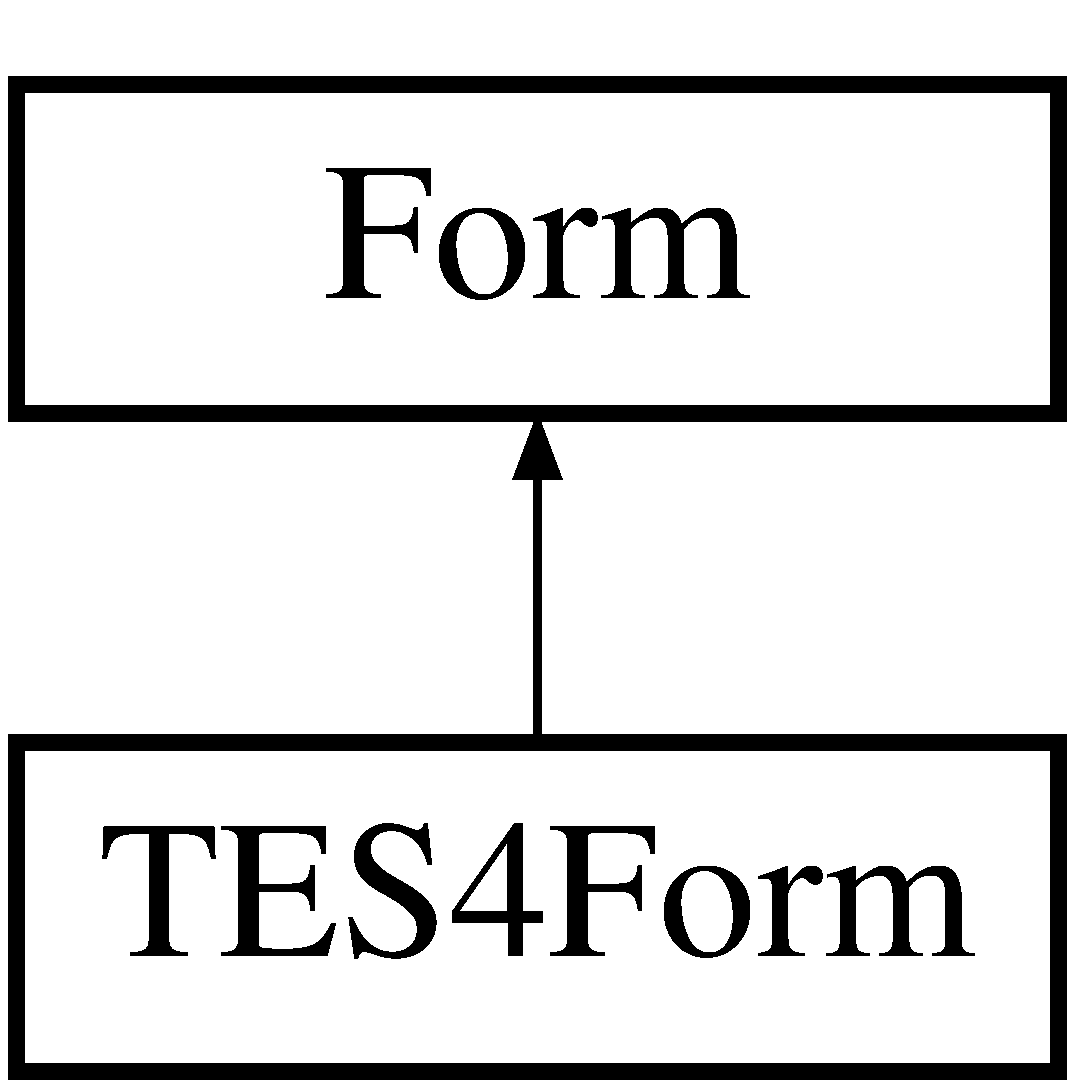
\includegraphics[height=2.000000cm]{class_t_e_s4_form}
\end{center}
\end{figure}
\subsection*{Public Member Functions}
\begin{DoxyCompactItemize}
\item 
\hyperlink{class_t_e_s4_form_a5d6ded3ee737f8bef51b9ae6bfc77c37}{T\+E\+S4\+Form} ()
\begin{DoxyCompactList}\small\item\em Initialise header with correct name. \end{DoxyCompactList}\item 
\hyperlink{class_t_e_s4_form_a634ebfa0b990061b23a158ab4192c140}{$\sim$\+T\+E\+S4\+Form} ()
\begin{DoxyCompactList}\small\item\em Destructs header object. \end{DoxyCompactList}\item 
void \hyperlink{class_t_e_s4_form_a1c485919edc03e15e2d346e1f61a8957}{load} (Q\+Data\+Stream $\ast$in)
\begin{DoxyCompactList}\small\item\em Loads the header. \end{DoxyCompactList}\end{DoxyCompactItemize}
\subsection*{Protected Attributes}
\begin{DoxyCompactItemize}
\item 
float \hyperlink{class_t_e_s4_form_ac43b3ea26b907f6a493377bd8bcaa433}{version}
\begin{DoxyCompactList}\small\item\em The version of the file parsed. \end{DoxyCompactList}\item 
int32\+\_\+t \hyperlink{class_t_e_s4_form_aa9442a2a6974797c0cbc80893eb1eb35}{records}
\begin{DoxyCompactList}\small\item\em The amount of records. \end{DoxyCompactList}\item 
uint32\+\_\+t \hyperlink{class_t_e_s4_form_ab88581c781ac52043756b241aaf81e0a}{next\+ID}
\begin{DoxyCompactList}\small\item\em The next object id. \end{DoxyCompactList}\item 
Q\+String \hyperlink{class_t_e_s4_form_adb8c90168e883d785ab821db06cef8cd}{author}
\begin{DoxyCompactList}\small\item\em The author of the file. \end{DoxyCompactList}\item 
Q\+String \hyperlink{class_t_e_s4_form_aa530f6d5b35d9ace03c4f8a0cd56d4ca}{desc}
\begin{DoxyCompactList}\small\item\em The description of the file. \end{DoxyCompactList}\item 
Q\+Map$<$ Q\+String, uint64\+\_\+t $>$ \hyperlink{class_t_e_s4_form_a4456691dfb90f6f6e7cd734fd6ac5ceb}{masters} \mbox{[}$\,$\mbox{]}
\begin{DoxyCompactList}\small\item\em The masterfiles of this file\textquotesingle{}s names and sizes. \end{DoxyCompactList}\item 
uint32\+\_\+t \hyperlink{class_t_e_s4_form_ab3ed4c6fda85359543c27f80bb118247}{intv}
\begin{DoxyCompactList}\small\item\em Unknown. \end{DoxyCompactList}\item 
uint32\+\_\+t \hyperlink{class_t_e_s4_form_a66402e4e8d8c7ada7380af8c4fd3518c}{incc}
\begin{DoxyCompactList}\small\item\em Unknown. \end{DoxyCompactList}\item 
Form\+Name \hyperlink{class_form_a3a19912be281bc3e9c99911bb70e0f4b}{name}
\begin{DoxyCompactList}\small\item\em Name of the form. \end{DoxyCompactList}\item 
\hyperlink{struct_form_header}{Form\+Header} \hyperlink{class_form_a6aec4c07386c72bb12947f7766562856}{header}
\begin{DoxyCompactList}\small\item\em The form\textquotesingle{}s header. \end{DoxyCompactList}\end{DoxyCompactItemize}


\subsection{Detailed Description}
The class for the T\+E\+S4 header. 

The class for the T\+E\+S4 header in .esp and .esm files. 

\subsection{Constructor \& Destructor Documentation}
\mbox{\Hypertarget{class_t_e_s4_form_a5d6ded3ee737f8bef51b9ae6bfc77c37}\label{class_t_e_s4_form_a5d6ded3ee737f8bef51b9ae6bfc77c37}} 
\index{T\+E\+S4\+Form@{T\+E\+S4\+Form}!T\+E\+S4\+Form@{T\+E\+S4\+Form}}
\index{T\+E\+S4\+Form@{T\+E\+S4\+Form}!T\+E\+S4\+Form@{T\+E\+S4\+Form}}
\subsubsection{\texorpdfstring{T\+E\+S4\+Form()}{TES4Form()}}
{\footnotesize\ttfamily T\+E\+S4\+Form\+::\+T\+E\+S4\+Form (\begin{DoxyParamCaption}{ }\end{DoxyParamCaption})}



Initialise header with correct name. 

Initialise header with the correct name enum (Header). \mbox{\Hypertarget{class_t_e_s4_form_a634ebfa0b990061b23a158ab4192c140}\label{class_t_e_s4_form_a634ebfa0b990061b23a158ab4192c140}} 
\index{T\+E\+S4\+Form@{T\+E\+S4\+Form}!````~T\+E\+S4\+Form@{$\sim$\+T\+E\+S4\+Form}}
\index{````~T\+E\+S4\+Form@{$\sim$\+T\+E\+S4\+Form}!T\+E\+S4\+Form@{T\+E\+S4\+Form}}
\subsubsection{\texorpdfstring{$\sim$\+T\+E\+S4\+Form()}{~TES4Form()}}
{\footnotesize\ttfamily T\+E\+S4\+Form\+::$\sim$\+T\+E\+S4\+Form (\begin{DoxyParamCaption}{ }\end{DoxyParamCaption})}



Destructs header object. 

Destructs header object in memory. 

\subsection{Member Function Documentation}
\mbox{\Hypertarget{class_t_e_s4_form_a1c485919edc03e15e2d346e1f61a8957}\label{class_t_e_s4_form_a1c485919edc03e15e2d346e1f61a8957}} 
\index{T\+E\+S4\+Form@{T\+E\+S4\+Form}!load@{load}}
\index{load@{load}!T\+E\+S4\+Form@{T\+E\+S4\+Form}}
\subsubsection{\texorpdfstring{load()}{load()}}
{\footnotesize\ttfamily void T\+E\+S4\+Form\+::load (\begin{DoxyParamCaption}\item[{Q\+Data\+Stream $\ast$}]{in }\end{DoxyParamCaption})\hspace{0.3cm}{\ttfamily [virtual]}}



Loads the header. 

Loads the T\+E\+S4 header from the data stream. 
\begin{DoxyParams}{Parameters}
{\em in} & The data stream to load the file from. \\
\hline
\end{DoxyParams}


Implements \hyperlink{class_form}{Form}.



\subsection{Member Data Documentation}
\mbox{\Hypertarget{class_t_e_s4_form_adb8c90168e883d785ab821db06cef8cd}\label{class_t_e_s4_form_adb8c90168e883d785ab821db06cef8cd}} 
\index{T\+E\+S4\+Form@{T\+E\+S4\+Form}!author@{author}}
\index{author@{author}!T\+E\+S4\+Form@{T\+E\+S4\+Form}}
\subsubsection{\texorpdfstring{author}{author}}
{\footnotesize\ttfamily Q\+String T\+E\+S4\+Form\+::author\hspace{0.3cm}{\ttfamily [protected]}}



The author of the file. 

The author of the file. Note\+: Optional \mbox{\Hypertarget{class_t_e_s4_form_aa530f6d5b35d9ace03c4f8a0cd56d4ca}\label{class_t_e_s4_form_aa530f6d5b35d9ace03c4f8a0cd56d4ca}} 
\index{T\+E\+S4\+Form@{T\+E\+S4\+Form}!desc@{desc}}
\index{desc@{desc}!T\+E\+S4\+Form@{T\+E\+S4\+Form}}
\subsubsection{\texorpdfstring{desc}{desc}}
{\footnotesize\ttfamily Q\+String T\+E\+S4\+Form\+::desc\hspace{0.3cm}{\ttfamily [protected]}}



The description of the file. 

The description of the file. Note\+: Optional \mbox{\Hypertarget{class_form_a6aec4c07386c72bb12947f7766562856}\label{class_form_a6aec4c07386c72bb12947f7766562856}} 
\index{T\+E\+S4\+Form@{T\+E\+S4\+Form}!header@{header}}
\index{header@{header}!T\+E\+S4\+Form@{T\+E\+S4\+Form}}
\subsubsection{\texorpdfstring{header}{header}}
{\footnotesize\ttfamily \hyperlink{struct_form_header}{Form\+Header} Form\+::header\hspace{0.3cm}{\ttfamily [protected]}, {\ttfamily [inherited]}}



The form\textquotesingle{}s header. 

The header of the form, with needed data for the parser. \mbox{\Hypertarget{class_t_e_s4_form_a66402e4e8d8c7ada7380af8c4fd3518c}\label{class_t_e_s4_form_a66402e4e8d8c7ada7380af8c4fd3518c}} 
\index{T\+E\+S4\+Form@{T\+E\+S4\+Form}!incc@{incc}}
\index{incc@{incc}!T\+E\+S4\+Form@{T\+E\+S4\+Form}}
\subsubsection{\texorpdfstring{incc}{incc}}
{\footnotesize\ttfamily uint32\+\_\+t T\+E\+S4\+Form\+::incc\hspace{0.3cm}{\ttfamily [protected]}}



Unknown. 

An unknown value. Note\+: Optional \mbox{\Hypertarget{class_t_e_s4_form_ab3ed4c6fda85359543c27f80bb118247}\label{class_t_e_s4_form_ab3ed4c6fda85359543c27f80bb118247}} 
\index{T\+E\+S4\+Form@{T\+E\+S4\+Form}!intv@{intv}}
\index{intv@{intv}!T\+E\+S4\+Form@{T\+E\+S4\+Form}}
\subsubsection{\texorpdfstring{intv}{intv}}
{\footnotesize\ttfamily uint32\+\_\+t T\+E\+S4\+Form\+::intv\hspace{0.3cm}{\ttfamily [protected]}}



Unknown. 

An unknown value, likely internal version. \mbox{\Hypertarget{class_t_e_s4_form_a4456691dfb90f6f6e7cd734fd6ac5ceb}\label{class_t_e_s4_form_a4456691dfb90f6f6e7cd734fd6ac5ceb}} 
\index{T\+E\+S4\+Form@{T\+E\+S4\+Form}!masters@{masters}}
\index{masters@{masters}!T\+E\+S4\+Form@{T\+E\+S4\+Form}}
\subsubsection{\texorpdfstring{masters}{masters}}
{\footnotesize\ttfamily Q\+Map$<$Q\+String, uint64\+\_\+t$>$ T\+E\+S4\+Form\+::masters\mbox{[}$\,$\mbox{]}\hspace{0.3cm}{\ttfamily [protected]}}



The masterfiles of this file\textquotesingle{}s names and sizes. 

The masterfiles of this file\textquotesingle{}s names and sizes. Note\+: In T\+E\+S4/\+T\+E\+S5, size is constant 0. \mbox{\Hypertarget{class_form_a3a19912be281bc3e9c99911bb70e0f4b}\label{class_form_a3a19912be281bc3e9c99911bb70e0f4b}} 
\index{T\+E\+S4\+Form@{T\+E\+S4\+Form}!name@{name}}
\index{name@{name}!T\+E\+S4\+Form@{T\+E\+S4\+Form}}
\subsubsection{\texorpdfstring{name}{name}}
{\footnotesize\ttfamily Form\+Name Form\+::name\hspace{0.3cm}{\ttfamily [protected]}, {\ttfamily [inherited]}}



Name of the form. 

The name of the form. \mbox{\Hypertarget{class_t_e_s4_form_ab88581c781ac52043756b241aaf81e0a}\label{class_t_e_s4_form_ab88581c781ac52043756b241aaf81e0a}} 
\index{T\+E\+S4\+Form@{T\+E\+S4\+Form}!next\+ID@{next\+ID}}
\index{next\+ID@{next\+ID}!T\+E\+S4\+Form@{T\+E\+S4\+Form}}
\subsubsection{\texorpdfstring{next\+ID}{nextID}}
{\footnotesize\ttfamily uint32\+\_\+t T\+E\+S4\+Form\+::next\+ID\hspace{0.3cm}{\ttfamily [protected]}}



The next object id. 

The next available object id. \mbox{\Hypertarget{class_t_e_s4_form_aa9442a2a6974797c0cbc80893eb1eb35}\label{class_t_e_s4_form_aa9442a2a6974797c0cbc80893eb1eb35}} 
\index{T\+E\+S4\+Form@{T\+E\+S4\+Form}!records@{records}}
\index{records@{records}!T\+E\+S4\+Form@{T\+E\+S4\+Form}}
\subsubsection{\texorpdfstring{records}{records}}
{\footnotesize\ttfamily int32\+\_\+t T\+E\+S4\+Form\+::records\hspace{0.3cm}{\ttfamily [protected]}}



The amount of records. 

The amount of records in the parsed file. \mbox{\Hypertarget{class_t_e_s4_form_ac43b3ea26b907f6a493377bd8bcaa433}\label{class_t_e_s4_form_ac43b3ea26b907f6a493377bd8bcaa433}} 
\index{T\+E\+S4\+Form@{T\+E\+S4\+Form}!version@{version}}
\index{version@{version}!T\+E\+S4\+Form@{T\+E\+S4\+Form}}
\subsubsection{\texorpdfstring{version}{version}}
{\footnotesize\ttfamily float T\+E\+S4\+Form\+::version\hspace{0.3cm}{\ttfamily [protected]}}



The version of the file parsed. 

The version of the .esm/.esp file parsed. 

The documentation for this class was generated from the following files\+:\begin{DoxyCompactItemize}
\item 
C\+:/\+Users/alexa/\+Documents/\+Coding/\+Qt/why/openck/\+Open\+C\+K/include/define/tes4form.\+h\item 
C\+:/\+Users/alexa/\+Documents/\+Coding/\+Qt/why/openck/\+Open\+C\+K/src/define/tes4form.\+cpp\end{DoxyCompactItemize}

%--- End generated contents ---

% Index
\backmatter
\newpage
\phantomsection
\clearemptydoublepage
\addcontentsline{toc}{chapter}{Index}
\printindex

\end{document}
